%%%%%%%%%%%%%%%%%%%%%%%%%%%%%%%%%%%%%%%%%%%%%%%%%%%%%%%%%%%%%%%%%%%%%%
% Lớp 11 | Hàm số mũ và hàm số lôgarít | Phương trình, bất phương trình mũ và lôgarít
% Dạng 1D6?4-4: Phương trình mũ, lôgarít đưa về cùng cơ số
% Số câu: 141  (sinh tự động bởi tach_cau.py; từ nay thầy sửa trực tiếp file này)
%%%%%%%%%%%%%%%%%%%%%%%%%%%%%%%%%%%%%%%%%%%%%%%%%%%%%%%%%%%%%%%%%%%%%%

%%%%%%%%%%%%%%%% TRẮC NGHIỆM 4 PHƯƠNG ÁN %%%%%%%%%%%%%%%%

% nguồn: Ok_Toan11_TracNghiem_Lan2
\begin{ex}%[1D6N4-4]%[ma:eb4aeb43]
	 Giải phương trình $(2{,}5)^{5x-7}=\left(\dfrac{2}{5}\right)^{x+1}$.
	\choice 
		{$x\geq  1$}
		{\True $x=1$} 
		 {$x<1$}
		 {$x=2$}
	 \loigiai{
		Ta có 
		\begin{eqnarray*}
			& &  (2{,}5)^{5x-7} = \left(\dfrac{2}{5}\right)^{x+1} \\
			&\Leftrightarrow  & \left(\dfrac{5}{2}\right)^{5x-7} = \left(\dfrac{5}{2}\right)^{-x-1} \\
			&\Leftrightarrow  & 5x-7 = -x-1 \\
			&\Leftrightarrow  & x=1.
		\end{eqnarray*}
	} 
\end{ex}

% nguồn: Ok_Toan11_TracNghiem_Lan2
\begin{ex}%[1D6N4-4]%[ma:f1320bff]
	Nghiệm của phương trình  $5^{x-1}=\dfrac{1}{25}$ là
	 \choice
		{$3$} 
		{$1$} 
		{\True  $-1$}
		{$-3$} 
	\loigiai{ 
		\begin{eqnarray*}
			& &  5^{x-1} = \dfrac{1}{25} \\
			&\Leftrightarrow & 5^{x-1}=5^{-2}  \\
			&\Leftrightarrow & x-1 = -2  \\
			 &\Leftrightarrow & x=-1.
		\end{eqnarray*}
	} 
\end{ex}

% nguồn: Ok_Toan11_TracNghiem_Lan2
\begin{ex}%[1D6N4-4]%[ma:56942661]
	Nghiệm của  phương trình $2^{3x}=64$ là
	 \choice
		{\True  $2$}
		 {$4$}
		{$3$} 
		 {$5$}
	\loigiai{ 
		Ta  có
		\begin{eqnarray*}
			&  & 2^{3x}=64 \\
			 &\Leftrightarrow & 2^{3x}=2^6 \\
			&\Leftrightarrow &  3x=6 \\
			&\Leftrightarrow  & x=2.
		\end{eqnarray*}
	} 
\end{ex}

% nguồn: Ok_Toan11_TracNghiem_Lan2
\begin{ex}%[1D6N4-4]%[ma:152897c2]
	Nghiệm của phương trình $3^{x-1}=27$ là 
	 \choice
		 {$x=5$}
		 {\True $x=4$}
		 {$x=3$}
		 {$x=2$}
	\loigiai{ 
		Ta có 
		\begin{eqnarray*}
			& &  3^{x-1}=27 \\
			&\Leftrightarrow & x-1=3 \\ 
			&\Leftrightarrow  & x=4.
		\end{eqnarray*}
		Vậy $x=4$ là nghiệm của phương trình. 
	 }
\end{ex}

% nguồn: Ok_Toan11_TracNghiem_Lan2
\begin{ex}%[1D6N4-4]%[ma:4497c1a4]
	Nghiệm của phương trình  $2^{3x-5}=16$ là
	 \choice
		 {\True $x=3$}
		{$x=2$} 
		{$x=7$} 
		{$x=\dfrac{1}{3}$} 
	 \loigiai{
		Ta  có
		\begin{eqnarray*}
			& & 2^{3x-5}=16  \\
			&\Leftrightarrow & 2^{3x-5}=2^4  \\
			 &\Leftrightarrow & 3x-5=4 \\
			&\Leftrightarrow  & x=3.
		\end{eqnarray*}
	 }
\end{ex}

% nguồn: Ok_Toan11_TracNghiem_Lan2
\begin{ex}%[1D6N4-4]%[ma:f2f2541d]
	$x=2$  là nghiệm của phương trình nào sau đây?
	\choice 
		 {$3^x=8$}
		{\True  $4^x=16$}
		 {$x^3=9$}
		{$16^x=4$} 
	 \loigiai{
		\begin{eqnarray*}
			& & 4^x=16  \\
			&\Leftrightarrow & 4^x=4^2 \\ 
			&\Leftrightarrow &  x=2.
		\end{eqnarray*}
	 }
\end{ex}

% nguồn: Ok_Toan11_TracNghiem_Lan2
\begin{ex}%[1D6N4-4]%[ma:6b3a7b6a]
	Nghiệm của phương trình  $(2{,}4)^{3x+1}=\left(\dfrac{5}{12}\right)^{x-9}$ là
	 \choice
		{$x=-2$} 
		{$x=-5$} 
		{$x=5$} 
		 {\True $x=2$}
	 \loigiai{
		 Ta có
		\begin{eqnarray*}
			&  & (2,4)^{3x+1} = \left(\dfrac{5}{12}\right)^{x-9} \\
			&\Leftrightarrow & \left(\dfrac{12}{5}\right)^{3x+1}  = \left(\dfrac{5}{12}\right)^{x-9} \\
			&\Leftrightarrow  & \left(\dfrac{5}{12}\right)^{-3x-1} = \left(\dfrac{5}{12}\right)^{x-9} \\
			&\Leftrightarrow &  -3x-1=x-9 \\
			&\Leftrightarrow & 4x=8 \\ 
			&\Leftrightarrow & x=2. 
		\end{eqnarray*}
		Vậy phương trình đã cho có nghiệm duy nhất một nghiệm  $x=2$.
	 }
\end{ex}

% nguồn: Ok_Toan11_TracNghiem_Lan2
\begin{ex}%[1D6N4-4]%[ma:0e89b75e]
	Phương trình  $\left(\sqrt{3}\right)^{3x-6}=1$ có nghiệm là:
	 \choice
		 {$x=0$}
		{\True $x=2$} 
		{$x=\dfrac{7}{3}$} 
		 {$x=6$}
	 \loigiai{
		 Phương trình
		\begin{eqnarray*}
			& &  \left(\sqrt{3}\right)^{3x-6}=1 \\
			 &\Leftrightarrow & 3x-6=0 \\
			&\Leftrightarrow  & x=2.
		\end{eqnarray*}
	 }
\end{ex}

% nguồn: Ok_Toan11_TracNghiem_Lan2
\begin{ex}%[1D6N4-4]%[ma:bb260c44]
	 Nghiệm của phương trình $3^x=1$ là
	 \choice
		 {\True $x=0$}
		{$x=1$} 
		 {$x=2$}
		{$x=-1$} 
	\loigiai{ 
		Ta có 
		\begin{eqnarray*}
			& & 3^x=1 \\ 
			&\Leftrightarrow  & 3^x=3^0 \\
			 &\Leftrightarrow & x=0.
		\end{eqnarray*}
	 }
\end{ex}

% nguồn: Ok_Toan11_TracNghiem_Lan2
\begin{ex}%[1D6N4-4]%[ma:22903c93]
	Nghiệm  của phương trình $4^{2x+1}=64$ là
	 \choice
		{$x=2$} 
		{$x=\dfrac{15}{2}$} 
		{$x=15$} 
		 {\True $x=1$}
	\loigiai{ 
		Ta có 
		\begin{eqnarray*}
			 & & 4^{2x+1}=64 \\
			&\Leftrightarrow  & 4^{2x+1}=4^3 \\
			&\Leftrightarrow  & 2x+1=3 \\
			 &\Leftrightarrow & x=1.
		\end{eqnarray*}
	 }
\end{ex}

% nguồn: Ok_Toan11_TracNghiem_Lan2
\begin{ex}%[1D6N4-4]%[ma:de8d26a4]
	Nghiệm của phương trình  $3^{x+1}=\left(\dfrac{1}{9}\right)^{2x}$ là:
	 \choice
		 {$x=1$}
		 {$x=-1$}
		 {$x=\dfrac{1}{5}$}
		 {\True $x=-\dfrac{1}{5}$}
	\loigiai{ 
		\begin{eqnarray*}
			& & 3^{x+1} = \left(\dfrac{1}{9}\right)^{2x}  \\
			&\Leftrightarrow & 3^{x+1} = 3^{-4x}  \\
			&\Leftrightarrow & x+1 = -4x  \Leftrightarrow x = -\dfrac{1}{5}.
		\end{eqnarray*}
	} 
\end{ex}

% nguồn: Ok_Toan11_TracNghiem_Lan2
\begin{ex}%[1D6N4-4]%[ma:4fff2bef]
	Nghiệm của phương trình  $2^{2x+3}=2^{x+7}$ là:
	\choice 
		 {$x=\dfrac{10}{3}$}
		{$x=\dfrac{4}{3}$} 
		 {\True $x=4$}
		 {$x=10$}
	 \loigiai{
		\begin{eqnarray*}
			& &  2^{2x+3}=2^{x+7} \\
			&\Leftrightarrow & 2x+3=x+7 \\ 
			&\Leftrightarrow  & x=4.
		\end{eqnarray*}
		Vậy phương trình có nghiệm  duy nhất $x=4$.
	 }
\end{ex}

% nguồn: Ok_TracNghiemLop11_Lan1
\begin{ex}%[1D6N4-4]%[ma:13939cf6]
	Tập nghiệm của phương trình $\log _{3}(2x-1)=\log _{3}(x-1)$  là
	\choice 
		{$S=\varnothing$} 
		{$S=\{-2\}$} 
		{$S=\{3\}$} 
		{\True $S=\{2\}$} 
	 \loigiai{
		Điều kiện: $x>1$.\\ 
		Phương trình tương đương $\Leftrightarrow  2x-1=x-1\Leftrightarrow x=2$.\\
		So với điều kiện ta được tập  nghiệm $S=\{2\}$.
	} 
\end{ex}

% nguồn: Ok_TracNghiemLop11_Lan1
\begin{ex}%[1D6N4-4]%[ma:5e2cd335]
	Phương trình $3^{x-2}=\dfrac{1}{9}$ có  nghiệm
	 \choice
		{\True $x=0$} 
		{$x=2$} 
		{$x=4$} 
		{$x=\dfrac{19}{9}$} 
	\loigiai{ 
		Ta có $3^{x-2}=\dfrac{1}{9} \Leftrightarrow 3^{x-2}=3^{-2} \Leftrightarrow x-2=-2  \Leftrightarrow x=0$.
	 }
\end{ex}

% nguồn: Ok_TracNghiemLop11_Lan1
\begin{ex}%[1D6N4-4]%[ma:b142d860]
	Phương trình $\log _{3}(2x+1)-\log _{3}(x-1)=1$  tương đương với hệ nào sau đây?
	 \choice
		 {$\heva{&x>-\dfrac{1}{2}\\&2x+1=x-1}$}
		 {$\heva{&x>-\dfrac{1}{2}\\&\dfrac{2x+1}{x-1}=1}$}
		{$\heva{&x>1\\&\dfrac{2x+1}{x-1}=1}$} 
		{\True  $\heva{&x>1\\&2x+1=3(x-1)}$}
	\loigiai{ 
		Điều kiện: $\heva{&2x+1>0\\&x-1>0}\Leftrightarrow  x>1$.\\
		Phương trình tương đương $\log _{3}(2x+1)=\log _{3}(x-1)+\log _{3}3\Leftrightarrow 2x+1=3(x-1)$. 
	 }
\end{ex}

% nguồn: Ok_TracNghiemLop11_Lan1
\begin{ex}%[1D6N4-4]%[ma:3fecc481]
	Nghiệm  của phương trình $\log_3(5x)=2$ là
	 \choice
		 {$x=\dfrac{8}{5}$}
		 {$x=9$}
		{\True  $x=\dfrac{9}{5}$}
		 {$x=8$}
	 \loigiai{
		Ta có $\log_3(5x)=2\Leftrightarrow 5x=9\Leftrightarrow x=\dfrac{9}{5}$. 
	} 
\end{ex}

% nguồn: Ok_TracNghiemLop11_Lan1
\begin{ex}%[1D6N4-4]%[ma:207835ab]
	Phương trình $5^{x+2}-1=0$ có tập  nghiệm là
	 \choice
		{$S=\{3\}$} 
		{$S=\{2\}$} 
		{$S=\{0\}$} 
		 {\True $S=\{-2\}$}
	\loigiai{ 
		Ta có  $5^{x+2}-1=0\Leftrightarrow 5^{x+2}=1\Leftrightarrow x+2=0\Leftrightarrow x=-2$.\\
		Vậy tập nghiệm của  phương trình là $S=\{-2\}$.
	 }
\end{ex}

% nguồn: Ok_TracNghiemLop11_Lan1
\begin{ex}%[1D6N4-4]%[ma:ba7a15e3]
	Nghiệm của phương trình $3^{x-1}=27$  là
	\choice 
		{$x=10$} 
		{\True $x=4$} 
		 {$x=9$}
		 {$x=3$}
	 \loigiai{
		Ta có  $3^{x-1}=27\Leftrightarrow 3^{x-1}=3^{3}\Leftrightarrow x-1=3\Leftrightarrow x=4$.\\
		Vậy phương trình có nghiệm $x=4$. 
	} 
\end{ex}

% nguồn: Ok_TracNghiemLop11_Lan1
\begin{ex}%[1D6N4-4]%[ma:f1a7252e]
	Nếu $\log  x=2\log7-\log5$ thì
	\choice 
		{$x=\dfrac{14}{5}$} 
		 {$44$}
		{\True $x=\dfrac{49}{5}$} 
		{$2$} 
	 \loigiai{
		 Điều kiện $x>0$.\\
		Ta có $\log x=2\log7-\log5\Leftrightarrow \log x=\log  7^2-\log 5\Leftrightarrow\log x=\log\dfrac{49}{5}$.\\
		Vậy  $x=\dfrac{49}{5}$.
	 }
\end{ex}

% nguồn: Ok_Toan11_TracNghiem_Lan2
\begin{ex}%[1D6H4-4]%[ma:15c76070]
	Tập nghiệm của bất phương trình $2^{x^2-2x-3}=1$  là
	 \choice
		 {$S=\{1;-3\}$}
		 {$S=\{2\}$}
		{\True  $S=\{-1;3\}$}
		{$S=\{0\}$} 
	\loigiai{ 
		Ta có 
		\begin{eqnarray*}
			&  & 2^{x^2-2x-3} = 1 \\
			&\Leftrightarrow & x^2-2x-3 =  0 \\
			&\Leftrightarrow & \left[\begin{array}{l} x=-1 \\ x=3.
		\end{array}\right.
	\end{eqnarray*}
	Tập nghiệm của bất phương trình  $2^{x^2-2x-3}=1$ là $S=\{-1;3\}$.
} 
\end{ex}

% nguồn: Ok_Toan11_TracNghiem_Lan2
\begin{ex}%[1D6H4-4]%[ma:4aefe070]
	Tổng tất cả các nghiệm  của phương trình $2^{x^2+2x}=8^{2-x}$ bằng
	 \choice
		 {\True $-5$}
		{$-6$} 
		{$5$} 
		{$6$} 
	 \loigiai{
		 Ta có
		\begin{eqnarray*}
			& & 2^{x^2+2x} = 8^{2-x}  \\
			&\Leftrightarrow &  2^{x^2+2x} = 2^{6-3x} \\
			&\Leftrightarrow  & x^2+2x=6-3x \\
			&\Leftrightarrow &  x^2+5x-6=0 \\
			&\Leftrightarrow & \left[\begin{array}{l} x=1 \\ x=-6.
		\end{array}\right.
	\end{eqnarray*}
	Tổng tất cả các nghiệm của  phương trình là $1+(-6)=-5$.
 }
\end{ex}

% nguồn: Ok_Toan11_TracNghiem_Lan2
\begin{ex}%[1D6H4-4]%[ma:9abda40e]
	Tổng bình phương các nghiệm của phương trình $3^{x^2-4x+5}=9$ là 
	 \choice
		 {$12$}
		{\True  $10$}
		{$11$} 
		{$9$} 
	\loigiai{ 
		\begin{eqnarray*}
			&  & 3^{x^2-4x+5} = 9 \\
			&\Leftrightarrow  & x^2-4x+5 = \log_3 9 \\
			&\Leftrightarrow & x^2-4x+3=0 \\ 
			&\Leftrightarrow & \left[\begin{array}{l} x_1=1 \\ x_2=3
		\end{array}\right. \Rightarrow x_1^2+x_2^2=10.
	\end{eqnarray*}
} 
\end{ex}

% nguồn: Ok_Toan11_TracNghiem_Lan2
\begin{ex}%[1D6H4-4]%[ma:72454aea]
	Tổng các  nghiệm của phương trình $2^{x^2}=4^{2x}$ là:
	\choice 
		{$0$} 
		{\True $4$} 
		{$1$} 
		 {$2$}
	\loigiai{ 
		Ta có 
		\begin{eqnarray*}
			& & 2^{x^2} = 4^{2x} \\ 
			&\Leftrightarrow & 2^{x^2}  = 2^{4x} \\
			&\Leftrightarrow & x^2-4x=0 \\ 
			&\Leftrightarrow & \left[\begin{array}{l} x=0 \\ x=4.
		\end{array}\right.
	\end{eqnarray*}
	Vậy tổng các nghiệm của  phương trình là $4+0=4$.
} 
\end{ex}

% nguồn: Ok_Toan11_TracNghiem_Lan2
\begin{ex}%[1D6H4-4]%[ma:3e0f3cf3]
	Tập nghiệm của phương trình: $3^{x^2-3x+2}=1$  là:
	 \choice
		{$I=3$} 
		{\True  $S=\{1;2\}$}
		{$S=\{1\}$} 
		 {$S=\{2\}$}
	\loigiai{ 
		Ta có 
		\begin{eqnarray*}
			& &  3^{x^2-3x+2} = 1 \\
			&\Leftrightarrow &  x^2-3x+2=0 \\
			&\Leftrightarrow & \left[\begin{array}{l} x=1 \\ x=2.
		\end{array}\right.
	\end{eqnarray*}
	Vậy tập nghiệm  của phương trình là $S=\{1;2\}$.
 }
\end{ex}

% nguồn: Ok_Toan11_TracNghiem_Lan2
\begin{ex}%[1D6H4-4]%[ma:b5b3cd68]
	Cho phương trình $2^{x^2-x+8} - 4^{1-3x}=0$  có hai nghiệm $x_1; x_2$. Tính $S=x_1+x_2$.
	 \choice
		 {$S=2$}
		{$S=-1$} 
		 {$S=4$}
		{\True $S=-5$} 
	 \loigiai{
		Phương trình 
		\begin{eqnarray*}
			& & 2^{x^2-x+8} - 4^{1-3x} = 0 \\ 
			&\Leftrightarrow & 2^{x^2-x+8}  = 4^{1-3x} \\
			&\Leftrightarrow & 2^{x^2-x+8} =  2^{2(1-3x)} \\
			&\Leftrightarrow & x^2-x+8  = 2-6x \\
			&\Leftrightarrow &  x^2+5x+6=0.
		\end{eqnarray*}
		Vậy $S  = x_1 + x_2 = -5$.
	 }
\end{ex}

% nguồn: Ok_Toan11_TracNghiem_Lan2
\begin{ex}%[1D6H4-4]%[ma:ded6dcec]
	Phương trình $5^{x^2-1}=25^{x+1}$ có tập  nghiệm là
	\choice 
		{\True $\{-1;3\}$} 
		{$\{1;3\}$} 
		 {$\{-3;1\}$}
		 {$\{-3;-1\}$}
	\loigiai{ 
		Ta có 
		\begin{eqnarray*}
			& & 5^{x^2-1} = 25^{x+1} \\ 
			&\Leftrightarrow &  5^{x^2-1} = 5^{2x+2} \\
			&\Leftrightarrow  & x^2-1=2x+2 \\
			&\Leftrightarrow & \left[\begin{array}{l} x=3 \\ x=-1.
		\end{array}\right.
	\end{eqnarray*}
	Vậy tập nghiệm  của phương trình $S=\{3;-1\}$.
 }
\end{ex}

% nguồn: Ok_Toan11_TracNghiem_Lan2
\begin{ex}%[1D6H4-4]%[ma:bb50e15d]
	Gọi $x_1$, $x_2$ là hai nghiệm của phương trình $7^{x+1}=\left(\dfrac{1}{7}\right)^{x^2-2x-3}$. Khi đó  $x_1+x_2$ bằng:
	 \choice
		 {$-2$}
		{$-1$} 
		 {$2$}
		{\True $1$} 
	\loigiai{ 
		\begin{eqnarray*}
			& & 7^{x+1} =  \left(\dfrac{1}{7}\right)^{x^2-2x-3} \\
			&\Leftrightarrow & 7^{x+1} = 7^{-(x^2-2x-3)}  \\
			&\Leftrightarrow  & x+1 = -x^2+2x+3 \\
			&\Leftrightarrow & x^2-x-2=0 \\ 
			&\Leftrightarrow & \left[\begin{array}{l} x_1=-1 \\ x_2=2.
		\end{array}\right.
	\end{eqnarray*}
	Vậy  $x_1+x_2=1$.
 }
\end{ex}

% nguồn: Ok_Toan11_TracNghiem_Lan2
\begin{ex}%[1D6H4-4]%[ma:7d26cfc9]
	 Phương trình $3^{x^2-3x}=81$ có tổng các nghiệm là
	 \choice
		{$-3$} 
		{\True  $3$}
		 {$-4$}
		{$-5$} 
	 \loigiai{
		Ta  có
		\begin{eqnarray*}
			& & 3^{x^2-3x} = 81 \\ 
			&\Leftrightarrow  & x^2-3x=4 \\
			&\Leftrightarrow & \left[\begin{array}{l} x=-1 \\ x=4.
		\end{array}\right.
	\end{eqnarray*}
	Vậy tổng  các nghiệm của phương trình là $3$.
 }
\end{ex}

% nguồn: Ok_Toan11_TracNghiem_Lan2
\begin{ex}%[1D6H4-4]%[ma:145c44ef]
	Số nghiệm dương của phương trình $\left(\dfrac{1}{3}\right)^{x^2-4x}=9$  là
	 \choice
		{\True  $2$}
		 {$1$}
		{$3$} 
		{$0$} 
	 \loigiai{
		Ta  có
		\begin{eqnarray*}
			 & & \left(\dfrac{1}{3}\right)^{x^2-4x}=9 \\
			&\Leftrightarrow  & x^2-4x=-2 \\
			&\Leftrightarrow & x^2-4x+2=0  \\
			&\Leftrightarrow &  x=2\pm\sqrt{2}.
		\end{eqnarray*}
		 Cả hai nghiệm của phương trình đều dương.
	 }
\end{ex}

% nguồn: Ok_Toan11_TracNghiem_Lan2
\begin{ex}%[1D6H4-4]%[ma:62c110a0]
	Số nghiệm  thực của phương trình $2^{\sqrt{x}}=2^{2-x}$ là:
	 \choice
		{\True $1$} 
		{$3$} 
		{$2$} 
		 {$0$}
	 \loigiai{
		Ta có 
		\begin{eqnarray*}
			&  & 2^{\sqrt{x}} = 2^{2-x} \\
			&\Leftrightarrow & \heva{&x \ge 0  \\ &\sqrt{x} = 2-x} \\
			 &\Leftrightarrow & x=1.
		\end{eqnarray*}
	 }
\end{ex}

% nguồn: Ok_Toan11_TracNghiem_Lan2
\begin{ex}%[1D6H4-4]%[ma:b655d071]
	 Số nghiệm của phương trình $3^{x^2-2x}=1$ là
	 \choice
		{$0$} 
		{\True $2$} 
		 {$3$}
		 {$4$}
	 \loigiai{
		Ta có 
		\begin{eqnarray*}
			& & 3^{x^2-2x} =  1 \\
			&\Leftrightarrow & 3^{x^2-2x} = 3^0 \\ 
			&\Leftrightarrow &  x^2-2x=0 \\
			&\Leftrightarrow & \left[\begin{array}{l} x=0 \\ x=2.
		\end{array}\right.
	\end{eqnarray*}
 }
\end{ex}

% nguồn: Ok_TracNghiemLop11_Lan1
\begin{ex}%[1D6H4-4]%[ma:caa787bc]
	Tập nghiệm $S$ của  phương trình $\log _{2}(x-1)=2\log _{4}(2x+1)$ là
	 \choice
		{\True $S=\varnothing$} 
		 {$S=\{2\}$}
		 {$S=\{-2\}$}
		 {$S=\{0\}$}
	 \loigiai{
		Ta  có
		\begin{eqnarray*}
			&&\log  _{2}(x-1)=2\log _{4}(2x+1)\\
			&\Leftrightarrow& \log _{2}(x-1)=\log _{2}(2x+1)\\ 
			 &\Leftrightarrow&\heva{&x-1>0\\&x-1=2x+1}\\
			 &\Leftrightarrow&\heva{&x>1\\&x=-2}\Leftrightarrow x\in \varnothing.
		\end{eqnarray*}
		Vậy  tập nghiệm của phương trình đã cho là $S=\varnothing$.
	 }
\end{ex}

% nguồn: Ok_TracNghiemLop11_Lan1
\begin{ex}%[1D6H4-4]%[ma:db2c78c6]
	Nghiệm của phương trình  $\log_3 \left(2x-1\right)=2$ là
	 \choice
		{$x=3$} 
		 {\True $x=5$}
		 {$x=\dfrac{9}{2}$}
		{$x=\dfrac{7}{2}$} 
	\loigiai{Điều kiện  $x>\dfrac{1}{2}$.\\
		 Khi đó bất phương trình tương đương
		$\log_3  \left(2x-1\right)=2\Leftrightarrow 2x-1=3^2\Leftrightarrow x=5$.\\
		Vậy $-x=5$. 
	 }
\end{ex}

% nguồn: Ok_TracNghiemLop11_Lan1
\begin{ex}%[1D6H4-4]%[ma:e8548520]
	Tổng bình phương các nghiệm của phương trình $5^{3x-2}=\left(\dfrac{1}{5}\right)^{-x^{2}}$ bằng 
	 \choice
		 {$0$}
		{\True $5$} 
		 {$2$}
		{$3$} 
	 \loigiai{
		Ta  có $5^{3x-2}=\left(\dfrac{1}{5}\right)^{-x^{2}}\Leftrightarrow 5^{3x-2}=5^{x^{2}}\Leftrightarrow 3x-2=x^{2}\Leftrightarrow\hoac{
		&x=1\\&x=2.}$\\ 
		Vậy  tổng bình phương hai nghiệm bằng $1^2 + 2^2 = 5$.
	 }
\end{ex}

% nguồn: Ok_TracNghiemLop11_Lan1
\begin{ex}%[1D6H4-4]%[ma:459f3802]
	Tổng các nghiệm của phương trình $2^{x^{2}-2x+1}=8$ bằng 
	 \choice
		 {$0$}
		{$-2$} 
		{\True $2$} 
		 {$1$}
	\loigiai{ 
		 Ta có $2^{x^{2}-2x+1}=8\Leftrightarrow 2^{x^{2}-2x+1}=2^{3}\Leftrightarrow x^{2}-2x+1=3\Leftrightarrow x^{2}-2x-2=0\Leftrightarrow\hoac{&x=1-\sqrt{3}\\&x=1+\sqrt{3}.}$\\
		Như  vậy phương trình đã cho có hai nghiệm $1-\sqrt{3}$ và $1+\sqrt{3}$.\\
		Vậy  tổng hai nghiệm là $\left(1-\sqrt{3}\right)+\left(1+\sqrt{3}\right)=2$.
	 }
\end{ex}

% nguồn: Ok_TracNghiemLop11_Lan1
\begin{ex}%[1D6H4-4]%[ma:50a92788]
	Phương  trình $2^{x}\cdot 5^{x^{2}-2x}=1$ có bao nhiêu nghiệm?
	\choice 
		{$1$} 
		{\True  $2$}
		 {$3$}
		{$0$} 
	 \loigiai{
		Ta có $2^{x}\cdot 5^{x^{2}-2x}=1\Leftrightarrow x\cdot \log _{5}2+x^{2}-2x=0\Leftrightarrow x\cdot \left(\log _{5}2+x-2\right)=0\Leftrightarrow\hoac{&x=0\\&x=2-\log _{5}2.}$\\ 
		Vậy phương trình  có hai nghiệm phân biệt.
	 }
\end{ex}

% nguồn: Ok_TracNghiemLop11_Lan1
\begin{ex}%[1D6H4-4]%[ma:8e3f80d7]
	Phương trình $\log _{5}(x+1)+\log _{\frac{1}{5}}(7-x)=0$ có  tập nghiệm là
	\choice 
		{$S=\{1\}$} 
		{$S=\{0\}$} 
		{\True  $S=\{3\}$}
		{$S=\{-\sqrt{7};\sqrt{7}\}$} 
	\loigiai{ 
		 Điều kiện: $\heva{&x+1>0\\&7-x>0}\Leftrightarrow-1<x<7$.\\
		Phương trình tương đương $\log _{5}(x+1)=\log _{5}(7-x)\Leftrightarrow x+1=7-x\Leftrightarrow  x=3$.\\
		 So với điều kiện ta được tập nghiệm $S=\{3\}$.
	} 
\end{ex}

% nguồn: Ok_TracNghiemLop11_Lan1
\begin{ex}%[1D6H4-4]%[ma:b567056b]
	Tìm số nghiệm của phương  trình $\log _2 x+\log _2(x-1)=2$.
	 \choice
		{$ 0$} 
		 {\True $1 $}
		 {$3 $}
		 {$2 $}
	 \loigiai{
		Điều kiện  $ \heva{&x>0\\&x-1>0}\Leftrightarrow x>1 $.\\
		 Ta có \allowdisplaybreaks
		\begin{eqnarray*}
			 && \log _2 x+\log _2(x-1)=2 \Leftrightarrow \log _2 [x(x-1)]=2\\
			&\Leftrightarrow& x(x-1)=2^2 \Leftrightarrow  x^2-x-4=0 \\
			&\Leftrightarrow&  \hoac{&x=\dfrac{1-\sqrt{17}}{2}&\text{(loại)}&\\&x=\dfrac{1+\sqrt{17}}{2}&\text{(nhận)}&.}
		\end{eqnarray*}
		Vậy phương trình đã cho có một nghiệm duy nhất $ x=\dfrac{1+\sqrt{17}}{2}  $.
	 }
\end{ex}

% nguồn: Ok_TracNghiemLop11_Lan1
\begin{ex}%[1D6H4-4]%[ma:37b69520]
	 Số nghiệm của phương trình $\log _{3}\left(3^{x}+2\right)=x+1$ là
	\choice 
		{\True $1$} 
		{$2$} 
		{$0$} 
		{$3$} 
	\loigiai{ 
		Ta có  $\log _{3}\left(3^{x}+2\right)=x+1\Leftrightarrow 3^{x}+2=3^{x+1}\Leftrightarrow 3^{x}+2=3\cdot 3^{x}\Leftrightarrow 3^{x}=1\Leftrightarrow x=0$.\\
		Vậy phương trình có duy nhất một  nghiệm $x=0$.
	} 
\end{ex}

% nguồn: Ok_TracNghiemLop11_Lan1
\begin{ex}%[1D6H4-4]%[ma:6e920cbf]
	Tích các nghiệm  của phương trình $\left(\sqrt{5}+2\right)^{x-1}=\left(\sqrt{5}-2\right)^{\tfrac{x-1}{x+1}}$ là
	\choice 
		{\True $-2$} 
		 {$-4$}
		 {$2$}
		{$4$} 
	\loigiai{ 
		 Điều kiện: $x\neq-1$.\\
		Vì  $\left(\sqrt{5}-2\right)\left(\sqrt{5}+2\right)=1$ nên $\left(\sqrt{5}-2\right)=\left(\sqrt{5}+2\right)^{-1}$.\\
		 Khi đó phương trình đã cho tương đương\\
		$\left(\sqrt{5}+2\right)^{x-1}=\left(\sqrt{5}+2\right)^{\tfrac{-x+1}{x+1}}\Leftrightarrow  x-1=\dfrac{-x+1}{x+1}\Leftrightarrow\hoac{&x=1\\&x=-2}$
		(thỏa  điều kiện).\\
		Suy ra tích hai nghiệm  là $1\cdot(-2)=-2$.
	} 
\end{ex}

% nguồn: Ok_TracNghiemLop11_Lan1
\begin{ex}%[1D6H4-4]%[ma:7e866c40]
	Phương trình $9^x-3\cdot 3^x+2=0$ có 2 nghiệm $x_1$,  $x_2$ với $x_1 < x_2$. Giá trị $2x_1+3x_2$ bằng
	\choice 
		{$4\log_2  3$}
		{$2$} 
		{$0$} 
		 {\True $3\log_3 2$}
	\loigiai{$9^x-3\cdot  3^x+2=0\Leftrightarrow \hoac{&3^x=1\\&3^x=2}\Leftrightarrow \hoac{&x=0\\&x=\log_32.}$\\
	 Khi đó $2x_1+3x_2=3\log_3 2.$ }
\end{ex}

% nguồn: Ok_TracNghiemLop11_Lan1
\begin{ex}%[1D6H4-4]%[ma:b968463c]
	Phương trình $\log (4x+1)=\log (2x+5)$  có nghiệm là
	\choice 
		{\True  $x=2$}
		 {$x=1$}
		 {$x=3$}
		{$x=-1$} 
	 \loigiai{Ta có $\log (4x+1)=\log (2x+5)\Leftrightarrow\heva{&4x+1>0\\&4x+1=2x+5}\Leftrightarrow \heva{&x>-\dfrac{1}{4}\\&x=2}\Leftrightarrow x=2$.}
\end{ex}

% nguồn: Ok_TracNghiemLop11_Lan1
\begin{ex}%[1D6H4-4]%[ma:232d4ad3]
	Nghiệm của  phương trình $2^{x-1}=3$ có dạng $a+\log _{b}3\,(a\in \mathbb{R},0<b\neq 1)$. Tính $S=a+b$.
	\choice 
		 {\True $3$}
		 {$2$}
		{$1$} 
		{$4$} 
	\loigiai{ 
		 Ta có $2^{x-1}=3\Leftrightarrow x-1=\log_{2}3\Leftrightarrow x=1+\log_{2}3$.\\
		 Suy ra $a=1$, $b=2$.\\
		Vậy  $S=a+b=3$.
	 }
\end{ex}

% nguồn: Ok_TracNghiemLop11_Lan1
\begin{ex}%[1D6H4-4]%[ma:4cdc3ec3]
	Tập nghiệm $S$ của phương trình $3^{x^2-2x}=27$. 
	 \choice
		{$S=\left\{1; 3\right\}$} 
		{$S=\left\{-3; 1\right\}$} 
		{\True $S=\left\{-1;  3\right\}$}
		 {$S=\left\{-3;-1\right\}$}
	\loigiai{ 
		$3^{x^2-2x}=27\Leftrightarrow x^2-2x=3\Leftrightarrow \hoac{&x=-1\\&x=3.}$\\ 
	Vậy tập  nghiệm phương trình $S=\left\{-1; 3\right\}$. }
\end{ex}

% nguồn: Ok_TracNghiemLop11_Lan1
\begin{ex}%[1D6H4-4]%[ma:b81911b0]
	Số nghiệm thực của  phương trình $3\log_3(x-1)-\log_{\tfrac{1}{3}}(x-5)^3=3$ là
	\choice 
		 {$3$}
		 {$2$}
		{\True  $1$}
		 {$0$}
	 \loigiai{
		Điều kiện:  $x>5$.\\
		Ta có \allowdisplaybreaks\begin{eqnarray*}
		 &&3\log_3(x-1)-\log_{\tfrac{1}{3}}(x-5)^3=3\\
		&\Leftrightarrow&  3\log_3(x-1)+3\log_3(x-5)=3 \\
		 &\Leftrightarrow&\log_3(x-1)+\log_3(x-5)=1\\
		&\Leftrightarrow&\log_3[(x-1)(x-5)]=1\\ 
		 &\Leftrightarrow&(x-1)(x-5)=3 \\
		& \Leftrightarrow& x^2-6x+2=0\Leftrightarrow  x=3\pm\sqrt{7}.
	\end{eqnarray*}
Đối chiếu điều kiện suy ra phương trình có $1$ nghiệm  $x=3+\sqrt{7}$.}
\end{ex}

% nguồn: Ok_TracNghiemLop11_Lan1
\begin{ex}%[1D6H4-4]%[ma:dec377e2]
	Tập nghiệm của bất phương  trình $2^{2+x^2}>16$ là
	\choice 
		{$(-\infty;-2)\cup  (2;+\infty)$}
		{\True $\left(-\infty;-\sqrt  {2} \right)\cup \left(\sqrt {2};+\infty \right)$}
		 {$(-\infty;-2)\cup [2;+\infty)$}
		{$\left(-\infty;-\sqrt {2} \right]\cup \left[\sqrt  {2};+\infty \right)$}
	 \loigiai{
	Ta có $2^{2+x^2}>16\Leftrightarrow 2+x^2>4\Leftrightarrow x^2>2\Leftrightarrow x\in \left(-\infty;-\sqrt {2}  \right)\cup \left(\sqrt {2};+\infty \right)$.
	} 
\end{ex}

% nguồn: Ok_TracNghiemLop11_Lan1
\begin{ex}%[1D6H4-4]%[ma:be53b5af]
	Tổng các nghiệm của phương trình $\log  _{\sqrt{3}} \left(x-2\right)+\log_3 \left(x-4\right)^2=0$ là $S=a+b\sqrt{2}$ (với $a, b$ là các số nguyên). Giá trị của biểu thức $Q=a+3b$ bằng
	 \choice
		 {$7$}
		{\True  $9$}
		{$6$} 
		{$8$} 
	\loigiai{Điều kiện  xác định $\heva{&x>2\\&x\not=4.}$\\
		Phương trình đã  cho tương đương với
		\begin{eqnarray*}
			& &  \log_3(x-2)^2+\log_3(x-4)^2=0\\
			 &\Leftrightarrow & \log_3(x-2)^2(x-4)^2=0\\
			&\Leftrightarrow &  (x-2)^2(x-4)^2=1\Leftrightarrow (x-2)|x-4|=1\Leftrightarrow\hoac{&(x-2)(x-4)=1\\&(x-2)(x-4)=-1.}
		\end{eqnarray*}
		Khi đó ta suy ra nghiệm phương trình là $\hoac{&x=3-\sqrt{2} \,(\text{loại})\\&x=3+\sqrt{2}\\&x=3.}$\\ 
		Vậy tổng các nghiệm của phương trình là  $S=3+3+\sqrt{2}=6+\sqrt{2}$ suy ra $a=6$, $b=1$.\\
		 Do đó giá trị của biểu thức $Q=a+3b=9$.
	} 
\end{ex}

% nguồn: Ok_TracNghiemLop11_Lan1
\begin{ex}%[1D6H4-4]%[ma:8ca9744c]
	 Tổng tất cả các nghiệm của phương trình $\log_2(x-1)+\log_2x =1+\log_2(3x-5)$ bằng
	\choice 
		{\True  $7$}
		 {$6$}
		 {$5$}
		{$4 $} 
	\loigiai{ 
		Điều kiện xác định $ x>\dfrac{5}{3}.  $\\
		Phương trình đã cho tương đương  với
		\begin{align*}
			&  \log_2(x(x-1))=\log_2(2(3x-5))\\
			\Leftrightarrow &  x^2-x =6x-10\\
			\Leftrightarrow & \hoac{&x=5\text{ (thỏa mãn)} \\&x=2.\text{  (thỏa mãn)}}
		\end{align*}
		Do đó tổng các nghiệm  của phương trình là $ 7 $.
	} 
\end{ex}

% nguồn: Ok_TracNghiemLop11_Lan1
\begin{ex}%[1D6H4-4]%[ma:1662dce5]
	Tập nghiệm của phương trình $\log _{2}\left(x^{2}-1\right)=3$  là
	 \choice
		 {$\{-3\}$}
		 {$\{3\}$}
		 {\True $\{-3;3\}$}
		{$\left\{-\sqrt{10};\sqrt{10}\right\}$} 
	 \loigiai{
		Điều kiện: $x^{2}-1>0\Leftrightarrow\hoac{&x<-1\\&x>1.}$\\ 
		Phương trình  tương đương với $x^{2}-1=2^{3}\Leftrightarrow\hoac{&x=-3\\&x=3.}$\\
		So với điều kiện  ta được tập nghiệm của phương trình là $S=\{-3;3\}$.
	} 
\end{ex}

% nguồn: Ok_TracNghiemLop11_Lan1
\begin{ex}%[1D6H4-4]%[ma:c244f9a2]
	Số nghiệm của phương trình $\log_3 \left(6+x\right)+\log_3 9x-5=0$  là
	\choice 
		{$2$} 
		 {\True $1$}
		{$0$} 
		{$3$} 
	\loigiai{Điều kiện xác  định của phương trình $x>0$.
		\begin{eqnarray*}
			& & \log_3  \left(6+x\right)+\log_3 9x-5=0\\
			 &\Leftrightarrow & \log_3\left(9x(6+x) \right)=5\\
			&\Leftrightarrow &  x(6+x)=27\Leftrightarrow x^2+6x-27=0\Leftrightarrow\hoac{&x=-9\\&x=3.}
		\end{eqnarray*}
	Vậy so với điều kiện ta chọn nghiệm $x=3$.} 
\end{ex}

% nguồn: Ok_TracNghiemLop11_Lan1
\begin{ex}%[1D6H4-4]%[ma:8241ec0a]
	Tìm tất cả các giá trị của tham số $m$ để phương trình $2^{2x+1}-2^{x+3}-2m=0$  có hai nghiệm phân biệt.
	 \choice
		{$m >  0$}
		{$m  >-4$}
		{\True $-4< m < 0$} 
		{$m  <-4$}
	 \loigiai{
		Đặt $t=2^x, \left(t  > 0\right)$.\\
		Phương trình  trở thành $2t^2-8t-2m=0$ (*)\\
		Phương trình  có 2 nghiệm phân biệt khi phương trình (*) có $2$ nghiệm dương phân biệt $$\Leftrightarrow \heva{&{\Delta ' > 0} \\
		 &{S> 0} \\
		 &{P> 0}} \Leftrightarrow \heva{&{16+4m > 0} \\
		&{m <  0}
		 &} \Leftrightarrow-4< m < 0.$$
	} 
\end{ex}

% nguồn: Ok_TracNghiemLop11_Lan1
\begin{ex}%[1D6V4-4]%[ma:2ef4fd62]
	Tính tích các  nghiệm của phương trình $\left(3+2\sqrt{2} \right)^{x^2-x+2}=\left(3-2\sqrt{2} \right)^{x^3-2}$
	 \choice
		{\True  $t=0$}
		{$t=2$} 
		 {$t=-1$}
		 {$t=1$}
	\loigiai{ 
		\begin{eqnarray*}
			& & \left(3+2\sqrt{2} \right)^{x^2-x+2}=\left(3-2\sqrt{2}  \right)^{x^3-2}\\
			&\Leftrightarrow & \left(3+2\sqrt{2} \right)^{x^2-x+2}=\dfrac{1}{\left(3+2\sqrt{2} \right)^{x^3-2}}\\ 
			&\Leftrightarrow & \left(3+2\sqrt{2} \right)^{x^2-x+2} \left(3+2\sqrt{2}  \right)^{x^3-2}=1\\
			 &\Leftrightarrow &\left(3+2\sqrt{2} \right)^{x^2-x+2+x^3-2}=1\\
			&\Leftrightarrow & x^3+x^2-x=0\Leftrightarrow \hoac{&x=0 \\&x=\dfrac{-1\pm \sqrt{5}}{2}}  \Rightarrow t=0.
		\end{eqnarray*}
	 }
\end{ex}

% nguồn: Ok_TracNghiemLop11_Lan1
\begin{ex}%[1D6V4-4]%[ma:c0f9f0ff]
	Gọi $x_1$, $x_2$ là nghiệm  của phương trình $\left(\sqrt{5}-2\right)^{2x^2+2^{100}x+6}=\left(9-4\sqrt{5}\right)^{x+3}$. Khi đó $x_1+x_2$ bằng
	\choice 
		 {$2^{100}-1$}
		{\True  $1-2^{99}$}
		 {$1-2^{100}$}
		{$2^{99}-1$} 
	\loigiai{ 
		Ta có 
		 \allowdisplaybreaks
		\begin{eqnarray*}
			\left(\sqrt{5}-2\right)^{2x^2+2^{100}x+6}=\left(9-4\sqrt{5}\right)^{x+3}&\Leftrightarrow&\left(\sqrt{5}-2\right)^{2x^2+2^{100}x+6}=\left(\sqrt{5}-2\right)^{2x+6}\\ 
			 &\Leftrightarrow&2x^2+2^{100}x+6=2x+6\\
			 &\Leftrightarrow&2x^2+\left(2^{100}-2\right)x=0.
		\end{eqnarray*}
		Phương trình có hai nghiệm phân  biệt $x_1$, $x_2$.\\
		 Theo định lý Vi-ét ta có $x_1+x_2=\dfrac{2-2^{100}}{2}=1-2^{99}$.
	 }
\end{ex}

% nguồn: Ok_TracNghiemLop11_Lan1
\begin{ex}%[1D6V4-4]%[ma:7965d6d4]
	Tổng tất cả các nghiệm của phương trình $ 2^{x^2-2x-1}\cdot 3^{x^2-2x}=18  $ bằng
	\choice 
		{$  1 $}
		{$ -2 $} 
		{\True $  2 $}
		{$  -1 $}
	\loigiai{ 
		 Ta có
		\begin{eqnarray*}
			 & & 2^{x^2-2x-1}\cdot 3^{x^2-2x}=18\\
			&\Leftrightarrow & 2^{x^2-2x-1}\cdot  3^{x^2-2x}=18\\
			&\Leftrightarrow &  2^{x^2-2x}\cdot\dfrac{1}{2}\cdot 3^{x^2-2x}=18\\
			&\Leftrightarrow & 6^{x^2-2x}=36\Leftrightarrow x^2-2x=2\Leftrightarrow x=1\pm  \sqrt{3}.
		\end{eqnarray*}
		 Tổng các nghiệm của phương trình là $ \left(1+\sqrt{3}\right)+\left(1-\sqrt{3}\right)=2 $.
	} 
\end{ex}

% nguồn: Ok_Toan11_TracNghiem_Lan2
\begin{ex}%[1D6C4-4]%[ma:abb977e0]
	 Gọi $S$ là tổng các nghiệm của phương trình $2^{x^2-3x+2}+2^{x^2+6x+5}=2^{2x^2+3x+7}+1$. Khi đó $S$ có giá trị là:
	\choice 
		{$3$} 
		{$-6$} 
		 {\True $-3$}
		{$5$} 
	 \loigiai{
		Ta  có $2x^2+3x+7=(x^2-3x+2)+(x^2+6x+5)$. Khi đó
		\begin{eqnarray*}
			 & & 2^{x^2-3x+2}+2^{x^2+6x+5}=2^{2x^2+3x+7}+1 \\
			&\Leftrightarrow & 2^{x^2-3x+2}+2^{x^2+6x+5}=2^{x^2-3x+2}\cdot 2^{x^2+6x+5}+1  \\
			&\Leftrightarrow & (2^{x^2-3x+2}-1)-2^{x^2+6x+5}(2^{x^2-3x+2}-1)=0  \\
			&\Leftrightarrow & (2^{x^2-3x+2}-1)(1-2^{x^2+6x+5})=0 \Leftrightarrow \left[\begin{array}{l} 2^{x^2-3x+2}-1=0 \\ 1-2^{x^2+6x+5}=0
		\end{array} \right. \\
		&\Leftrightarrow & \left[\begin{array}{l} 2^{x^2-3x+2}=1 \\ 2^{x^2+6x+5}=1
	\end{array} \right. \Leftrightarrow \left[\begin{array}{l} x^2-3x+2=0 \\ x^2+6x+5=0
	\end{array} \right. \Leftrightarrow \left[\begin{array}{l} x=1 \\ x=2 \\ x=-1 \\ x=-5.
	\end{array} \right.
	\end{eqnarray*}
	Vậy $S=-3$. 
} 
\end{ex}


%%%%%%%%%%%%%%%% ĐÚNG/SAI %%%%%%%%%%%%%%%%

% nguồn: Ok_dungsai_lop11_Lan1
\begin{ex}%[1D6N4-4]%[ma:39dda55a]
 Gỉa sử $x=a$ là nghiệm của phương trình $\left(\dfrac{1}{2}  \right)^{2x-1}=2^{3x}$. Khi đó
  \choiceTF
  {$a>1$} 
  {\True  $a<1$}
   {$a^2=\dfrac{1}{4}$}
   {$a^3=27$}
 \loigiai{ 
  Ta có $$\left(\dfrac{1}{2} \right)^{2x-1}=2^{3x}\Leftrightarrow 2^{-2x+1}=2^{3x}\Leftrightarrow -2x+1=3x\Leftrightarrow 5x=1\Leftrightarrow x=\dfrac{1}{5}.$$
 Vậy nghiệm của phương  trình là $x=\dfrac{1}{5}$.
  }
\end{ex}

% nguồn: Ok_dungsai_lop11_Lan1
\begin{ex}%[1D6N4-4]%[ma:37ec8b5a]
 Xét phương trình $\log_{2}x+\log_{4}x=1$. 
  \choiceTF
  {Nghiệm của phương trình là một số hữu tỉ} 
  {\True Nghiệm của  phương trình là một só vô tỉ}
  {Nghiệm  của phương trình là các số âm}
  {\True Các nghiệm của phương trình  đều dương}
 \loigiai{ 
 Điều kiện: $x>0$. Ta  có
 $$\log_{2}x+\log_{4}x=1\Leftrightarrow\log_{2}x+\dfrac{1}{2}\log_{2}x=1\Leftrightarrow\dfrac{3}{2}\log_{2}x=1\Leftrightarrow\log_{2}x=\dfrac{2}{3}\Leftrightarrow x=2^{\tfrac{2}{3}}.$$ 
 So sánh điều kiện, ta được  nghiệm của phương trình là $x=2^{\tfrac{2}{3}}$.
 } 
\end{ex}

% nguồn: Ok_dungsai_lop11_Lan1
\begin{ex}%[1D6H4-4]%[ma:0f5c42f3]
 Cho phương trình  $3^{6x+27}=\left( \dfrac{1}{27} \right)^{x^2+3x-3}$ có hai nghiệm $x_1< x_2$.
  \choiceTF
  {\True Tích hai  nghiệm của phương trình $x_1\cdot x_2=6$}
   {Giá trị $x_1^2+x_1^2=10$}
  {\True Phương trình $2^{x^2+x+8}-4^{1-2x}=0$ có cùng tập nghiệm với phương trình đã  cho}
  {Phương trình $5\cdot\left( \dfrac{1}{2} \right)^{x^3-x^2-1}+2\left(x_1+x_2\right)=0$ có $3$ nghiệm  phân biệt}
 \loigiai{ 
  \begin{itemchoice}
   \itemch  \textbf{Đúng}. Vì
    \allowdisplaybreaks
   \begin{eqnarray*}
    3^{6x+27}=\left( \dfrac{1}{27} \right)^{x^2+3x-3} &\Leftrightarrow&  3^{6x+27}=\left(3^{-3}\right)^{x^2+3x-3}\\
    &\Leftrightarrow&  x^2+5x+6=0.
   \end{eqnarray*}
   Áp dụng định lý Viet ta có $\heva{& S=x_1+x_2=-5 \\ & P=x_1\cdot  x_2=6.}$
   \itemch \textbf{Sai}. Vì  $x_1^2+x_1^2=S^2-2P=\left( -5 \right)^2-2\cdot 6=13$.
   \itemch \textbf{Đúng.} Vì $2^{x^2+x+8}-4^{1-2x}=0 \Leftrightarrow x^2+x+8=2-4x \Leftrightarrow x^2+5x+6=0$. 
   \itemch \textbf{Sai}. Vì 
   \allowdisplaybreaks 
   \begin{eqnarray*}
     5\cdot\left( \dfrac{1}{2} \right)^{x^3-x^2+1}+2\left(x_1+x_2\right)=0 &\Leftrightarrow& 5\cdot\left(\dfrac{1}{2}\right)^{x^3-x^2-1}+2\cdot\left(-5\right)=0\\
    &\Leftrightarrow& x^3-x^2=0\\ 
    &\Leftrightarrow& \hoac{& x=0 \\  & x=1.}
   \end{eqnarray*}
  \end{itemchoice}
 } 
\end{ex}

% nguồn: Ok_dungsai_lop11_Lan1
\begin{ex}%[1D6H4-4]%[ma:b9d9f701]
 Cho  phương trình $\log_3(x+6)=\log_3(x-1)+1 \quad (*)$. Khi đó
 \choiceTF 
  {\True  Điều kiện $x>1$}
  {\True Phương trình $(*)$ có chung tập nghiệm với phương trình $\dfrac{x^2-11x+9}{x-1}=0$} 
  { Gọi $x=a$ là nghiệm của phương trình $(*)$, khi  đó $\lim\limits_{x \to a}(x-3)=\dfrac{5}{2}$}
  {Nghiệm của phương trình $(*)$ là hoành độ giao điểm của đường thẳng $d_1 \colon  2x-y-8=0$ với $d_2 \colon y=0$}
 \loigiai{ 
   Điều kiện $\heva{&x+6>0\\&x-1>0} \Leftrightarrow x>1$.
  \begin{eqnarray*}
   \log_3(x+6)=\log_3(x-1)+1 &\Leftrightarrow& \log_3(x+6)=\log_33(x-1) \\ 
   &\Leftrightarrow& x+6=3(x-1)  \\
   &\Leftrightarrow& x=\dfrac{9}{2}  \text{ (thỏa mãn điều kiện).}
  \end{eqnarray*}
  Vậy phương trình  có nghiệm là $x= \dfrac{9}{2}.$
  }
\end{ex}

% nguồn: Ok_dungsai_lop11_Lan1
\begin{ex}%[1D6H4-4]%[ma:c46654ca]
 Giải được các phương trình sau. Khi  đó
  \choiceTF
  {\True Phương trình $3^{x-1}=9$ có một nghiệm} 
   {Phương trình $5^{x-1}=\left(\dfrac{1}{25}\right)^x$ có nghiệm lớn hợn $3$}
  {Phương trình $3^{x-2}=6$  có chung tập nghiệm với phương trình $x^2-2 x+4=0$}
  {Phương trình $7^{x+2}-40\cdot 7^x=9$ có một nghiệm $x=a$, khi đó $\lim\limits _{x \rightarrow  a}\left(x^2+2 x+5\right)=6$}
 \loigiai{ 
  \begin{itemize}
   \item $3^{x-1}=9 \Leftrightarrow 3^{x-1}=3^2 \Leftrightarrow x-1=2 \Leftrightarrow  x=3$.\\
   Vậy  phương trình có nghiệm $x=3$.
   \item $5^{x-1}=\left(\dfrac{1}{25}\right)^x \Leftrightarrow 5^{x-1}=5^{-2 x} \Leftrightarrow  x-1=-2 x \Leftrightarrow x=\dfrac{1}{3}$.\\
    Vậy phương trình có nghiệm $x=\dfrac{1}{3}$.\\
   \item $3^{x-2}=6 \Leftrightarrow x-2=\log _3 6 \Leftrightarrow x=\log _3 6+2$.\\ 
   Vậy phương trình có nghiệm là  $x=\log _3 6+2$.\\
   Mặt khác phương trình $x^2-2x+4=0$  vô nghiệm.
   \item $7^{x+2}-40\cdot 7^x=9 \Leftrightarrow 7^2 \cdot7^x-40\cdot7^x=9  \Leftrightarrow 9\cdot7^x=9 \Leftrightarrow 7^x=1 \Leftrightarrow x=0$.\\
   Vậy  phương trình có nghiệm $x=0$. Suy ra $\lim\limits_{x \rightarrow 0}\left(x^2+2 x+5\right)=5$.
  \end{itemize}
  }
\end{ex}

% nguồn: Ok_dungsai_lop11_Lan1
\begin{ex}%[1D6H4-4]%[ma:ca1f67cf]
 Cho phương trình $\log_2\left(x^2-5x-6\right)=3 \quad (1)$ 
 \choiceTF 
  {Điều kiện của phương trình (1) là  $-1<x<6$}
  {\True Phương trình (1) có hai nghiệm trái dấu} 
  {\True Phương trình (1) có hai nghiệm $x_1<x_2$ thỏa mãn $2x_1+x_2=3$} 
  {Tổng bình phương các nghiệm  của phương trình (1) lớn hơn $53$}
  \loigiai{
  \begin{itemchoice}
   \itemch \textbf{Sai}. Vì điều kiện $x^2-5x-6>0 \Leftrightarrow \heva{&x<-1\\ &x>6.}$ 
   \itemch \textbf{Đúng}. Vì $(1) \Rightarrow x^2-5x-6=8 \Leftrightarrow x^2-5x-14=0  \Leftrightarrow \hoac{&x=-2 &\quad& (TM)\\ &x=7. &\quad& (TM)}$\\
   Vậy phương trình (1) có  hai nghiệm $x_1=-2$ và $x_2=7$.
    \itemch \textbf{Đúng}. Vì $2x_1+x_2=2\cdot(-2)+7=3$.
   \itemch \textbf{Sai}. Vì  $x_1^2+x_2^2=4+49=53$.
  \end{itemchoice}
  }
\end{ex}

% nguồn: Ok_dungsai_lop11_Lan1
\begin{ex}%[1D6H4-4]%[ma:752d0079]
  Cho phương trình $\log_3\left(7-3^x\right)=2-x$.
 \choiceTF 
  {Điều kiện xác định của phương trình là  $x>\log_37$}
  {\True Mũ  hóa cơ số $3$ hai vế ta có phương trình tương đương $7-3^x=\dfrac{9}{3^x}$}
  {Phương trình có hai nghiệm là $x_1=\log_3\left(7-\sqrt{13}\right)$ và $x_2=\log_3\left(7+\sqrt{13}\right)$} 
  {\True Tổng hai nghiệm của  phương trình là $x_1+x_2=2$}
  \loigiai{
  \begin{itemchoice}
   \itemch \textbf{Sai}. Vì điều kiện xác định của  phương trình là
   $$7-3^x>0  \Leftrightarrow 3^x<7 \Leftrightarrow x<\log_37.$$
   \itemch \textbf{Đúng}. Vì mũ hóa cơ số $3$ hai  vế ta có
   $$\log_3\left( 7-3^x \right)=2-x\Leftrightarrow 7-3^x=3^{2-x}  \Leftrightarrow 7-3^x=\dfrac{9}{3^x}.$$
   \itemch \textbf{Sai}. Vì đặt  $t=3^x$, với $0<t<7$ suy ra $x=\log_3t$.\\
   Ta có phương trình  $t^2-7t-9=0$ có hai nghiệm $t_1=\dfrac{7-\sqrt{13}}{2}$ và $t_2=\dfrac{7+\sqrt{13}}{2}$.\\
   Vậy có hai  nghiệm là $x_1=\log_3\left( \dfrac{7-\sqrt{13}}{2} \right)$ và $x_2=\log_3\left( \dfrac{7+\sqrt{13}}{2} \right)$.
   \itemch \textbf{Đúng}. Vì ta có $x_1+x_2=\log_3t_1+\log_3t_2=\log_3\left(t_1\cdot  t_2\right)$.\\
   Theo định lý Vi-ét  ta có $t_1\cdot t_2=9$ nên $x_1+x_2=\log_39=2$.\\
   Vậy  $x_1+x_2=2$.
  \end{itemchoice}
 } 
\end{ex}

% nguồn: Ok_dungsai_lop11_Lan1
\begin{ex}%[1D6H4-4]%[ma:d352db52]
 Xét phương  trình $\log_2\left(1-x^2\right)=2\log_4\left(2x\right)$. Khi đó
  \choiceTF
  {Điều kiện của phương trình là $x>0$} 
  {Phương trình tương đương  $1-x^2=2x$}
  {Phương trình có  điều kiện là $-1<x<1$}
  {\True Phương trình có nghiệm duy nhất  là $x=-1+\sqrt{2}$}
 \loigiai{ 
  Điều kiện  của phương trình
  $\log_2\left(1-x^2\right)=2\log_4\left(2x\right) $ là  $$\heva{&1-x^2>0\\&2x>0}\Leftrightarrow\heva{& -1<x<1\\&x>0}\Leftrightarrow 0<x<1.$$
  Với điều kiện $0<x<1$ ta có 
  \begin{eqnarray*}
    \log_2\left(1-x^2\right)=2\log_4\left(2x\right)
   &\Leftrightarrow&  \log_2\left(1-x^2\right)=\log_2\left(2x\right)\\
   &\Leftrightarrow&1-x^2= 2x\\ 
   &\Leftrightarrow&x^2+2x-1=0\\ 
   &\Leftrightarrow& \hoac{&x=-1+\sqrt{2} \text{ (thỏa mãn)}&\\  &x=-1-\sqrt{2} \text{ (không thỏa mãn)}.}
  \end{eqnarray*}
  Do  đó
  \begin{itemchoice}
   \itemch {\bf  Sai.} Vì điều kiện $0<x<1$.
   \itemch {\bf Sai.} Vì thiếu điều kiện $0<x<1$. 
   \itemch {\bf Sai.} Vì điều  kiện $0<x<1$.
   \itemch {\bf Đúng.}  Phương trình có nghiệm duy nhất là $x=-1+\sqrt{2}$.
  \end{itemchoice}
  }
\end{ex}

% nguồn: Ok_dungsai_lop11_Lan1
\begin{ex}%[1D6H4-4]%[ma:f3f9ad4e]
 Cho phương  trình $\left(\dfrac{1}{9}\right)^x=27\cdot 2^x$. Khi đó
  \choiceTF
  {Phương trình tương đương với phương  trình $2x=\log_3\left(3^3\cdot2^x\right)$}
  {Phương  trình tương đương với phương trình $\left(2-\log_3 2\right)x=-3$}
  {\True Phần nguyên của nghiệm là  $-1$}
  {\True Phương trình có nghiệm dạng $x=\dfrac{a}{-b-\log_a b}$ thì $a+b=5$, với $a, b>0$,  $a, b\in\mathbb{Z}$}
 \loigiai{ 
   Ta có
  \begin{eqnarray*}
   \left(\dfrac{1}{9}\right)^x=27\cdot  2^x
   &\Leftrightarrow&  3^{-2x}=3^3\cdot2^x\\
   &\Leftrightarrow&-2x=\log_3\left(3^3\cdot2^x\right)\\ 
   &\Leftrightarrow& -2x=\log_3 3^3+\log_3 2^x\\ 
   &\Leftrightarrow&  -2x=3+x\log_3 2\\
   &\Leftrightarrow& -2x-x\log_3 2=3\\ 
    &\Leftrightarrow& x\left(-2-\log_3 2\right)=3\\
   &\Leftrightarrow& x=\dfrac{3}{-2-\log_3  2}\approx -1{,}14.
  \end{eqnarray*}
  Do đó 
  \begin{itemchoice}
   \itemch {\bf Sai.} Vì $\left(\dfrac{1}{9}\right)^x=27\cdot 2^x\Leftrightarrow  -2x=\log_3\left(3^3\cdot2^x\right) $.
   \itemch {\bf Sai.} Vì $\left(\dfrac{1}{9}\right)^x=27\cdot 2^x\Leftrightarrow  -2x=\log_3\left(3^3\cdot2^x\right) \Leftrightarrow x\left(2+\log_3 2\right)=-3$.
   \itemch {\bf Đúng.}  Vì $x=\dfrac{3}{-2-\log_3 2}\approx -1{,}14$ có phần nguyên bằng $-1$.
   \itemch  {\bf Đúng.} Vì $x=\dfrac{3}{-2-\log_3 2}=\dfrac{a}{-b-\log_a b}\Rightarrow \heva{&a=3\\&b=2}\Rightarrow a+b=5$.
  \end{itemchoice}
 } 
\end{ex}

% nguồn: Ok_dungsai_lop11_Lan1
\begin{ex}%[1D6H4-4]%[ma:3d0b0818]
 Cho phương trình $5^x\cdot 3^{x^2}=1$ có hai nghiệm $x_1  < x_2$.
 \choiceTF 
  {$x_1$ là nghiệm của  phương trình $3^x=5$}
  {\True $x_2$ là  nghiệm của phương trình $5^{x^2-2x+3}=125$}
  {Tích hai nghiệm của phương trình  đã cho là số dương}
   {\True $3^{x_1+x_2}<1$}
 \loigiai{ 
  Ta có 
  \allowdisplaybreaks 
  \begin{eqnarray*}
   5^x\cdot 3^{x^2}=1  &\Leftrightarrow& \log_5\left(5^x\cdot 3^{x^2}\right)=\log_5 1\\
   &\Leftrightarrow& \log_5  5^x+\log_5 3^{x^2}=0\\
    &\Leftrightarrow& x+x^2\cdot\log_53=0\\
   &\Leftrightarrow& x\left( 1+x\log_53  \right)=0\\
   &\Leftrightarrow& \hoac{& x=0 \\ & x=-\dfrac{1}{\log_53}=-\log_35.} 
  \end{eqnarray*}
  Vì $x_1<x_2$ nên $x_1=-\log_35$  và $x_2=0$.
  \begin{itemchoice}
   \itemch  \textbf{Sai}. Vì thay $x=x_1=-\log_35$ vào phương trình $3^x=5$ ta được
   $$3^{-\log_35}=5\Leftrightarrow \dfrac{1}{5}=5~\text{(vô lí)}.$$ 
   \itemch \textbf{Đúng}. Vì thay $x=x_2=0$  vào phương trình $5^{x^2-2x+3}=125$ ta được
   $$5^{0^2-2\cdot 0+3}=125 \Leftrightarrow  125=125~\text{(đúng)}.$$
   \itemch \textbf{Sai}. Vì tích hai nghiệm của phương trình đã cho là  $x_1\cdot x_2=0\cdot\left(-\log_35\right)=0$ không phải là số dương.
   \itemch \textbf{Đúng}. Vì  $3^{x_1+x_2}=3^{-\log_35+0}=\dfrac{1}{5}<1$.
  \end{itemchoice}
 } 
\end{ex}

% nguồn: Ok_dungsai_lop11_Lan1
\begin{ex}%[1D6H4-4]%[ma:5612b69b]
 Các mệnh đề sau đây đúng  hay sai?
 \choiceTF 
   {\True Phương trình $\log_2\left(2\cdot2^x-1\right)=x$ có nghiệm duy nhất $x=x_0$. Giá trị của $P=x_0+1$ bằng 1}
  {\True Phương trình $\log_4\left(3\cdot2^x\right)=x-1$ có nghiệm $x_0$  thuộc khoảng $(2;4)$}
  {Phương trình $\log_4\left(2^{\sqrt{x-1}-1}\right)=x-1$ có  điều kiện $x>1$ }
  {Phương trình $2^{\log_4 (x+3)}=x$ có hai nghiệm phân biệt} 
 \loigiai{ 
  \begin{itemchoice}
   \itemch {\bf Đúng.} \\ 
   Ta  có
    $\log_2\left(2\cdot2^x-1\right)=x\Leftrightarrow 2\cdot2^x-1=2^x\Leftrightarrow 2^x=1\Leftrightarrow x=0\Rightarrow x_0=0$.\\
    Do đó $P=x_0+1=1$.
   \itemch  {\bf Đúng.}
   \begin{eqnarray*}
     \log_4\left(3\cdot2^x\right)=x-1
     &\Leftrightarrow&3\cdot2^x=4^{x-1}\\
     &\Leftrightarrow&\dfrac{1}{4}\left(2^x\right)^2-3\cdot2^x=0\\
    &\Leftrightarrow& \dfrac{1}{4}\cdot  2^x -3=0\\
     &\Leftrightarrow& 2^x=12\\
    &\Leftrightarrow& x=\log_2 12 \approx 3{,}58  \in (2;4).
   \end{eqnarray*}
    \itemch {\bf Sai.} Phương trình $\log_4\left(2^{\sqrt{x-1}-1}\right)=x-1$ có điều kiện $x-1\ge 0\Leftrightarrow x\ge 1$.
   \itemch {\bf  Sai.}
   Điều kiện  $x>0$. Ta có $2^{\log_4 (x+3)}=x$
   \begin{eqnarray*}
    2^{\log_4 (x+3)}=x 
    &\Leftrightarrow& \log_4 (x+3)=\log_2 x\\ 
    &\Leftrightarrow&  \dfrac{1}{2}\log_2 (x+3)=\log_2 x\\
    &\Leftrightarrow&  \log_2 (x+3)=2\log_2 x\\
     &\Leftrightarrow& \log_2 (x+3)=\log_2 x^2\\
     &\Leftrightarrow& x+3=x^2\\
    &\Leftrightarrow& x^2-x-3=0\\ 
     &\Leftrightarrow&\hoac{& x=\dfrac{1+\sqrt{13}}{2} \text{(thỏa mãn)}&\\
    & x=\dfrac{1-\sqrt{13}}{2} \text{(không thỏa  mãn)}.}\\
   \end{eqnarray*}
   Vậy phương trình $2^{\log_4 (x+3)}=x$ có một nghiệm phân  biệt.
  \end{itemchoice}
 } 
\end{ex}

% nguồn: Ok_dungsai_lop11_Lan1
\begin{ex}%[1D6H4-4]%[ma:7de3dc21]
  Cho phương trình $\left(\dfrac{3}{2}\right)^{x-5}=\left(\dfrac{2}{3}\right)^{x+3}$. Biết phương trình có 1 nghiệm là $x=a$. Khi đó:
  \choiceTF
  {\True $a  > 0$}
  {\True Ba số $a, 2,3$ tạo thành cấp số cộng với công sai  bằng $d=1$}
   {$\lim\limits_{x \to a}\left(x^2+2x+5\right)=7$}
   {\True Phương trình $x^2+x+a=0$ vô nghiệm}
  \loigiai{
  \begin{itemize}
    \item $\left(\dfrac{3}{2}\right)^{x-5}=\left(\dfrac{2}{3}\right)^{x+3} \Leftrightarrow\left(\dfrac{3}{2}\right)^{x-5}=\left(\dfrac{3}{2}\right)^{-x-3} \Leftrightarrow x-5=-x-3 \Leftrightarrow x=1$.
   Vậy phương trình có nghiệm là $x=1$. \\ 
    Do đó $a=1$.
   \item Ba số $a$, $2$, $3$ tạo thành cấp số cộng  với công sai bằng $d=1$.
   \item  $\lim\limits_{x \rightarrow 1}\left(x^2+2 x+5\right)=8$.
   \item $x^2+x+1=\left(x+\dfrac{1}{2}\right)^2+\dfrac{3}{4}>0$, $\forall x$. 
  \end{itemize}
 } 
\end{ex}

% nguồn: Ok_dungsai_lop11_Lan1
\begin{ex}%[1D6H4-4]%[ma:845de136]
  Cho phương trình $2\log_9x+\log_3\left( x-8 \right)=2 \quad (1)$
  \choiceTF
  {\True Điều kiện  của phương trình (1) là $x>8$}
  {\True Phương trình (1) $\Rightarrow x^2-8x-9=0$} 
  {Phương trình (1) có  hai nghiệm phân biệt}
  {\True Phương trình (1) có một nghiệm là  số chính phương}
 \loigiai{ 
  \begin{itemchoice}
   \itemch \textbf{Đúng}. Vì điều kiện xác định của phương trình là $\heva{&x>0\\ &x-8>0} \Leftrightarrow  x>8$.
   \itemch  \textbf{Đúng}. Vì
   \allowdisplaybreaks 
   \begin{eqnarray*}
    (1) &\Rightarrow& \log_3x+\log_3\left( x-8 \right)=2  \\
    &\Rightarrow&  \log_3x\left( x-8 \right)=2 \\
    &\Rightarrow& x^2-8x-9=0. \quad  (*)
   \end{eqnarray*}
   \itemch \textbf{Sai}. Vì $(*) \Rightarrow  \hoac{&x=-1 &\quad& \text{(loại)}\\ &x=9. &\quad& \text{(TM)}}$\\
   Vậy phương trình (1) có nghiệm duy  nhất $x=9$.
   \itemch \textbf{Đúng}. Vì phương trình (1) có nghiệm duy nhất  $x=9$ là số chính phương.
  \end{itemchoice}
 } 
\end{ex}

% nguồn: Ok_dungsai_lop11_Lan1
\begin{ex}%[1D6H4-4]%[ma:f8f9117c]
 Cho phương trình $\log  (x-1)^2=\log (x+1)$. Khi đó
 \choiceTF 
   {Điều kiện $x>1$}
  {Phương trình  đã cho có chung tập nghiệm với phương trình $x^2-3x+\dfrac{9}{4}=0$}
  {\True Tổng các nghiệm  của phương trình bằng $3$}
  {\True Biết phương trình có hai nghiệm $x_1$, $x_2$ $\left(x_1<x_2\right)$. Khi đó ba số  $x_1$; $x_2$; $6$ tạo thành một cấp số cộng}
  \loigiai{
  \begin{itemize}
   \item  Điều kiện $\heva{&(x-1)^2>0 \\& x+1>0} \Leftrightarrow \heva{&x\neq 1\\&x>-1.}$
   \\ 
   $\log (x-1)^2=\log (x+1)  \Rightarrow (x-1)^2=x+1 \Leftrightarrow x^2-3 x=0 \Leftrightarrow \hoac{& x=0 &\text{(nhận)} \\& x=3&\text{(nhận)}.}$
    \\
   Vậy  phương trình có tập nghiệm là $S=\{0; 3\}$.
   \item Phương trình $x^2-3x+\dfrac{9}{4}=0$ có tập  nghiệm $S_1=\left\lbrace \dfrac{3}{2} \right\rbrace \neq S$.
   \item Tổng các nghiệm của  phương trình là $0+3=3$.
   \item Ta có $0$; $3$; $6$ là một cấp  số cộng với công sai $d=3$.
  \end{itemize}
 } 
\end{ex}

% nguồn: Ok_dungsai_lop11_Lan1
\begin{ex}%[1D6H4-4]%[ma:50e3c419]
 Cho phương  trình $\log\left(x-1\right)^2 = \log\left(x+1\right)$. Các khẳng định sau là đúng hay sai?
 \choiceTF 
  {Điều kiện  $x>1$}
  {Phương trình  đã cho có chung tập nghiệm với phương trình $x^2 - 3x + \dfrac{9}{4} = 0$}
  {\True Tổng các nghiệm của phương trình  bằng $3$}
  {\True Biết phương trình có hai nghiệm $x_1$, $x_2$ $\left(x_1  < x_2\right)$. Khi đó ba số $x_1$, $x_2$, $6$ tạo thành một cấp số cộng}
 \loigiai{ 
 \begin{itemize}
   \item Điều kiện $\heva{&\left(x-1\right)^2 > 0\\&x+1 > 0} \Leftrightarrow \heva{&x\neq 1\\&x>-1} \Leftrightarrow -1<x\neq 1$.
  \item Ta có 
  \begin{itemize}
   \item $\log\left(x-1\right)^2 = \log\left(x+1\right) \Leftrightarrow \left(x-1\right)^2 = x+1 \Leftrightarrow x^2 -  3x = 0\Leftrightarrow\hoac{&x=0\\&x=3.}$
   \item $x^2  - 3x + \dfrac{9}{4} = 0 \Leftrightarrow x=\dfrac{3}{2}$.
  \end{itemize}
  \item Tổng các nghiệm của phương trình đã cho  là $0 + 3 = 3$.
  \item Ta có $x_1  =0$, $x_2 = 3$. Khi đó $0$, $3$, $6$ là một cấp số cộng với công sai $d = 3$.
 \end{itemize}
 } 
\end{ex}

% nguồn: Ok_dungsai_lop11_Lan1
\begin{ex}%[1D6V4-4]%[ma:6c2e23bc]
 Cho phương  trình $\log_2^2 (x)=1$.
  \choiceTF
  {\True Điều kiện của phương trình là $x >  0$}
  {\True $x=2$ là  nghiệm của phương trình}
  {Phương trình tương đương  với $\log_2 x=1$}
  {Phương trình đã cho chỉ có một  nghiệm}
  \loigiai{
  \begin{itemchoice}
   \itemch Đúng. Điều kiện của phương trình là $x  > 0$.
    \itemch Đúng. Thay $x=2$ vào phương trình ta được $\log_2^2(2)=1^2=1$.
   \itemch Sai.  Ta có $\log_2^2(x)=1\Leftrightarrow \hoac{&{\log_2x=1} \\
   &{\log_2x=-1.} 
    &}$
   \itemch Sai. $\log_2^2(x)=1\Leftrightarrow \hoac{&{\log_2x=1} \\ 
    &{\log_2x=-1}
   &} \Leftrightarrow  \hoac{&{x=2} \\
   &{x=\dfrac{1}{2}.} 
    &}$\\
    Vậy phương trình có $2$ nghiệm.
  \end{itemchoice}
 } 
\end{ex}

% nguồn: Ok_dungsai_lop11_Lan1
\begin{ex}%[1D6V4-4]%[ma:c47d9ffb]
 Cho hàm  số $f(x)=\log_5 (x^2+1)$.
 \choiceTF 
  {\True Tập xác  định của hàm số là $\mathrm{D}=\mathbb{R}$}
  {$x=-1$  là nghệm của bất phương trình $f(x)<0$}
   {Phương trình $f(x-2)=\log_5 (2x^2-x+7)$ có nghiệm duy nhất}
  {\True Phương trình $f(x)=\log_5 (x^2+4x+m)-1$ có hai nghiệm dương  phân biệt khi $m\in (4;5)$}
 \loigiai{ 
  \begin{itemchoice}
   \itemch Ta có, hàm số xác định  trên $\mathrm{D}=\mathbb{R}$.
   \itemch Ta có $f(-1)=\log_5 2>0$ nên $x=-1$ không phải là nghiệm của bất  phương trình $f(x)<0$.
   \itemch Ta có, phương trình đã  cho xác định trên $\mathbb{R}$.
   \begin{eqnarray*}
    & &  f(x-2)=\log_5 (2x^2-x+7)\\
    & \Leftrightarrow & \log_5 [(x-2)^2+1]=\log_5  (2x^2-x+7)\\
    &\Leftrightarrow &  x^2-4x+5=2x^2-x+7\\
    &\Leftrightarrow& x^2+3x+2=0\\ 
    &\Leftrightarrow& \hoac{&x=-1\\&x=-2.} 
   \end{eqnarray*}
    Vậy phương trình đã cho có tập nghiệm $\{-1;-2\}$.
   \itemch Phương trình $f(x)=\log_5 (x^2+4x+m)-1$ tương đương với 
   \begin{eqnarray*}
    && \log_5 (x^2+1)+1=  \log_5 (x^2+4x+m)\\
    &\Leftrightarrow & 5x^2+5=x^2+4x+m\\ 
    &\Leftrightarrow&  4x^2-4x+5=m.
   \end{eqnarray*}
   Xét đồ thị hàm số $g(x)=4x^2-4x+5$ và đường thẳng  $\Delta \colon y=m$.
   \begin{center}
    \begin{tikzpicture}[scale=1]
      \draw[->] (-1,0)--(2,0) node[below right]{$x$}; 
      \draw[->]  (0,-0.5)--(0,7) node[left]{$y$};
      \draw[black,samples=150,smooth,domain=-0.35:1.25] plot (\x,{4*(\x)^2-4*(\x)+5}); 
       \foreach \x/\y in{0/0,0/4,0/5,0.5/0}\draw[fill=black](\x,\y) circle (1.25pt);
      \foreach \x/\y/\goc/\z in{0/4/180/4,0/5/180/5,0/0/-45/O,0.5/0/-90/0.5,0/4.5/-150/$m$} 
      \path (\x,\y)  node[shift={(\goc:7pt)}]{\scriptsize$\z$};
      \draw[dashed]  (0.5,0)--(0.5,4)--(0,4);
      \draw  (-0.3,4.5)--(1.2,4.5);
     \end{tikzpicture}
   \end{center}
   Phương trình $f(x)=\log_5 (x^2+4x+m)-1$ có hai nghiệm dương phân biệt khi và chỉ khi phương trình $4x^2-4x+5=m$ có hai nghiệm dương phân biệt, Dựa  vào đồ thị hàm số $y=g(x)$, ta có $m\in (4;5)$.
  \end{itemchoice}
 } 
\end{ex}

% nguồn: Ok_dungsai_lop11_Lan1
\begin{ex}%[1D6V4-4]%[ma:b3b5045d]
 Cho phương trình $\log_3 \left(3^x-1\right)\cdot\log _{27} \left(3^{x+2}-9\right)=m$ với $m$ là tham số. Xét tính đúng sai của  các mệnh đề sau.
 \choiceTF 
  {Điều kiện xác định của phương trình  là $x\ge 0$}
  {Khi $m=1$  phương trình có một nghiệm là $x=\log_3 2$}
  {\True Đặt $\log_3 \left(3^x-1\right)=t$. Khi đó phương trình đã cho trở thành $t^2+2t-3m=0$} 
  {\True Phương trình đã cho có hai  nghiệm phân biệt khi và chỉ khi $m >-\dfrac{1}{3}$}
 \loigiai{ 
  \begin{itemchoice}
   \itemch Sai. Điều kiện xác định $\heva{&{3^x-1> 0}  \\
   &{3^{x+2}-9> 0} 
    &}$ $\Leftrightarrow$ $x > 0$.
    \itemch Sai. Khi $m=1$ phương trình có dạng
   \begin{eqnarray*}
    \log_3\left(3^x-1\right)\cdot\log _{27} \left(3^{x+2}-9\right)=1&\Leftrightarrow& \log_3\left(3^x-1\right)\cdot\log _{3^3} \left[3^2\left(3^x-1\right)\right]=1\\ 
    &\Leftrightarrow&  \log_3\left(3^x-1\right)\cdot\left[\log_3\left(3^x-1\right)+2\right]=3\\
     &\Leftrightarrow& \left[\log_3\left(3^x-1\right)\right]^2+2\log_3\left(3^x-1\right)-3=0\\
    &\Leftrightarrow& \hoac{&{\log_3\left(3^x-1\right)=1}  \\
     &{\log_3\left(3^x-1\right)=-3}
    &}  \Leftrightarrow \hoac{&{3^x-1=3} \\
    &{3^x-1=\dfrac{1}{27}} 
     &}\\
    &\Leftrightarrow& \hoac{&{3^x=4}  \\
    &{3^x=\dfrac{28}{27}} 
     &}\Leftrightarrow \hoac{&{x=\log_34} \\
    &{x=\log_3\dfrac{28}{27}} 
    &}  \Leftrightarrow \hoac{&{x=2\log_32} \\
     &{x=\log_3\dfrac{28}{27}.}
    &} 
   \end{eqnarray*}
   \itemch Đúng. 
   \begin{eqnarray*}
    \log_3\left(3^x-1\right)\cdot\log _{27}  \left(3^{x+2}-9\right)=m&\Leftrightarrow& \log_3\left(3^x-1\right)\cdot\log _{3^3} \left[3^2\left(3^x-1\right)\right]=m\\
    &\Leftrightarrow& \log_3\left(3^x-1\right)\cdot\left[\log_3\left(3^x-1\right)+2\right]=3m\\ 
    &\Leftrightarrow&  \left[\log_3\left(3^x-1\right)\right]^2+2\log_3\left(3^x-1\right)-3m=0.
   \end{eqnarray*}
   Khi đó đặt  $\log_3\left(3^x-1\right)=t$ thì phương trình đã cho trở thành $t^2+2t-3m=0$.\tagEX{1}
   \itemch Đúng. Phương trình đã cho có hai nghiệm  phân biệt khi và chỉ khi phương trình $(1)$ có hai nghiệm phân biệt $\Leftrightarrow$ $\Delta '=1+3m > 0$ $\Leftrightarrow$ $m >-\dfrac{1}{3}$.
  \end{itemchoice}
  }
\end{ex}

% nguồn: Ok_dungsai_lop11_Lan1
\begin{ex}%[1D6V4-4]%[ma:46b50b8a]
  Cho phương trình $\log_2 \left(x^2-x+2\right)=1$.
 \choiceTF 
  {Điều kiện xác  định của phương trình là $x > 0$}
  {\True Phương trình  có hai nghiệm phân biệt}
  {\True Tổng bình phương các nghiệm  là $1$}
  {Phương  trình có hai nghiệm trái dấu}
  \loigiai{
  \begin{itemchoice}
   \itemch Sai. Điều kiện xác định của phương trình là $x^2-x+2> 0\Leftrightarrow  \forall x\in \mathbb{R}$.
    \itemch Đúng. $\log_2\left(x^2-x+2\right)=1\Leftrightarrow x^2-x+2=2\Leftrightarrow \hoac{&{x=0} \\
    &{x=1.}
    &}$
   \itemch  Đúng. Tổng bình phương các nghiệm là $0^2+1^2=1$.
   \itemch Sai. Phương trình có hai nghiệm phân  biệt $x=0$ và $x=1$.
  \end{itemchoice}
  }
\end{ex}

% nguồn: Ok_dungsai_lop11_Lan1
\begin{ex}%[1D6V4-4]%[ma:a23f7bb3]
 Cho hai hàm số $y=\log_2 x$ và $y=\log _{\frac{1}{2}} \left(\dfrac{1}{2x-1}  \right)$.
  \choiceTF
  {\True Hàm số  $y=\log_2 x$ đồng biến trên $\left(0;+\infty \right)$}
  {Hàm số $y=\log _{\frac{1}{2}} \left(\dfrac{1}{2x-1} \right)$ nghịch  biến trên $\left(0;+\infty \right)$}
  {\True Đồ thị hàm số $y=\log_2 x$ cắt trục hoành tại điểm có hoành độ  $x=1$}
  {Phương trình  $\log_2 x=\log _{\frac{1}{2}} \left(\dfrac{1}{2x-1} \right)$ có $2$ nghiệm}
  \loigiai{
  \begin{itemchoice}
   \itemch Đúng. Vì cơ số $a=2> 1$ nên hàm số $y=\log_2  x$ đồng biến trên $\left(0;+\infty \right)$
   \itemch  Sai. Với $x>\dfrac{1}{2}$, ta có $y'=\log _{2} \left(2x-1\right)$.\\
   Do đó, hàm số $y=\log _{\frac{1}{2}} \left(\dfrac{1}{2x-1} \right)$ nghịch biến khi và chỉ khi \[y'<0\Leftrightarrow \log _{2} \left(2x-1\right)<0\Leftrightarrow  2x-1<1\Leftrightarrow x<1.\]
   \itemch Đúng. Xét phương trình $\log_2 x=0\Leftrightarrow x=2^0\Leftrightarrow x=1$.\\ Vậy đồ thị hàm số $y=\log_2 x$ cắt trục hoành tại điểm có hoành độ  $x=1$.
   \itemch Với $x>\dfrac{1}{2}$, phương trình  đã cho tương đương
   \[\Leftrightarrow \log_2x=\log_2\left(2x-1\right)\Leftrightarrow  \heva{&{x > 0} \\
    &{x=2x-1}
    &} \Leftrightarrow x=1.
   \] 
  \end{itemchoice}
 } 
\end{ex}

% nguồn: Ok_dungsai_lop11_Lan1
\begin{ex}%[1D6V4-4]%[ma:5be53b1e]
 Xác định tính đúng sai của các mệnh  đề sau
  \choiceTF
  {\True $x=5$ là một nghiệm của phương  trình $\log_2 \left(x-1\right)=2$}
  {Phương trình $\log \left(x^2-11\right)=1+\log x$ có 2 nghiệm phân biệt} 
  {\True Phương trình $\log_2  \left(x-3\right)+\log_2 \left(x-1\right)=3$ có nghiệm là một số chia hết cho 5}
  {\True Tổng tất cả các nghiệm của phương trình $\dfrac{1}{2} \log x^2+\log \left(x+10\right)=2-\log 4$ là $-10+5\sqrt{2}$} 
  \loigiai{
  \begin{itemchoice}
   \itemch Đúng. Ta  có $\log_2\left(5-1\right)=2$ đúng.\\
   Vậy $x=5$ là một nghiệm của  phương trình $\log_2\left(x-1\right)=2$.
   \itemch Sai. Điều kiện xác  định $\heva{&{x^2-11> 0} \\
   &{x  > 0}
   &} \Leftrightarrow  x > \sqrt{11}$.\\
   Phương  trình đã cho tương đương
   \begin{eqnarray*}
    \log \left(x^2-11\right)=\log  10x&\Leftrightarrow& x^2-11=10x\\
    &\Leftrightarrow& x^2-10x-11=0\Leftrightarrow \hoac{&{x=-1}  \\
    &{x=11.} 
    &} 
   \end{eqnarray*}
   Đối chiếu điều  kiện ta được phương trình đã cho có một nghiệm $x=11$.
   \itemch Đúng. Điều kiện $x > 3$. 
   \begin{eqnarray*}
     \log_2\left(x-3\right)+\log_2\left(x-1\right)=3&\Leftrightarrow& \log_2\left(x-3\right)\left(x-1\right)=3\\
    &\Leftrightarrow& x^2-4x+3=8\Leftrightarrow x^2-4x-5=0\Leftrightarrow  \hoac{&{x=-1} \\
     &{x=5.}
    &} 
   \end{eqnarray*}
   So  điều kiện phương trình có nghiệm $x=5$.
   \itemch  Đúng. Điều kiện xác định $\heva{&{x^2> 0} \\
   &{x+10>  0}
    }$ $\Leftrightarrow \heva{&{x\ne 0} \\
   &{x  >-10.}
    }$\\
   Ta có 
   \begin{eqnarray*}
    & &\dfrac{1}{2}  \log x^2+\log \left(x+10\right)=2-\log 4\\
    &\Leftrightarrow&  \log \left|x\right|+\log \left(x+10\right)=\log 25\\
    &\Leftrightarrow& \log \left(\left|x\right|.\left(x+10\right)\right)=\log  25.
   \end{eqnarray*}
   \begin{itemize}
    \item Với $x >  0$ thì $\Leftrightarrow x^2+10x-25=0$ $\Leftrightarrow \hoac{&x=-5+5\sqrt{2}\text{ (nhận)}\\
     &{x=-5-5\sqrt{2}\text{ (loại).}}
    }$ 
    \item Với $-10<  x < 0$ thì $\Leftrightarrow-x^2-10x-25=0$ $\Leftrightarrow x=-5$.
   \end{itemize}
    Vậy $S=-10+5\sqrt{2}$.
  \end{itemchoice}
 } 
\end{ex}

% nguồn: Ok_dungsai_lop11_Lan1
\begin{ex}%[1D6V4-4]%[ma:c1efa92a]
 Cho phương trình $\log _2^2(x+1)-6 \log  _2 \sqrt{x+1}+2=0$. Xét tính đúng sai của các mệnh đề sau
 \choiceTF{\True Điều kiện xác định  của phương trình là $x>-1$}
  {Nếu đặt $t=\log _2(x+1)$ thì phương trình đã  cho trở thành $t^2-6 t+2=0$}
  {\True Phương trình đã cho có hai nghiệm nguyên dương} 
  {Tổng các nghiệm của phương trình đã  cho bằng $6$}
  \loigiai{
  Ta có $\log _2^2(x+1)-6 \log _2 \sqrt{x+1}+2=0\Leftrightarrow  \log _2^2(x+1)-3\log _2 (x+1)+2=0$ xác định khi và chỉ khi $x>-1$.\\
  Đặt  $t=\log _2(x+1)$ thì phương trình trên được viết lại $t^2-3t+2=0$ có nghiệm là
  \[\hoac{&t=2\\&t=1}\Leftrightarrow \hoac{&\log  _2(x+1)=2\\&\log _2(x+1)=1}\Leftrightarrow\hoac{&x=3\\&x=1.}\]
  Vậy tổng các nghiệm thỏa mãn  bài toán là $1+3=4$.
  \begin{itemchoice}
    \itemch Đúng
   \itemch Sai 
    \itemch Đúng
   \itemch  Sai
  \end{itemchoice}
  }
\end{ex}

% nguồn: Ok_dungsai_lop11_Lan1
\begin{ex}%[1D6V4-4]%[ma:7448bfef]
 Cho phương trình $\log (x-1)^2=\log (x+1)$.  Khi đó
 \choiceTF{Điều kiện $x > 1$} 
  {Phương trình đã cho có chung tập nghiệm với phương trình  $x^2-3x+\dfrac{9}{4}=0$}
  {\True Tổng  các nghiệm của phương trình bằng $3$}
  {\True Biết phương trình có hai nghiệm $x_1, x_2 \left(x_1 < x_2 \right)$. Khi đó 3 số $x_1;x_2;6$ tạo thành một cấp số  cộng}
 \loigiai{ 
  Điều kiện $\heva{&{(x-1)^2> 0}  \\
  &{x+1>  0}.}$(*)
  \[\log (x-1)^2=\log  (x+1)\Rightarrow (x-1)^2=x+1\Leftrightarrow x^2-3x=0\Leftrightarrow \hoac{&{x=0} \\
  &{x=3}} 
   \]
  Thay lần  lượt hai giá trị này vào $(*)$, ta thấy cả hai giá trị đều thoả mãn. Vậy phương trình có tập nghiệm là $S=\{0;3\}$.
  \begin{itemchoice}
   \itemch  Sai
   \itemch Sai.  Vì $x=0$ không có nghiệm $x^2-3x+\dfrac{9}{4}=0$.
   \itemch Đúng.  Vì Tổng các nghiệm của phương trình bằng $0+3=3$.
   \itemch  Đúng. Vì $0;3;6$ tạo thành một cấp số cộng
  \end{itemchoice}
 } 
\end{ex}

% nguồn: Ok_dungsai_lop11_Lan2
\begin{ex}%[1D6V4-4]%[ma:928fa3de]
	Cho phương  trình $\log_3(x+6)=\log_3(x-1)+1$\quad $(*)$
	\choiceTF 
		{\True  Điều kiện $x > 1$}
		{Phương trình $(*)$ có chung  tập nghiệm với phương trình $\dfrac{x^2-11x+9}{x-1}=0$}
		{Gọi  $x=a$ là nghiệm của phương trình $(*)$, khi đó $\lim\limits_{x\to a}\left(x-3\right)=\dfrac{5}{2}$}
		{Nghiệm của phương trình $(*)$ là hoành độ giao điểm của đường thẳng $d_1\colon2x-y-8=0$ với $d_2\colon  y=0$}
	\loigiai{ 
		\begin{itemchoice}
			\itemch Điều kiện: $\heva{&x+6 > 0\\&x-1  > 0} \Leftrightarrow x > 1$.
			\itemch  Ta có
			\allowdisplaybreaks 
			\begin{eqnarray*}
				 &&\log_3(x+6)=\log_3(x-1)+1\\
				 &\Leftrightarrow& {\log_3}(x+6)=\log_3(x-1)+\log_33\\
				 &\Leftrightarrow& {\log_3}(x+6)=\log_33(x-1)\\
				&\Rightarrow&  x+6=3(x-1)\\
				&\Leftrightarrow& x=\dfrac{9}{2}\text{  (thoả mãn điều kiện).}
			\end{eqnarray*}
			Ta có $x=\dfrac{9}{2}$ không  thoả mãn phương trình $\dfrac{x^2-11x+9}{x-1}=0$.\\
			Vậy hai phương trình không  có cùng tập nghiệm.
			\itemch Xét  $\lim\limits_{x\to \tfrac{9}{2}}\left(x-3\right)=\dfrac{3}{2}$.
			\itemch Hai đường thẳng  $d_1\colon2x-y-8=0$ và $d_2\colon y=0$ có hoành độ giao điểm là $x=4$.
		\end{itemchoice}
	 }
\end{ex}

% nguồn: Ok_dungsai_lop11_Lan2
\begin{ex}%[1D6V4-4]%[ma:ee886d8f]
	Cho phương  trình $\log^2_3 x-\log_3 x^2+2-m=0$.
	 \choiceTF
		{Khi $m=2$ phương trình có $1$ nghiệm $x=3$} 
		{\True Điều kiện xác định của phương trình $x>0$} 
		{\True Với điều kiện xác định của phương trình, đặt $t=\log_2 x$, phương trình  đã cho có dạng $t^2-2t+2-m=0$}
		 {\True Có $2$ giá trị nguyên để phương trình có nghiệm $x\in [1;9]$}
	\loigiai{ 
		\begin{itemchoice}
			 \itemch
			Thay  $m=2$, vào phương trình ta được $\log^2_3 x-\log_3 x^2=0$ điều kiện $x>0$.\\
			Ta có 
			\begin{eqnarray*}
				\log^2_3 x-\log_3 x^2=0&\Leftrightarrow & \log^2_3 x-2\log_3  x=0\\
				&\Leftrightarrow &\heva{&\log_3 x=0\\&\log_3  x=2}\\
				&\Leftrightarrow &\hoac{&x=1\\&  x=9.}
			\end{eqnarray*}
			\itemch 
			Điều kiện xác định của phương trình là $\heva{&x > 0\\& x^2> 0} \Leftrightarrow \heva{& x > 0\\& x\ne 0} \Leftrightarrow x > 0$. 
			 \itemch
			Với  $x > 0$, đặt $t=\log_3 x$ phương trình đã cho trở thành $t^2-2t+2-m=0$.
			 \itemch
			Với $x > 0$, đặt $t=\log_3 x$ do $x\in  [1;9]$ nên $t\in [0;2]$.\\
			 Phương trình đã cho trở thành $t^2-2t+2-m=0.\quad(1)$\\
			Phương trình $(1)\Leftrightarrow t^2-2t+2=m$, xét  hàm số $f(t)=t^2-2t+2$
			\begin{center}
				\begin{tikzpicture}[>=stealth]
						\tkzTabInit[nocadre=false,lgt=1,espcl=2,deltacl=0.5]{$t$/.7,$f (t)$/2} 
						{$-\infty$,$1$,$+\infty$} 
						 \tkzTabVar{+/$+\infty$,-/$1$,+/$+\infty$}
						 \tkzTabVal{1}{2}{0.5}{$0$}{$2$}
						 \tkzTabVal{2}{3}{0.5}{$2$}{$2$}
					\end{tikzpicture}
			\end{center}
			Vậy  để phương trình có nghiệm thì $m\in [1;2]$, $m\in \mathbb{Z}\Rightarrow m\in \{1;2\}$.
		\end{itemchoice}
	} 
\end{ex}

% nguồn: Ok_dungsai_lop11_Lan2
\begin{ex}%[1D6V4-4]%[ma:44adcdb4]
	Cho phương trình $\log_2 \left(5^x-1\right)\log_4 \left(2\cdot 5^x-2\right)=m$ với $m$ là tham  số.
	 \choiceTF
		{Điều kiện xác định của phương trình là  $x\ge 0$}
		{\True Khi $m=0$ phương trình có một nghiệm là $x=\log_5  2$}
		{\True Đặt $\log_2  \left(5^x-1\right)=t$. Khi đó phương trình đã cho trở thành $t^2+t-2m=0$}
		 {\True Phương trình có nghiệm khi và chỉ $m\ge \dfrac{-1}{8}$}
	 \loigiai{
		\begin{itemchoice}
			 \itemch
			Điều  kiện $5^x-1> 0\Leftrightarrow x > 0$.
			\itemch  Ta có
			\begin{eqnarray*}
				 \log_2 \left(5^x-1\right)\log_4 \left(2\cdot 5^x-2\right)=0 &\Leftrightarrow & \hoac{&\log_2 \left(5^x-1\right)=0\\& 1+\log_2 \left(5^x-1\right)=0}\\
				&\Leftrightarrow &  \hoac{& 5^x-1=1\\&\log_2 \left(5^x-1\right)=-1} \\
				&\Leftrightarrow & \hoac{& 5^x=2\\&  5^x-1=\dfrac{1}{2}} \Leftrightarrow \hoac{& x=\log_5 2\\& x=\log_5 \dfrac{3}{2}.}
			\end{eqnarray*}
			\itemch Ta có 
			\begin{eqnarray*}
				&& \log_2 \left(5^x-1\right)\log_4 \left(2\cdot 5^x-2\right)=m \quad(1)\\ 
				&\Leftrightarrow  &\log_2 \left(5^x-1\right)\dfrac{1}{2} \log_2 \left(2\left(5^x-1\right)\right)=m\\
				 &\Leftrightarrow &\log_2 \left(5^x-1\right)\left(1+\log_2 \left(5^x-1\right)\right)=2m\\
				&\Leftrightarrow& \log_2^2\left(5^x-1\right)+\log_2 \left(5^x-1\right)=2m 
			\end{eqnarray*}
			Khi đó đặt $\log_2 \left(5^x-1\right)=t$ thì phương trình đã cho  trở thành $t^2+t-2m=0.\quad(*)$
			\itemch 
			phương trình $(1)$ có nghiệm khi và chỉ khi phương trình $(*)$ có nghiệm 
			\begin{eqnarray*}
				&\Leftrightarrow& \Delta=1+8m\ge  0\\ &\Leftrightarrow& m\ge -\dfrac{1}{8}.
			\end{eqnarray*}
		\end{itemchoice}
	} 
\end{ex}

% nguồn: Ok_dungsai_lop11_Lan2
\begin{ex}%[1D6V4-4]%[ma:4d0ebeb1]
	Cho phương trình $9^x-(m-1)\cdot  3^x-m-1=0\quad(*)$ với $m$ là tham số.
	 \choiceTF
		{Phương trình $(*)$ có thể  có $3$ nghiệm}
		{Khi $m=0$ phương  trình $(*)$ có hai nghiệm trái dấu}
		{Khi $m=1$ phương  trình $(*)$ có hai nghiệm phân biệt}
		{\True Số giá trị nguyên của $m$ để phương trình $(*)$ có hai nghiệm phân  biệt là $0$}
	\loigiai{ 
		\begin{itemchoice}
			 \itemch
			Đặt $t=3^x$, $t>0$ khi  đó $(*)$ trở thành $t^2-\left(m-1\right)t-m-1=0\quad(**)$.\\
			Phương trình $(**)$ là phương trình bậc hai theo $t$ nên có thể có nhiều nhất là hai nghiệm $t$, mà $t=3^x$ nên một giá trị $t$ có thể cho nhiều nhất một nghiệm $x$. Vậy  phương trình $(*)$ có thể có nhiều nhất là hai nghiệm.
			 \itemch
			Khi $m=0$ phương  trình trở thành $9^x+3^x-1=0$.\\
			Đặt  $t=3^x$, $t>0$ khi đó $(*)\Rightarrow t^2+t-1=0\quad(1)$.\\
			Theo định lí Vi-et thì phương trình $(1)$ có hai nghiệm trái dấu nên có một  nghiệm dương từ đó suy ra phương trình $(*)$ có một nghiệm $x$ khi $m=0$.
			\itemch 
			Khi $m=1$ phương trình  trở thành $9^x-2=0\Leftrightarrow x=\log_9 2$.
			\itemch 
			Đặt $t=3^x$, $t>0$ khi đó $(*)\Rightarrow t^2-(m-1)t-m-1=0 \quad(2)$.\\ 
			Phương trình $(*)$ có hai nghiệm phân biệt  khi và chỉ khi phương trình $(2)$ phải có hai nghiệm dương $t_1$, $t_2$ phân biệt
			\begin{eqnarray*}
				\Leftrightarrow \heva{&\Delta  > 0\\& S=t_1+t_2 > 0\\&P=t_1 \cdot t_2 > 0} &\Leftrightarrow &\heva{&(m+1)^2+4> 0\\& m-1> 0\\& -m-1> 0}\\
				 &\Leftrightarrow & \heva{& m > 1\\& m <-1} \Leftrightarrow m\in \varnothing.
			\end{eqnarray*}
			Từ  đó suy ra không có giá trị nguyên của $m$ để phương trình có hai nghiệm phân biệt.
		\end{itemchoice}
	} 
\end{ex}

% nguồn: Ok_dungsai_lop11_Lan2
\begin{ex}%[1D6V4-4]%[ma:b26e9a24]
	Cho phương trình $\log{(x-1)^2}=\log  (x+1)$.
	 \choiceTF
		{Điều kiện  $x > 1$}
		{Phương trình đã cho có chung tập nghiệm  với phương trình $x^2-3x+\dfrac{9}{4}=0$}
		{\True Tổng các nghiệm của phương trình bằng  3}
		 {\True Biết phương trình có hai nghiệm $x_1$, $x_2$ $\left(x_1<x_2\right)$. Khi đó $3$ số $x_1$; $x_2$; $6$ tạo thành một cấp số cộng}
	\loigiai{ 
		\begin{itemchoice}
			\itemch Điều kiện $\heva{&(x-1)^2>0\\&x+1 > 0}\Leftrightarrow  \heva{&x\ne1\\&x>-1.}$
			\itemch Ta có  $\log{(x-1)^2}=\log (x+1)\Rightarrow{(x-1)^2}=x+1\Leftrightarrow{x^2}-3x=0\Leftrightarrow\hoac{&x=0\\&x=3.}$\\
			 Mặc khác $x^2-3x+\dfrac{9}{4}=0\Leftrightarrow x=\dfrac{3}{2}$.\\
			Vậy hai phương trình không  có cùng tập nghiệm.
			\itemch Tổng các nghiệm của phương  trình bằng $3$.
			\itemch Ba số $x_1$; $x_2$; $6$ là $0$; $3$; $6$ là một cấp số cộng có số  hạng đầu bằng $0$ và công sai $d=3$.
		\end{itemchoice}
	} 
\end{ex}

% nguồn: Ok_dungsai_lop11_Lan2
\begin{ex}%[1D6V4-4]%[ma:86503d1d]
	Cho  phương trình $4^x-m\cdot 2^{x+1}+2m=0\quad(1)$
	 \choiceTF
		{\True Khi đặt $2^x=t>0$, phương trình $(1)$ trở thành phương trình $t^2-2m\cdot  t+2m=0$}
		 {Khi $m=0$ phương trình $(1)$ có hai nghiệm trái dấu}
		{Phương trình $4^x-m\cdot 2^{x+1}+2m=0$ có hai nghiệm phân  biệt khi và chỉ khi $m\ge 2$}
		{Phương trình $4^x-m\cdot 2^{x+1}+2m=0$ có hai nghiệm $x_1$, $x_2$ với thỏa mãn $x_1+x_2=3$  khi $m\in (4;5)$}
	\loigiai{ 
		\begin{itemchoice}
			\itemch Khi đặt $2^x=t>0$, phương trình $(1)$  trở thành phương trình $t^2-2m\cdot t+2m=0$
			 \itemch
			Khi $m=0$ phương trình $(1)$ trở thành $4^x=0$, phương  trình vô nghiệm.
			 \itemch
			Đặt  $2^x=t>0$, phương trình $(1)$ trở thành phương trình $t^2-2m\cdot t+2m=0\quad(2)$.\\
			$(1)$ có $2$ nghiệm phân  biệt khi $(2)$ có $2$ nghiệm dương phân biệt. Khi đó
			\[\heva{&\Delta'=(-m)^2-2m=m^2-2m>0\\&S=2m>0\\& P=2m > 0}  \Leftrightarrow m > 2.\]
			 \itemch
			Ta có $x_1+x_2=3$ hay  $2^{x_1+x_2}=2^3$.\\
			Đặt $2^x=t > 0$, phương trình $(1)$  trở thành phương trình $t^2-2mt+2m=0\quad(2)$.\\
			Suy ra  ta cần tìm $m$ để phương trình $(2)$ có hai nghiệm $t_1$, $t_2$ thỏa mãn $t_1\cdot t_2=8$.\\ Theo viet ta có $t_1\cdot t_2=8=2m\Leftrightarrow m=4$.\\ Thử lại ta được $m=4$ thỏa mãn.
		\end{itemchoice}
	} 
\end{ex}

% nguồn: Ok_dungsai_lop11_Lan2
\begin{ex}%[1D6V4-4]%[ma:cca90bea]
	Cho  phương trình $9^x-2\cdot 3^{x+1}+m=0$ với $m$ là tham số thực.
	\choiceTF 
		{\True Với $m=9$ thì  phương trình đã cho có cùng tập nghiệm với phương trình\\ $4^x-2^x-2=0$}
		{Phương trình có hai nghiệm phân biệt khi $m  < 9$}
		{Phương trình có hai  nghiệm phân biệt trái dấu khi và chỉ khi $m < 0$}
		{\True Gọi $m_0$ là giá trị mà  phương trình có hai nghiệm phân biệt $x_1$, $x_2$ thỏa mãn\\ $x_1+x_2=1$. Khi đó $m_0 \in (2;6)$}
	 \loigiai{
		\begin{itemchoice}
			 \itemch
			Theo đề ta có phương trình $9^x-2\cdot  3^{x+1}+m=0. \quad(1)$\\
			 Ta có
			\begin{eqnarray*}
				&&4^x-2^x-2=0\quad(2) \\ 
				 &\Leftrightarrow & \left(2^x \right)^2-2^x-2=0\\
				&\Leftrightarrow  &\hoac{& 2^x=-1\\& 2^x=2.}
			\end{eqnarray*}
			\begin{itemize}
				\item Với $2^x=-1$ vô nghiệm. 
				 \item Với $2^x=2\Leftrightarrow x=1$.
				\item Vậy nghiệm của phương trình  $(2)$ là $x=1$.
			\end{itemize}
			Với $m=9$, thế vào $(1)$ ta  có
			\begin{eqnarray*}
				 && 9^x-2\cdot 3^{x+1}+9=0\\
				 &\Leftrightarrow &\left(3^x \right)^2-6\cdot 3^x+9=0\\
				&\Leftrightarrow  & \left(3^x-3\right)^2=0\Leftrightarrow 3^x=3\Leftrightarrow x=1.
			\end{eqnarray*}
			Vậy khi $m=9$ thì hai phương trình có chung tập  nghiệm.
			\itemch 
			Theo đề ta có phương trình $9^x-2\cdot 3^{x+1}+m=0$ $\Leftrightarrow \left(3^x \right)^2-6.3^x+m=0.\quad  (1)$\\
			Đặt $t=3^x$, với $t > 0$. 
			Khi đó phương  trình $(1)$ trở thành $t^2-6t+m=0.\quad(3)$\\
			Phương trình $(1)$ có hai nghiệm phân biệt $\Leftrightarrow (3)$ có hai nghiệm phân  biệt dương
			\[\Leftrightarrow \heva{&\Delta '=9-m > 0\\& S=6> 0\\&P=m > 0} \Leftrightarrow  0< m < 9.\]
			 \itemch
			Dựa vào ý trên, ta có  phương trình $(1)$ có $2$ nghiệm phân biệt khi $0< m < 9\quad (*)$.\\
			Phương trình $(1)$ có hai nghiệm  phân biệt $x_1$, $x_2$ thỏa $x_1 < 0< x_2$
			\begin{eqnarray*}
				 &\Leftrightarrow & 0< 3^{x_1} < 3^0< 3^{x_2}\\
				&\Leftrightarrow & 0< t_1 < 1<  t_2\\
				t_1  < 1< t_2 &\Rightarrow & \left(t_1-1\right)\left(t_2-1\right) < 0\\
				&\Leftrightarrow & t_1 t_2-\left(t_1+t_2  \right)+1< 0\\
				m-6+1< 0\Leftrightarrow  m < 5.
			\end{eqnarray*}
			So với điều kiện $(*)$, ta có giá trị cần tìm là $0<  m < 5$.
			\itemch 
			Theo  đề ta có phương trình $9^x-2\cdot 3^{x+1}+m=0$ $\Leftrightarrow \left(3^x \right)^2-6.3^x+m=0.\quad(1)$ \\
			Đặt $t=3^x$, với $t >  0$.\\
			Khi đó phương trình $(1)$ trở thành  $t^2-6t+m=0.\quad(3)$\\
			Theo ý b, phương trình $(1)$ có $2$ nghiệm phân biệt $x_1$, $x_2$ khi  $0< m < 9\quad(*)$\\
			Theo đề  ta có
			\begin{eqnarray*}
				x_1+x_2=1 &\Leftrightarrow  &3^{x_1+x_2}=3^1\\
				&\Leftrightarrow & 3^{x_1}\cdot 3^{x_2}=3\\ 
				&\Leftrightarrow & t_1\cdot t_2=3\Leftrightarrow m=3~ \text{thỏa}~  (*).\\
			\end{eqnarray*}
			Vậy  $m_0=3\Rightarrow m_0 \in (2;6)$.
		\end{itemchoice}
	 }
\end{ex}

% nguồn: Ok_dungsai_lop11_Lan2
\begin{ex}%[1D6V4-4]%[ma:48eae3a3]
	Cho $f(x)=\log_2^2x-\log_2  (1024x)$
	\choiceTF 
		{Điều kiện xác  định của phương trình $f(x)=0$ là $x\ge 0$}
		{\True Phương trình $f(x)=2$ có $2$  nghiệm phân biệt $x_1$, $x_2$ thỏa mãn $x_1\cdot x_2=2$}
		{Bất phương trình $f(x)\le-4$ có tập nghiệm là $[a;b]$ thì  $a+b=2$}
		{\True Có $30$ số nguyên $x$ thỏa mãn $\sqrt{10-f(x)}\cdot \left(3^{x^3}-3^{-x}\cdot 9^{4-3x} \right)  > 0$}
	\loigiai{ 
		\begin{itemchoice}
			 \itemch
			Điều kiện  của phương trình $f(x)=0$ là $x>0$.
			\itemch 
			Ta có 
			\begin{eqnarray*}
				f(x)=2 &\Leftrightarrow  &\log_2^2x-\log_2 (1024x)-2=0\\
				&\Leftrightarrow & \log_2^2x-\log_2 x-12=0. 
			\end{eqnarray*}
			Đặt $t=\log_2 x\Rightarrow x=2^t$, ta có $t^2-t-12=0.\quad (*)$\\ 
			 Gọi $t_1$, $t_2$ là hai nghiệm của $(*)$, ta có $x_1\cdot x_2=2^{t_1+t_2}=2^1=2$.
			\itemch 
			Ta có 
			\begin{eqnarray*}
				f(x)\le-4 &\Leftrightarrow &\log_2^2x-\log_2 (1024x)+4\le 0\\ 
				&\Leftrightarrow & \log_2^2x-\log_2 x-6\le  0.
			\end{eqnarray*}
			Đặt $t=\log_2 x\Rightarrow x=2^t$, ta có $t^2-t-6\le 0\Leftrightarrow-2\le t\le 3$.\\ 
			Suy ra  $-2\le \log_2 x\le 3\Leftrightarrow 2^{-2} \le x\le 2^3\Leftrightarrow \dfrac{1}{4} \le x\le 8$.\\ Vậy $a=\dfrac{1}{4};b=8$ nên $a+b=\dfrac{33}{4}$.
			\itemch 
			Ta  có
			\begin{eqnarray*}
				\sqrt{10-f(x)}\cdot \left(3^{x^3}-3^{-x}.9^{4-3x} \right) > 0 &\Leftrightarrow &  \heva{&10-\log_2^2x+\log_2 (1024x) > 0\\& x > 0\\& 3^{x^3}-3^{-x}\cdot 9^{4-3x} >0}\\
				&\Leftrightarrow & \heva{&  -\log_2^2x+\log_2 x+20> 0\\& x > 0\\& 3^{x^3} > 3^{8-7x}} \\
				&\Leftrightarrow &\heva{& -4<  \log_2 x < 5\\&x > 0\\& x^3+7x-8> 0}\\
				&\Leftrightarrow & \heva{&2^{-4} < x < 2^5\\& x > 0\\&  x > 1} \Leftrightarrow 1< x < 32
			\end{eqnarray*}
			Vì $x$ nguyên nên $x\in \left\{2;3;4;\ldots;31\right\}$.\\  Vậy có $30$ số nguyên $x$ thỏa mãn.
		\end{itemchoice}
	 }
\end{ex}

% nguồn: Ok_dungsai_lop11_Lan1
\begin{ex}%[1D6C4-4]%[ma:2fb580af]
 Cho phương trình $\log_2  \left(x^2-3x\right)=\log_4 \left(x-3\right)^2+2$.
  \choiceTF
  {\True Điều kiện xác định của phương trình  là $x < 0$ hoặc $x > 3$}
  {Phương trình tương  đương với $\log_2 \left(x^2-3x\right)=\log_2 \left(x-3\right)+2$}
   {Phương trình có một nghiệm duy nhất}
  {\True Tổng bình  phương các nghiệm của phương trình bằng 32}
  \loigiai{
  \begin{itemchoice}
   \itemch Đúng. Điều  kiện $\heva{&{x^2-3x > 0} \\
    &{\left(x-3\right)^2> 0}
   &} \Leftrightarrow \heva{&{x <  0\text{ hoặc }x > 3} \\
    &{x\ne 3}
   &} \Leftrightarrow \hoac{&{x  < 0} \\
   &{x  > 3.}
   &}$ 
   \itemch Sai. Phương trình tương đương với  $\log_2 \left(x^2-3x\right)=\log_2 \left|x-3\right|+2$
   \itemch Sai. Có  $\log_2\left(x^2-3x\right)=\log_2\left|x-3\right|+\log_24\Leftrightarrow x^2-3x=4\left|x-3\right|$.
   \begin{itemize}
    \item Với $x < 0$ ta có phương  trình \[x^2-3x=-4\left(x-3\right)\Leftrightarrow x^2+x-12=0\Leftrightarrow \hoac{&x=-4\text{ (nhận)}\\
    &{x=3\text{  (loại)}.}
     &}\]
    \item  Với $x > 3$ ta có phương trình \[x^2-3x=4\left(x-3\right)\Leftrightarrow x^2-7x+12=0\Leftrightarrow \hoac{&{x=4\text{ (nhận)}.} \\
    &{x=3\text{  (loại)}.}
    &}\] 
   \end{itemize}
   \itemch Đúng. Khi đó tổng các nghiẹm của phương trình là  $(-4)^2+4^2=32$.
  \end{itemchoice}
  }
\end{ex}

% nguồn: Ok_dungsai_lop11_Lan1
\begin{ex}%[1D6C4-4]%[ma:78ccb3cc]
 Cho phương trình $\log_2 (x-1)-\log_2 (x^2-5x+m)=0$. Các mệnh  đề sau đây Đúng hay Sai?
 \choiceTF 
  {Với $m=0$, điều kiện xác định của  phương trình là $\hoac{&{x > 5} \\
  &{x < 0} 
  &}$} 
  {Với $m=0$ thì phương trình có $2$  nghiệm phân biệt}
  {\True Với $m=7$ thì tổng các nghiệm của phương trình  bằng 6}
  {Với $m < 3$ thì phương trình có hai nghiệm phân biệt} 
 \loigiai{ 
  \begin{itemchoice}
   \itemch Sai. Với $m=0$, điều kiện xác định của phương trình là \[\heva{&x-1> 0\\&x^2-5x > 0&} \Leftrightarrow \heva{&x > 1  \\
   &\hoac{&x > 5 \\&x < 0&}} \Leftrightarrow x  > 5.\]
    \itemch Sai. Với $m=0$ thì phương trình trở thành
   \begin{eqnarray*}
     \log_2 (x-1)=\log_2 (x^2-5x)&\Leftrightarrow& x^2-5x=x-1\\
    &\Leftrightarrow&x^2-6x+1=0\\ 
    &\Leftrightarrow&x=3\pm  2\sqrt{2}.
   \end{eqnarray*}
   Đối chiếu với điều  kiện ta được $x=3+2\sqrt{2}$.
   \itemch Đúng. Với $m=7$ thì phương trình  trở thành
   \begin{eqnarray*}
    \log_2(x-1)=\log_2(x^2-5x+7)&\Leftrightarrow& \heva{&x-1>  0\\
     &x^2-5x+7=x-1&}\\
    &\Leftrightarrow& \heva{&x > 1\\&x^2-6x+8=0&}  \Leftrightarrow \heva{&x > 1\\&\hoac{&x=2 \\&x=4.}}
   \end{eqnarray*}
   \itemch Sai. Phương trình đã cho tương đương  với
   \[\log_2(x-1)=\log_2(x^2-3x+m)\Leftrightarrow \heva{&x  > 1 \\
   &x^2-3x+m=x-1&}  \Leftrightarrow \heva{&x > 1 \\
    &m=-x^2+4x-1\qquad(1).&}
    \]
   Xét hàm số $f(x)=-x^2+4x-1,\,x\in \left(1;+\infty \right)$, ta có bảng biến thiên 
   \begin{center}
    \begin{tikzpicture}[font=\normalsize,t style/.style={style=solid}]
       \tkzTabInit[nocadre=false,lgt=1.2,espcl=2.5,deltacl=0.5]
      {$x$/0.75,$f (x)$/2} 
      {$1$,$2$,$+\infty$} 
      \path ($(N11)!0.5!(N12)$) node  (A1){$2$}
       ($(N21)!0.2!(N22)$) node (A2){$3$}
      ($(N31)!0.9!(N32)$) node (A3){$-\infty$}; 
       \foreach \x/\y in {A1/A2,A2/A3}{
      \draw[-stealth]  (\x)--(\y);
      } 
     \end{tikzpicture}
   \end{center}
   Phương  trình đã cho có hai nghiệm phân biệt thuộc khi và chỉ phi phương trình có hai nghiệm phân biệt thuộc khoảng $\left(1;+\infty \right)$.
   Từ bảng biến thiên suy  ra $m\in \left(2;3\right)$
  \end{itemchoice}
  }
\end{ex}

% nguồn: Ok_dungsai_lop11_Lan1
\begin{ex}%[1D6C4-4]%[ma:e2eb6020]
 Cho phương trình $\log_3^2 x-m\log_3 x+2m-7=0\quad(1)$ với $m$ là tham số. 
 \choiceTF 
  {Điều kiện xác định của phương trình $(1)$ là  $x\in \left[0;+\infty \right)$}
  {\True  Phương trình $(1)$ luôn có hai nghiệm phân biệt $x_1, x_2$ với $\forall m\in \mathbb{R}$}
  {\True  Phương trình $(1)$ có hai nghiệm phân biệt phân biệt $x_1$, $x_2$ thỏa mãn $x_1 \cdot x_2=81$ khi $m=4$}
  {Phương trình $(1)$ có hai nghiệm phân biệt phân biệt trái dấu khi  $m < \dfrac{7}{2}$}
 \loigiai{ 
  \begin{itemchoice}
   \itemch Sai. Điều  kiện $x > 0$.
   \itemch Đúng. Đặt $t=\log_3  x$.
   Phương trình $(1)$ trở thành $t^2-mt+2m-7=0$. 
   \[\Delta=m^2-8m+28=(m-4)^2+12 > 0,\forall m\in  \mathbb{R}.
   \] 
   Như  vậy, phương trình $(1)$ luôn có hai nghiệm phân biệt $t_1, t_2$.\\
   Do đó, phương trình đã cho luôn có hai nghiệm phân  biệt $x_1, x_2$.
   \itemch Đúng. Theo giả thiết $x_1\cdot x_2=81$ $\Leftrightarrow \log_3 \left(x_1  x_2 \right)=\log_3 81=4$ $\Leftrightarrow \log_3 x_1+\log_3 x_2=4$.
   Phương trình đã cho có hai nghiệm phân biệt $x_1$, $x_2$ thỏa mãn $x_1 x_2=81$ khi và chỉ khi $(1)$ có hai nghiệm phân biệt  $t_1$, $t_2$ thỏa mãn $t_1+t_2=4$.
   Vậy  $m=4$.
   \itemch Sai. Vì điều kiện $x > 0$  nên phương trình $(1)$ không thể có hai nghiệm trái dấu.
  \end{itemchoice}
  }
\end{ex}

% nguồn: Ok_dungsai_lop11_Lan1
\begin{ex}%[1D6C4-4]%[ma:0c934229]
 Cho  phương trình \[3\log _{27} \left[2x^2-\left(m+3\right)x+1-m\right]+\log _{\frac{1}{3}} \left(x^2-x+1-3m\right)=0,\] với $m$ là tham số thực.
  \choiceTF
  {\True Phương trình tương đương $\log_3 \left[2x^2-\left(m+3\right)x+1-m\right]=\log_3  \left(x^2-x+1-3m\right)$}
  {Khi $m=0$, tích tất cả các  nghiệm của phương trình bằng 2}
  {Có $14$ giá trị nguyên của $m$ để phương trình có tập xác định là $\mathbb{R}$} 
  {\True Có $21$ giá trị nguyên của $m$ trên đoạn $\left[-20;20\right]$ để phương trình có hai nghiệm  phân biệt}
 \loigiai{ 
  \begin{itemchoice}
   \itemch  Đúng.
   \begin{eqnarray*}
    (1)&\Leftrightarrow& 3\cdot\dfrac{1}{3}  \log_3\left[2x^2-\left(m+3\right)x+1-m\right]-\log_3\left(x^2-x+1-3m\right)=0\\
     &\Leftrightarrow& \log_3\left[2x^2-\left(m+3\right)x+1-m\right]=\log_3\left(x^2-x+1-3m\right).
   \end{eqnarray*}
    \itemch Sai. Khi $m=0$, phương trình trở thành
   \begin{eqnarray*}
    \log \left(2x^2-3x+1\right)=\log_3\left(x^2-x+1\right)&\Leftrightarrow& \heva{&{2x^2-3x+1=x^2-x+1} \\&{x^2-x+1> 0}}\\ 
     &\Leftrightarrow&x^2-2x=0\Leftrightarrow \hoac{&x=0\\
    &x=2.&} 
   \end{eqnarray*}
   Vậy tích tất cả các nghiệm của phương trình bằng  $0$.
   \itemch Sai. Phương  trình có tập xác định là $\mathbb{R}$ khi và chỉ khi
   \begin{eqnarray*}
    \heva{&2x^2-\left(m+3\right)x+1-m > 0,  \; \forall x\in \mathbb{R} \\
    &x^2-x+1-3m > 0, \; \forall x\in  \mathbb{R}
    &}  &\Leftrightarrow& \heva{&\Delta_1=m^2+14m+1< 0 \\&\Delta_2=12m-3< 0}\\
    &\Leftrightarrow& \heva{&-7-4\sqrt{3} <  m <-7+4\sqrt{3}\\&m < \dfrac{1}{4}&}\\
    &\Leftrightarrow&-7-4\sqrt{3} <  m <-7+4\sqrt{3}.
   \end{eqnarray*}
   Vậy có  $13$ giá trị nguyên của $m$ thỏa mãn.
   \itemch Đúng. 
   \begin{eqnarray*}
    &\Leftrightarrow&  \log_3\left[2x^2-\left(m+3\right)x+1-m\right]=\log_3\left(x^2-x+1-3m\right)\\
    &\Leftrightarrow&  \heva{&x^2-x+1-3m > 0\\&2x^2-\left(m+3\right)x+1-m=x^2-x+1-3m}\\
    &\Leftrightarrow& \heva{&x^2-x+1-3m > 0\\&x^2-\left(m+2\right)x+2m=0} \Leftrightarrow \heva{&x^2-x+1-3m > 0\\&\hoac{&x=2\\&x=m.}} 
   \end{eqnarray*}
   Phương trình có hai nghiệm phân biệt khi  và chỉ khi
   \begin{eqnarray*}
    \heva{&m\ne 2\\&2^2-2+1-3m > 0\\&m^2-m+1-3m > 0} &\Leftrightarrow& \heva{&m\ne  2\\&3-3m > 0\\&m^2-4m+1> 0}\\
    &\Leftrightarrow& \heva{&m < 1\\&\hoac{&m > 2+\sqrt{3} \\&m < 2-\sqrt{3}}}  \Leftrightarrow m < 2-\sqrt{3}.
   \end{eqnarray*}
   Vậy  có $21$ giá trị nguyên của $m$ trên đoạn $\left[-20;20\right]$ để phương trình có hai nghiệm phân biệt. Đúng
  \end{itemchoice}
 } 
\end{ex}


%%%%%%%%%%%%%%%% TRẢ LỜI NGẮN %%%%%%%%%%%%%%%%

% nguồn: Ok_TraLoiNgan_Lop11_Lan1
\begin{ex}%[1D6H4-4]%[ma:4f8756cd]
	Tìm  nghiệm của phương trình $\log_2 \left(x+6\right)=\log_2 (x+1)+1$.
	 \shortans{4}
	\loigiai{Điều kiện $\heva{&x+6>0\\&x+1>0} \Leftrightarrow  x>-1.$\\
	 Ta có
	\begin{align*}
		&\log_2 \left(x+6\right)=\log_2 (x+1)+1\\ 
		 &\Leftrightarrow \log_2 \left(x+6\right)=\log_2 (x+1)+\log_2 2\\
		&\Leftrightarrow  \log_2 \left(x+6\right)=\log_2 \left[2(x+1)\right]\\
		&\Leftrightarrow \left(x+6\right)=2(x+1)\\ 
		 &\Leftrightarrow x+6=2x+2\\
		 &\Leftrightarrow x=4.
	\end{align*}
	So điều kiện,  ta được nghiệm của phương trình $\log_2 \left(x+6\right)=\log_2 (x+1)+1$ là $x=4$.
	} 
\end{ex}

% nguồn: Ok_TraLoiNgan_Lop11_Lan1
\begin{ex}%[1D6H4-4]%[ma:9df2593e]
	Tổng  hai nghiệm của phương trình $100^{2x^2-3}=0{,}1^{2x^2-18}$ là bao nhiêu?
	\shortans{0} 
	 \loigiai{Ta có
	 \allowdisplaybreaks
	\begin{align*}
		10^{2x^2-3}=0{,}1^{2x^2-18} &\Leftrightarrow  \left(10^{2}\right)^{2x^2-3}=\left(10^{-1}\right)^{2x^2-18} \\
		&\Leftrightarrow 10^{2  (2x^2-3)}=10^{-\left(2x^2-18\right)}\\
		 &\Leftrightarrow 2(2x^2-3)=-\left(2x^2-18\right)\\
		&\Leftrightarrow 4x^2-6=-2x^2+18 \\ 
		&\Leftrightarrow  6x^2-24=0 \\
		 &\Leftrightarrow \hoac{&x=2\\&x=-2.}
	\end{align*}
	Vậy hai nghiệm của phương trình $100^{2x^2-3}=0{,}1^{2x^2-18}$ là $x=2$ và $x=-2$. \\ 
	Do đó tổng  hai nghiệm cần tìm là $0$.
	 }
\end{ex}

% nguồn: Ok_TraLoiNgan_Lop11_Lan1
\begin{ex}%[1D6H4-4]%[ma:d4c5749d]
	Tìm nghiệm của phương trình $\ln (x+1)+\ln (x+3)=\ln (x+7)$. 
	 \shortans{1}
	 \loigiai{
		Với điều kiện  $x >-1$, phương trình trở thành:
		\[\ln (x+1)(x+3)=\ln (x+7)\Leftrightarrow (x+1)(x+3)=x+7\Leftrightarrow \left[\begin{array}{l}{x=1} \\ {x=-4}
	\end{array}\right..
	\] 
	Kết hợp điều kiện ta có nghiệm của  phương trình là $x=1$.
 }
\end{ex}

% nguồn: Ok_TraLoiNgan_Lop11_Lan1
\begin{ex}%[1D6H4-4]%[ma:fa1b4b31]
	Tìm nghiệm  của phương trình $\log_3 x+\log_9 x+\log _{27} x=11$.
	\shortans{729} 
	\loigiai{ 
		Với  điều kiện $x > 0$, phương trình trở thành:
		 \[\log_3 x+\dfrac{1}{2} \log_3 x+\dfrac{1}{3} \log_3 x=11\Leftrightarrow \log_3 x=6\Leftrightarrow x=3^6=729 > 0.
		\] 
		Vậy nghiệm của phương trình là  $x=729$.
	} 
\end{ex}

% nguồn: Ok_TraLoiNgan_Lop11_Lan1
\begin{ex}%[1D6H4-4]%[ma:b4036844]
	Tìm nghiệm phương trình  $\sqrt{2}\cdot 2^{3 x+1}=8$
	 \shortans{0,5}
	 \loigiai{
		Ta có $ 
		\sqrt{2}\cdot2^{3x+1}=8 \Leftrightarrow 2^{3x+1}=4\sqrt{2} \Leftrightarrow 3x+1=\log\limits_24\sqrt{2}=\dfrac{5}{2} \Leftrightarrow  x=\dfrac{1}{2}=0{,}5
		$.\\ 
		Vậy phương  trình có nghiệm là $x=\dfrac{1}{2}$.
	 }
\end{ex}

% nguồn: Ok_TraLoiNgan_Lop11_Lan1
\begin{ex}%[1D6V4-4]%[ma:fa3af05d]
	Tổng tất cả các nghiệm  của phương trình $16^{\tfrac{x+10}{x-10}}=0,125\cdot 8^{\tfrac{x+5}{x-15}}$ là
	\shortans{20} 
	\loigiai{ 
		 Điều kiện xác định $\heva{&{x\ne 10} \\
		&{x\ne  15.}
		}$\\ 
		Phương trình đã cho viết lại $$2^{\tfrac{4x+40}{x-10}}=2^{-3} \cdot 2^{\tfrac{3x+15}{x-15}} \Leftrightarrow \dfrac{4x+40}{x-10}=\dfrac{60}{x-15} \Leftrightarrow  4x^2-80x=0
		\Leftrightarrow  \hoac{&{x=0} \\
		&{x=20}.}$$ 
		Đối chiếu  điều kiện, phương trình có nghiệm $x=0$ hoặc $x=20$.
	 }
\end{ex}

% nguồn: Ok_TraLoiNgan_Lop11_Lan1
\begin{ex}%[1D6V4-4]%[ma:c78b507d]
	Cho $x$, $y$ là các số thực dương thỏa mãn $\log_9 x=\log_6 y  = \log_4 \dfrac{x+y}{6}$. Tính tỉ số $\dfrac{x}{y}$.
	\shortans{} 
	\loigiai{Đặt $\log_9 x=\log_6 y = \log_4  \dfrac{x+y}{6}=t$\\
	Khi đó $\heva{&x=9^t\\&y=6^t\\&\dfrac{x+y}{6}=4^t} \Leftrightarrow  \heva{&x=9^t\\&y=6^t\\&\dfrac{x+y}{6}=4^t \; (*).}$\\
	Thay $x=9^t$, $y=6^t$ vào (*),  ta được
	\allowdisplaybreaks 
	\begin{align*}
		\dfrac{9^t+6^t}{6}=4^t  &\Leftrightarrow 9^t+ 6^t - 6 \cdot 4^t=0\\
		 &\Leftrightarrow \left(\dfrac{9}{4}\right)^t +\left(\dfrac{3}{2}\right)^t-6=0\\
		&\Leftrightarrow  \left[\left(\dfrac{3}{2}\right)^t\right]^2+\left(\dfrac{3}{2}\right)^t-6=0\\
		&\Leftrightarrow \hoac{&\left(\dfrac{3}{2}\right)^t=2\\&\left(\dfrac{3}{2}\right)^t=-3 \; \text{(vô lý)}}\\ 
		&\Leftrightarrow  t=\log_{\frac{3}{2}} 2.
	\end{align*}
	Do đó $\dfrac{x}{y}=\dfrac{9^t}{6^t}=\left(\dfrac{3}{2}\right)^t=\left(\dfrac{3}{2}\right)^{\log_{\frac{3}{2}}  2}=2$.
	} 
\end{ex}

% nguồn: Ok_TraLoiNgan_Lop11_Lan1
\begin{ex}%[1D6V4-4]%[ma:8845fd2c]
	Cho phương trình $\left(2\log_3^{2}x-\log_3x-1 \right)\sqrt{3^x-m}=0$ ($m$ là tham số thực). Có tất cả bao nhiêu giá trị nguyên dương của $m$ để phương trình đã cho có đúng hai  nghiệm phân biệt.
	 \shortans{26}
	\loigiai{Điều kiện $\heva{&x>0\\&3^x-m\geq 0}$. Khi đó  phương trình tương đương $\hoac{&\log_3{x}=1\\&\log_3{x}=-\dfrac{1}{2}\\&3^x=m} \Leftrightarrow \hoac{&x=3\\&x=\dfrac{1}{\sqrt{3}}\\&3^x=m.}$\\
	Vì $m$ là số nguyên dương nên ta  xét các trường hợp sau:
	\begin{itemize}
		\item Trường hợp $1$: Với $m=1$, phương trình có  hai nghiệm phân biệt $x=3$, $x=\dfrac{1}{\sqrt{3}}$.
		\item Trường hợp $2$: Với $m>1$, khi đó phương trình $3^x=m$ luôn  có nghiệm dương $x=\log_3{m}$. Do đó phương trình đã cho có đúng hai nghiệm phận biệt khi và chỉ khi
		$$\dfrac{1}{\sqrt{3}}\leq \log_3{m}<3 \Leftrightarrow 3^{\tfrac{1}{\sqrt{3}}}  \leq m <27.$$
	\end{itemize}
	Do $m$ nguyên dương nên phương trình đã cho có đúng hai nghiệm phân biệt khi và chỉ khi $m\in \{1;2;\ldots;26\}$. Vậy có $26$ giá trị của $m$ thỏa mãn yêu  cầu bài toán.
	} 
\end{ex}

% nguồn: Ok_TraLoiNgan_Lop11_Lan1
\begin{ex}%[1D6C4-4]%[ma:41bbad6f]
	Cho $x$, $y$ là các số thực dương thỏa mãn $\log_{\sqrt{2(x+2y+2)}}\left(x^2+y^2\right)\leq 2$. Giá trị nhỏ nhất  của biểu thức $P=4x+3y+1$ bằng
	\shortans{-4} 
	\loigiai{ 
		Với $x$, $y$ là các số thực dương,  ta có $\sqrt{2(x+2y+2)}>1$. Do đó.\\
		$\log_{\sqrt{2(x+2y+2)}}\left(x^2+y^2\right)\leq  2\Leftrightarrow x^2+y^2\leq 2(x+2y+2)\Leftrightarrow(x-1)^2+(y-2)^2\leq 9\quad(C)$.\\
		Hình tròn  $(C)$ có tâm $I(1;2)$, bán kính $R=3$.\\
		Theo  giả thiết $P=4x+3y+1\Leftrightarrow 4x+3y+1-P=0\quad (d)$.\\
		Đường thẳng $(d)$  cắt hình tròn $(C)$ khi và chỉ khi $$\mathrm{d}(I,d)\leq R\Leftrightarrow\dfrac{|11-P|}{5}\leq 3\Leftrightarrow-4\leq P\leq 26.$$
	Vậy $\min  P=-4$.}
\end{ex}

% nguồn: Ok_TraLoiNgan_Lop11_Lan1
\begin{ex}%[1D6K4-4]%[ma:bbe9783c]
	Tính tổng tất cả các nghiệm của phương trình $ \log_4x^2+\log_2(5-x)=\log_2(x+3) $ (làm tròn kết quả đến hàng  phần chục).
	 \shortans{3,5}
	\loigiai{ 
		 Điều kiện $ -3<x<5,x\ne 0 $. Khi đó phương trình tương đương
		\begin{eqnarray*}
			 \log_2 |x|+\log_2 (5-x)-\log_2(x+3)=0
			 &\Leftrightarrow& \log_2 \dfrac{|x|(5-x)}{x+3}=0 \\
			 &\Leftrightarrow& \dfrac{|x|(5-x)}{x+3}=1 \\
			&\Leftrightarrow&  \heva{&0<x<5\\&x(5-x)=x+3} \vee \heva{&-3<x<0\\&-x(5-x)=x+3} \\
			&\Leftrightarrow& \heva{&0<x<5\\&-x^2+4x-3=0} \vee \heva{&-3<x<0\\&x^2-6x-3=0} \\ 
			 &\Leftrightarrow& x=1 \vee x=3 \vee x=3-2\sqrt{3}.
		\end{eqnarray*}
		Vậy tổng các nghiệm của phương trình  là $ 7-2\sqrt{3} \approx 3{,}5$.
	 }
\end{ex}


%%%%%%%%%%%%%%%% TỰ LUẬN %%%%%%%%%%%%%%%%

% nguồn: Ok_TuanLuan_Toan11_Lan1
\begin{bt}%[1D6H4-4]%[ma:981d0fd5]
	Có bao nhiêu số nguyên $x$ thỏa  mãn $\log_3(4x-1)-2\log_{\tfrac{1}{9}}(x+2)-2\le0$.
	\loigiai{Điều kiện:  $\heva{&4x-1>0\\&x+2>0}\Leftrightarrow\heva{&x>\dfrac{1}{4}\\&x>-2}\Leftrightarrow x>\dfrac{1}{4}$.\\
		Biến đổi bất phương trình ta được 
		\begin{eqnarray*}
			&&\log_3(4x-1)-2\log_{\tfrac{1}{9}}(x+2)-2\le0\\ 
			&\Leftrightarrow&\log_3(4x-1)+\log_3(x+2)\le2\\ 
			&\Leftrightarrow&\log_3((4x-1)(x+2))\le2\\ 
			&\Leftrightarrow&4x^2+7x-2\le9\\ 
			&\Leftrightarrow&4x^2+7x-11\le0\Leftrightarrow-\dfrac{11}{4}\le x\le1. 
		\end{eqnarray*}
	So điều kiện, nghiệm  bất phương trình là $\dfrac{1}{4}<x\le1$, vậy có đúng một giá trị nguyên của $x$ thỏa mãn bài toán.}
\end{bt}

% nguồn: Ok_TuanLuan_Toan11_Lan1
\begin{bt}%[1D6H4-4]%[ma:99c7b80f]
	Giải phương trình và bất phương trình  sau
	\begin{listEX}[2]
		\item  $2^{x^2+3x+4} = \left(\dfrac{1}{2}\right)^{3x+4}$.
		\item $2\log_{3}(x+1) \leq 1 - \log_{\tfrac{1}{3}}(x+7)$. 
	\end{listEX}
	 \loigiai{
		\begin{enumerate}
			\item  Ta có
			\begin{eqnarray*}
				&  &2^{x^2+3x+4} = \left(\dfrac{1}{2}\right)^{3x+4}\\
				&\Leftrightarrow& 2^{x^2+3x+4}  = 2^{-3x-4}\\
				&\Leftrightarrow& x^2+3x+4 =  -3x-4\\
				&\Leftrightarrow&  x^2 + 6x + 6 = 0\\
				&\Leftrightarrow& \hoac{&x = -3-\sqrt{3}\\&x  = -3+\sqrt{3}.}
			\end{eqnarray*}
			Vậy phương trình đã cho có tập ngiệm $S  = \left\lbrace -3-\sqrt{3}; -3+\sqrt{3} \right\rbrace$.
			 \item Điều kiện $\heva{&x + 1 > 0\\&x + 7 > 0} \Leftrightarrow \heva{&x > -1\\&x > -7} \Leftrightarrow x > -1.$\\
			Ta có 
			\begin{eqnarray*}
				& &2\log_{3}(x+1) \leq 1 - \log_{\tfrac{1}{3}}(x+7)\\ 
				&\Leftrightarrow& \log_{3}(x+1)^2 \leq  \log_{3}3 + \log_{3}(x+7)\\
				&\Leftrightarrow& \log_{3}(x+1)^2 \leq  \log_{3}\left[3(x+7)\right]\\
				&\Leftrightarrow& (x+1)^2  \leq 3(x+7)\\
				&\Leftrightarrow&  x^2 - x - 20 \leq 0\\
				&\Leftrightarrow& -4 \leq x \leq  5.
			\end{eqnarray*}
			So với điều kiện $x > -1$, suy  ra $-1 < x \leq 5$.\\
			Vậy bất phương trình đã cho có tập  nghiệm $S = (-1;5]$.
		\end{enumerate}
	} 
\end{bt}

% nguồn: Ok_TuanLuan_Toan11_Lan1
\begin{bt}%[1D6H4-4]%[ma:c0bda07c]
	Giải các  phương trình sau
	\begin{listEX}[2]
		\item  $\ln (x+1)+\ln (x+3)=\ln (x+7)$.
		\item  $2\log_2\left(x^2-x-1\right)=\log _{\sqrt{2}}(x-1)$.
		\item $\log_4(x+12)  \cdot \log_x 2=1$.
		 \item $\log_3(x+4)+2\log_9(14-x)=4$.
	\end{listEX}
	\loigiai{ 
		\begin{enumerate}
			 \item $\ln (x+1)+\ln (x+3)=\ln (x+7)$.\\
			Điều kiện $\heva{&x+1>  0\\&x+3> 0\\&x+7> 0}\Leftrightarrow x >-1$.\\
			 Ta có
			\allowdisplaybreaks 
			\begin{eqnarray*}
				&&\ln (x+1)+\ln  (x+3)=\ln (x+7)
				 \\
				&\Leftrightarrow&  \ln [(x+1)(x+3)]=\ln (x+7)
				 \\ &\Leftrightarrow&(x+1)(x+3)=x+7
				\\ 
				&\Leftrightarrow&\hoac{&x=1\\&x=-4.} 
			\end{eqnarray*}
			Kết hợp điều kiện ta có nghiệm của phương trình là  $x=1$.
			 \item $2\log_2\left(x^2-x-1\right)=\log _{\sqrt{2}}(x-1)$.\\
			Điều kiện $\heva{&x^2-x-1> 0\\&x-1> 0} \Leftrightarrow\heva{&{\hoac{&x > \dfrac{1+\sqrt{5}}{2}  \\
			&x < \dfrac{1-\sqrt{5}}{2}}}  \\& x > 1} \Leftrightarrow x > \dfrac{1+\sqrt{5}}{2}$.
			 \allowdisplaybreaks
			\begin{eqnarray*}
				&&2\log_2\left(x^2-x-1\right)=\log  _{\sqrt{2}}(x-1)
				\\ 
				&\Leftrightarrow&  2\log_2\left(x^2-x-1\right)=2\log_2(x-1)
				 \\
				&\Leftrightarrow&  \log_2\left(x^2-x-1\right)=\log_2(x-1)
				 \\
				&\Leftrightarrow&  x^2-x-1=x-1
				 \\
				 &\Leftrightarrow& x=2.
			\end{eqnarray*}
			Kết hợp điều  kiện ta có nghiệm của phương trình là $x=2$.
			\item $\log_4(x+12) \cdot \log_x  2=1$.\\
			Điều kiện $\heva{&x+12> 0\\&x > 0\\&x \neq 1} \Leftrightarrow \heva{&x >-12\\&x > 0\\&x  \neq 1}\Leftrightarrow \heva{&x > 0\\
			&x \neq 1.}$\\ 
			Ta có 
			\allowdisplaybreaks 
			\begin{eqnarray*}
				 && \log_4(x+12) \cdot \log_x 2=1
				 \\
				 &\Leftrightarrow& \dfrac{1}{2} \log_2(x+12) \cdot \dfrac{1}{\log_2 x}=1
				\\ 
				&\Leftrightarrow& \log_2(x+12)=2 \log_2  x
				\\ 
				&\Leftrightarrow& \log_2(x+12)=\log_2 x^2 
				\\ 
				 &\Leftrightarrow&-x^2+x+12=0
				\\ 
				 &\Leftrightarrow&\hoac{&x=-3~\text{(loại)}\\&x=4~\text{(nhận).}}
			\end{eqnarray*}
			Kết hợp điều kiện ta có nghiệm của phương trình  là $x=4$.
			 \item $\log_3(x+4)+2\log_9(14-x)=4$.\\
			Điều kiện $\heva{&x+4> 0\\&14-x > 0} \Leftrightarrow\heva{&x >-4\\&x <  14} \Leftrightarrow-4< x < 14$.
			 $$
			\begin{aligned}
				& \log_3(x+4)+2\log_9(14-x)=4  \\
				 & \Leftrightarrow \log_3(x+4)+2 \log _{3^2}(14-x)=4 \\
				&  \Leftrightarrow \log_3(x+4)+\log_3(14-x)=4 \\
				& \Leftrightarrow  \log_3[(x+4) \cdot(14-x)]=4 \\
				 & \Leftrightarrow(x+4)(14-x)=3^4 \Leftrightarrow-x^2+10 x+56=3^4 \Leftrightarrow x=5
			\end{aligned}
			 $$
			Kết hợp điều kiện ta có nghiệm của phương trình  là $x=5$.
		\end{enumerate}
	} 
\end{bt}

% nguồn: Ok_TuanLuan_Toan11_Lan1
\begin{bt}%[1D6H4-4]%[ma:1068daeb]
	Giải phương  trình $\left(\dfrac{3}{2} \right)^{x-5}=\left(\dfrac{2}{3} \right)^{x+3}$.
	\loigiai{ 
	$$\left(\dfrac{3}{2}  \right)^{x-5}=\left(\dfrac{2}{3} \right)^{x+3}\Leftrightarrow \left(\dfrac{3}{2} \right)^{x-5}=\left(\dfrac{3}{2} \right)^{-x-3}\Leftrightarrow x-5=-x-3\Leftrightarrow x=1 .$$
	 }
\end{bt}

% nguồn: Ok_TuanLuan_Toan11_Lan1
\begin{bt}%[1D6H4-4]%[ma:38d3b369]
	Giải bất phương  trình $3^{x^3-4x+5}>\dfrac{1}{9}$.
	\loigiai{ 
		 Ta có
		\begin{eqnarray*}
			 3^{x^3-4x+5}>\dfrac{1}{9}&\Leftrightarrow&3^{x^3-4x+5}>3^{-2}\\
			&\Leftrightarrow& x^2-4x+5>-2  (\text{ do} 3>1)\\
			&\Leftrightarrow&  x^2-4x+7>0\\
			&\Leftrightarrow&  x\in\mathbb{R}.
		\end{eqnarray*}
		Vậy nghiệm của bất phương  trình là $x\in\mathbb{R}$.
	} 
\end{bt}

% nguồn: Ok_TuanLuan_Toan11_Lan1
\begin{bt}%[1D6H4-4]%[ma:ced13c1b]
	Giải các  phương trình sau
	\begin{listEX}[2]
		\item $\log  _{x^2}(3-2x)=1$.
		\item $\log _{5-x}\left(x^2-2x+64\right)=2$. 
		\item $\log_2\left(5^{x+1}-25^x\right)=2$. 
		\item $\log  \left(25^x-2^{2x+1}\right)=x$.
		\item  $\log_2\left(9-2^x\right)=3-x$.
		\item $\log_2\left(4^x+4\right)=x-\log  _{0,5}\left(2^{x+1}-3\right)$.
	\end{listEX}
	\loigiai{ 
		\begin{enumerate}
			\item  $\log _{x^2}(3-2x)=1$.\\
			Điều kiện $\heva{&x^2> 0\\& x^2\neq 1\\& 3-2x  > 0} \Leftrightarrow\heva{&x \neq 0\\& x \neq 1\\&x\neq -1 \\& x <\dfrac{3}{2}.}$\\
			 Ta có
			\allowdisplaybreaks 
			\begin{eqnarray*}
				&&\log _{x^2}(3-2x)=1 
				 \\
				&\Leftrightarrow&  3-2x=x^2
				\\ 
				&\Leftrightarrow& x^2+2x-3=0 
				\\ 
				&\Leftrightarrow&\hoac{&x=1\\& x=-3.} 
			\end{eqnarray*}
			Kết hợp với điều kiện, ta được  tập nghiệm của phương trình đã cho là $S=\{-3\}$.
			\item $\log  _{5-x}\left(x^2-2x+64\right)=2$.\\
			Điều kiện $\heva{&5-x > 0\\&  5-x \neq 1\\& x^2-2x+64> 0,\forall x} \Leftrightarrow\heva{&x < 5\\ &x \neq 4}$.\\
			Ta  có
			\allowdisplaybreaks 
			\begin{eqnarray*}
				 &&\log _{5-x}\left(x^2-2x+64\right)=2
				\\ 
				&\Leftrightarrow& x^2-2x+64=(5-x)^2 
				\\ 
				 &\Leftrightarrow& x^2-2x+64=25-10x+x^2
				\\ 
				 &\Leftrightarrow& 8x=-39
				 \\
				&\Leftrightarrow& x=-\dfrac{39}{8}. 
			\end{eqnarray*}
			Kết hợp với điều kiện, ta được tập nghiệm của phương trình đã cho  là $S=\left\{-\dfrac{39}{8}\right\}$.
			 \item $\log_2\left(5^{x+1}-25^x\right)=2$.\\
			Điều kiện  $5^{x+1}-25^x > 0$.\\
			 Ta có
			\allowdisplaybreaks 
			\begin{eqnarray*}
				&&\log_2\left(5^{x+1}-25^x\right)=2 
				 \\
				&\Leftrightarrow& 5^{x+1}-25^x=4 
				\\ 
				 &\Leftrightarrow& 5^{2x}-5.5^x+4=0
				 \\
				 &\Leftrightarrow&\hoac{&5^x=1\\&5^x=4}
				 \\
				 &\Leftrightarrow&\hoac{&x=0\\&x=\log_54.}
			\end{eqnarray*}
			Kết hợp  với điều kiện, ta được tập nghiệm của phương trình đã cho là $S=\left\{0; \log_5 4\right\}$.
			\item $\log  \left(25^x-2^{2x+1}\right)=x$.\\
			Điều kiện $25^x-2^{2x+1} > 0$.\\ 
			Ta có 
			 \allowdisplaybreaks
			\begin{eqnarray*}
				 &&\log \left(25^x-2^{2x+1}\right)=x
				 \\
				&\Leftrightarrow& 25^x-2.4^x=10^x 
				 \\
				 & \Leftrightarrow& 1-2\left(\dfrac{4}{25}\right)^x-\left(\dfrac{10}{25}\right)^x=0
				\\ 
				&\Leftrightarrow& 2\left(\dfrac{2}{5}\right)^{2x}+\left(\dfrac{2}{5}\right)^x-1=0\quad(*) 
			\end{eqnarray*}
			Đặt $\left(\dfrac{2}{5}\right)^x=t~(t >  0)$. Khi đó $(*)$ trở thành \[2t^2+t-1=0\Leftrightarrow\hoac{&t=-1~(\text{loại }) \\
			&t=\dfrac{1}{2}} \Rightarrow\left(\dfrac{2}{5}\right)^x=\dfrac{1}{2} \Leftrightarrow  x=\log _{\frac{5}{2}} 2.\]
			Kết hợp với điều kiện, ta được tập nghiệm  của phương trình đã cho là \[S=\left\{\log _{\frac{5}{2}} 2\right\}.\]
			 \item $\log_2\left(9-2^x\right)=3-x$.\\
			Điều kiện $9-2^x  > 0\Leftrightarrow 2^x < 9\Leftrightarrow x < \log_2 9$.\\
			Ta có 
			\allowdisplaybreaks 
			\begin{eqnarray*}
				&&\log_2\left(9-2^x\right)=3-x 
				\\ 
				&  \Leftrightarrow& 9-2^x=2^{3-x}
				\\ 
				&\Leftrightarrow& 9-2^x=2^3\cdot  \dfrac{1}{2^x}
				 \\
				&  \Leftrightarrow& 9\cdot 2^x-(2^x)^2-8=0\quad (*)
			\end{eqnarray*}
			Đặt $2^x=t~(t > 0)$. Khi đó $(*)$ trở thành \[-t^2+9t-8=0\Leftrightarrow 
			\hoac{&t=8~(\text{nhận  }) \\&t=1~(\text{nhận})}
			\Leftrightarrow \hoac{&2^x=1\Leftrightarrow x=0\\  &2^x=8\Leftrightarrow x=3}\]
			Kết hợp  với điều kiện, ta được tập nghiệm của phương trình đã cho là $S=\{0; 3\}$.
			\item $\log_2\left(4^x+4\right)=x-\log  _{0,5}\left(2^{x+1}-3\right)$.\\
			Điều kiện $\heva{&4^x+4> 0,\forall x \\&2^{x+1}-3>  0} \Leftrightarrow 2^{x+1}-3> 0\Leftrightarrow x > \log_2 3-1$.\\
			Ta có 
			\allowdisplaybreaks 
			\begin{eqnarray*}
				&&\log_2\left(4^x+4\right)=x-\log  _{0,5}\left(2^{x+1}-3\right)
				 \\
				&\Leftrightarrow&  \log_2\left(4^x+4\right)=x+\log_2\left(2^{x+1}-3\right)
				 \\
				&\Leftrightarrow& \log_2  \dfrac{(2^x)^2+4}{2.2^x-3}=x
				\\ 
				&\Leftrightarrow&  \dfrac{(2^x)^2+4}{2.2^x-3}=2^x
				\\ 
				&\Rightarrow&-(2^x)^2+3\cdot 2^x+4=0\quad(*) 
			\end{eqnarray*}
			Đặt $2^x=t~(t > 0)$. Khi  đó $(*)$ trở thành \[-t^2+3t+4=0\Leftrightarrow
			\hoac{&t=-1~(\text{loại}) \\&t=4~(\text{nhận})} 
			\Leftrightarrow 2^x=4\Leftrightarrow  x=2.\]
			Kết hợp với điều kiện, ta được tập nghiệm của phương trình đã cho  là $S=\{2\}$.
		\end{enumerate}
	} 
\end{bt}

% nguồn: Ok_TuanLuan_Toan11_Lan1
\begin{bt}%[1D6H4-4]%[ma:ba3cf570]
	Giải các phương  trình sau:
	\begin{listEX}[2]
		\item $\log_3^2x-4\log_3  x+3=0$.
		\item  $\log _{0,5}^2x+2\log _{\sqrt{2}} x=5$.
		\item  $\sqrt[3]{\log_3 x}-\log_3 3x-1=0$.
		\item $\log  \left(25^x-2^{2x+1}\right)=x$.
		\item $\log _{\sqrt{2}}^2x+\log_2(x  \sqrt{8})-3=0$.
		\item  $\log_3^2x+\sqrt{\log_3^2x+1}-5=0$.
	\end{listEX}
	 \loigiai{
		\begin{enumerate}
			\item $\log_3^2x-4\log_3  x+3=0$.\\
			Điều kiện $x >  0$.
			 $$
			\begin{aligned}
				& \log_3^2 x-4\log_3  x+3=0 \\
				&  \xrightarrow{\log_3 x=t} t^2-4 t+3=0 \Leftrightarrow\hoac{&t=1\Rightarrow \log_3x=1\Leftrightarrow x=3\\
				 &t=3\Rightarrow \log_3x=3\Leftrightarrow x=27}
				\Rightarrow S=\{3;  27\}
			\end{aligned}
			 $$
			\item $\log _{0,5}^2x+2\log  _{\sqrt{2}} x=5$.\\
			Điều kiện $x >  0$.
			 $$
			\begin{aligned}
				& \log _{\frac{1}{2}}^2 x+2 \log _{\sqrt{2}} x=5 \Leftrightarrow \log_2^2 x+4 \log_2 x-5=0 \\ 
				& \xrightarrow{t=\log_2  x} t^2+4 t-5=0 \Leftrightarrow\hoac{&t=-5\Leftrightarrow \log_2x=-5\Leftrightarrow x=1/ 32\\&t=1\Leftrightarrow \log_2x=2\Leftrightarrow x=4}
				\Rightarrow S=\left\{\dfrac{1}{32}; 4\right\}. 
			\end{aligned}
			$$ 
			\item $\sqrt[3]{\log_3  x}-\log_3 3x-1=0$.\\
			Điều kiện $\heva{&\log_3x \geq 0\\&x > 0\\&3x  > 0} \Leftrightarrow\heva{&x \geq 1\\&x > 0} \Leftrightarrow x \geq 1$
			$$ 
			\begin{aligned}
				& 3 \sqrt{\log_3 x}-\log_3 3  x-1=0 \Leftrightarrow \log_3 x-3 \sqrt{\log_3 x}+2=0 \\
				& \xrightarrow{t=\sqrt{\log_3 x}~(t \geq  0)} t^2-3 t+2=0 \Leftrightarrow\hoac{&t=2\Leftrightarrow \log_3x=2\Leftrightarrow x=3^2=9\\&t=1\Leftrightarrow \log_3x=1\Leftrightarrow x=3^1=3}
				\Rightarrow S=\{3; 9\}. 
			\end{aligned}
			 $$
			\item $\log_2 x-\log_x 64=1$.\\ 
			Điều kiện $0< x \neq 1$. 
			 \[
			\log_2 x-\log_x 64=1 \Leftrightarrow  \log_2 x-6 \log_x 2=1\]
			 $$
			\xrightarrow{t=\log_2 x~(t \neq 0)} t-\dfrac{6}{t}=1 \Leftrightarrow t^2-t-6=0 \Leftrightarrow\hoac{&t=3\Rightarrow \log_2x=3\Leftrightarrow  x=8\\
			&t=-2\Rightarrow \log_2x=-2\Leftrightarrow  x=\dfrac{1}{4}
			} 
			\Rightarrow S=\left\{8;  \dfrac{1}{4}\right\}.
			 $$
			 \item $\log _{\sqrt{2}}^2x+\log_2(x \sqrt{8})-3=0$.\\
			Điều kiện $x  > 0$.
			 Ta có
			\allowdisplaybreaks 
			\begin{eqnarray*}
				&& \log _{\sqrt{2}}^2 x+\log_2(x \sqrt{8})-3=0 \\ 
				&\Leftrightarrow&\left(2 \log_2 x\right)^2+\log_2  x+\log_2 \sqrt{8}-3=0 \\
				& \Leftrightarrow& 4\left(\log_2 x\right)^2+\log_2  x-\dfrac{3}{2}=0 \\
				& \Leftrightarrow& 8\left(\log_2  x\right)^2+2 \log_2 x-3=0 \\
				 &\xrightarrow{t=\log_2 x}& 8 t^2+2 t-3=0
				 \\
				&  \Leftrightarrow&\hoac{&t=\dfrac{1}{2}\\&t=-\dfrac{3}{4}}
				 \\
				 & \Leftrightarrow&\hoac{&\log_2 x=\dfrac{1}{2}\\&\log_2 x=-\dfrac{3}{4}}
				\\ 
				&  \Leftrightarrow&\hoac{&x=2^{\frac{1}{2}}\\&x=2^{-\frac{3}{4}}.}
			\end{eqnarray*}
			$S=\left\{2^{1 / 2};  2^{-3 / 4}\right\}$.
			\item $\log_3^2x+\sqrt{\log_3^2x+1}-5=0$.\\ 
			Điều kiện $x > 0$.\\ 
			 Đặt $t= \sqrt{\log_3^2x+1}\Rightarrow\heva{&t\geq 1\\&\log_3^2x=t-1.}$\\
			Phương trình  trở thành
			 \allowdisplaybreaks
			\begin{eqnarray*}
				&&  t^2+t-6=0
				 \\
				&\Leftrightarrow&\hoac{&t=2~(\text{nhận}) \\&t=-3~(\text{loại}).} 
				 \\
				& \Leftrightarrow& \sqrt{\log_3^2  x+1}=2
				\\ 
				&\Leftrightarrow&  \log_3^2+1=4
				 \\
				& \Leftrightarrow&\hoac{&\log_3 x=\sqrt{3}\\&\log_3 x=-\sqrt{3}} 
				 \\
				&  \Leftrightarrow&\hoac{&x=3^{\sqrt{3}} \\
				 &x=3^{-\sqrt{3}}.}
			\end{eqnarray*}
			Suy ra $S=\left\{3^{\sqrt{3}}; 3^{-\sqrt{3}}\right\}$. 
		\end{enumerate}
	 }
\end{bt}

% nguồn: Ok_TuanLuan_Toan11_Lan1
\begin{bt}%[1D6H4-4]%[ma:66c8f788]
	Giải  các phương trình sau
	\begin{listEX}[2]
		\item  $5^{x^2-x-4}=5^{2x}$.
		\item $\log_3(x+3)=\log_3(x+5)-2$. 
	\end{listEX}
	 \loigiai{
		\begin{enumerate}
			\item $5^{x^2-x-4}=5^{2x} \Leftrightarrow x^2-x-4=2x\Leftrightarrow  x^2-3x-4=0\Leftrightarrow \hoac{&x=-1\\&x=4.}$
			\item Ta có 
			 \allowdisplaybreaks
			\begin{eqnarray*}
				 &&\log_3(x+3)=\log_3(x+5)-2 \\
				&\Leftrightarrow&  \log_3(x+3)=\log_3\dfrac{x+5}{9}\\
				&\Leftrightarrow& x+3=\dfrac{x+5}{9}\\ 
				&\Leftrightarrow& 9(x+3)=x+5\\ 
				&\Leftrightarrow&  x=-\dfrac{11}{4}.
			\end{eqnarray*}
		\end{enumerate}
	 }
\end{bt}

% nguồn: Ok_TuanLuan_Toan11_Lan2
\begin{ex}%[1D6H4-4]%[ma:5008eed0]
	Có bao nhiêu  số nguyên $x$ thỏa mãn $\log_3(4x-1)-2\log_{\tfrac{1}{9}}(x+2)-2\le0$.
	\loigiai{Điều kiện: $\heva{&4x-1>0\\&x+2>0}\Leftrightarrow\heva{&x>\dfrac{1}{4}\\&x>-2}\Leftrightarrow  x>\dfrac{1}{4}$.\\
		Biến  đổi bất phương trình ta được
		\begin{eqnarray*}
			&&\log_3(4x-1)-2\log_{\tfrac{1}{9}}(x+2)-2\le0\\ 
			&\Leftrightarrow&\log_3(4x-1)+\log_3(x+2)\le2\\ 
			&\Leftrightarrow&\log_3((4x-1)(x+2))\le2\\ 
			 &\Leftrightarrow&4x^2+7x-2\le9\\
			 &\Leftrightarrow&4x^2+7x-11\le0\Leftrightarrow-\dfrac{11}{4}\le x\le1.
		\end{eqnarray*}
	 So điều kiện, nghiệm bất phương trình là $\dfrac{1}{4}<x\le1$, vậy có đúng một giá trị nguyên của $x$ thỏa mãn bài toán.}
\end{ex}

% nguồn: Ok_TuanLuan_Toan11_Lan2
\begin{ex}%[1D6H4-4]%[ma:6d9f0101]
	Giải phương trình và  bất phương trình sau
	\begin{listEX}[2]
		\item $2^{x^2+3x+4} = \left(\dfrac{1}{2}\right)^{3x+4}$. 
		\item $2\log_{3}(x+1) \leq  1 - \log_{\tfrac{1}{3}}(x+7)$.
	\end{listEX}
	\loigiai{ 
		\begin{enumerate}
			\item  Ta có
			\begin{eqnarray*}
				 & &2^{x^2+3x+4} = \left(\dfrac{1}{2}\right)^{3x+4}\\
				&\Leftrightarrow&  2^{x^2+3x+4} = 2^{-3x-4}\\
				 &\Leftrightarrow& x^2+3x+4 = -3x-4\\
				&\Leftrightarrow& x^2 + 6x + 6  = 0\\
				&\Leftrightarrow& \hoac{&x = -3-\sqrt{3}\\&x  = -3+\sqrt{3}.}
			\end{eqnarray*}
			Vậy phương trình đã cho có tập  ngiệm $S = \left\lbrace -3-\sqrt{3}; -3+\sqrt{3} \right\rbrace$.
			\item  Điều kiện $\heva{&x + 1 > 0\\&x + 7 > 0} \Leftrightarrow \heva{&x > -1\\&x > -7} \Leftrightarrow x > -1.$\\
			Ta có 
			\begin{eqnarray*}
				& &2\log_{3}(x+1) \leq  1 - \log_{\tfrac{1}{3}}(x+7)\\
				&\Leftrightarrow& \log_{3}(x+1)^2  \leq \log_{3}3 + \log_{3}(x+7)\\
				 &\Leftrightarrow& \log_{3}(x+1)^2 \leq \log_{3}\left[3(x+7)\right]\\
				 &\Leftrightarrow& (x+1)^2 \leq 3(x+7)\\
				 &\Leftrightarrow& x^2 - x - 20 \leq 0\\
				&\Leftrightarrow& -4 \leq x \leq 5. 
			\end{eqnarray*}
			So với điều kiện $x > -1$, suy ra $-1 <  x \leq 5$.\\
			Vậy bất phương trình  đã cho có tập nghiệm $S = (-1;5]$.
		\end{enumerate}
	 }
\end{ex}

% nguồn: Ok_TuanLuan_Toan11_Lan2
\begin{ex}%[1D6H4-4]%[ma:5e62687a]
	Giải  các phương trình sau
	\begin{listEX}[2]
		\item $\ln  (x+1)+\ln (x+3)=\ln (x+7)$.
		\item $2\log_2\left(x^2-x-1\right)=\log  _{\sqrt{2}}(x-1)$.
		\item $\log_4(x+12)  \cdot \log_x 2=1$.
		\item $\log_3(x+4)+2\log_9(14-x)=4$. 
	\end{listEX}
	\loigiai{ 
		\begin{enumerate}
			\item $\ln (x+1)+\ln (x+3)=\ln (x+7)$.\\ 
			Điều kiện $\heva{&x+1> 0\\&x+3> 0\\&x+7>  0}\Leftrightarrow x >-1$.\\
			Ta  có
			 \allowdisplaybreaks
			\begin{eqnarray*}
				&&\ln  (x+1)+\ln (x+3)=\ln (x+7)
				\\ 
				&\Leftrightarrow&  \ln [(x+1)(x+3)]=\ln (x+7)
				\\ &\Leftrightarrow&(x+1)(x+3)=x+7 
				\\ 
				&\Leftrightarrow&\hoac{&x=1\\&x=-4.} 
			\end{eqnarray*}
			Kết hợp điều kiện ta có nghiệm của  phương trình là $x=1$.
			\item  $2\log_2\left(x^2-x-1\right)=\log _{\sqrt{2}}(x-1)$.\\
			Điều kiện  $\heva{&x^2-x-1> 0\\&x-1> 0} \Leftrightarrow\heva{&{\hoac{&x > \dfrac{1+\sqrt{5}}{2} \\
			&x < \dfrac{1-\sqrt{5}}{2}}} \\& x > 1} \Leftrightarrow  x > \dfrac{1+\sqrt{5}}{2}$.
			\allowdisplaybreaks 
			\begin{eqnarray*}
				&&2\log_2\left(x^2-x-1\right)=\log  _{\sqrt{2}}(x-1)
				\\ 
				 &\Leftrightarrow& 2\log_2\left(x^2-x-1\right)=2\log_2(x-1)
				\\ 
				&\Leftrightarrow&  \log_2\left(x^2-x-1\right)=\log_2(x-1)
				 \\
				&\Leftrightarrow&  x^2-x-1=x-1
				\\ 
				&\Leftrightarrow&  x=2.
			\end{eqnarray*}
			Kết hợp điều kiện  ta có nghiệm của phương trình là $x=2$.
			\item  $\log_4(x+12) \cdot \log_x 2=1$.\\
			Điều kiện $\heva{&x+12> 0\\&x > 0\\&x \neq 1} \Leftrightarrow \heva{&x >-12\\&x > 0\\&x \neq 1}\Leftrightarrow  \heva{&x > 0\\
			 &x \neq 1.}$\\
			Ta  có
			 \allowdisplaybreaks
			\begin{eqnarray*}
				 && \log_4(x+12) \cdot \log_x 2=1
				 \\
				&\Leftrightarrow& \dfrac{1}{2} \log_2(x+12)  \cdot \dfrac{1}{\log_2 x}=1
				\\ 
				&\Leftrightarrow& \log_2(x+12)=2 \log_2 x 
				 \\
				&\Leftrightarrow&  \log_2(x+12)=\log_2 x^2
				 \\
				&\Leftrightarrow&-x^2+x+12=0 
				 \\
				&\Leftrightarrow&\hoac{&x=-3~\text{(loại)}\\&x=4~\text{(nhận).}} 
			\end{eqnarray*}
			 Kết hợp điều kiện ta có nghiệm của phương trình là $x=4$.
			\item  $\log_3(x+4)+2\log_9(14-x)=4$.\\
			Điều kiện $\heva{&x+4> 0\\&14-x > 0} \Leftrightarrow\heva{&x >-4\\&x < 14} \Leftrightarrow-4< x <  14$.
			 $$
			\begin{aligned}
				& \log_3(x+4)+2\log_9(14-x)=4 \\ 
				& \Leftrightarrow \log_3(x+4)+2 \log  _{3^2}(14-x)=4 \\
				&  \Leftrightarrow \log_3(x+4)+\log_3(14-x)=4 \\
				&  \Leftrightarrow \log_3[(x+4) \cdot(14-x)]=4 \\
				&  \Leftrightarrow(x+4)(14-x)=3^4 \Leftrightarrow-x^2+10 x+56=3^4 \Leftrightarrow x=5
			\end{aligned}
			 $$
			Kết  hợp điều kiện ta có nghiệm của phương trình là $x=5$.
		\end{enumerate}
	 }
\end{ex}

% nguồn: Ok_TuanLuan_Toan11_Lan2
\begin{ex}%[1D6H4-4]%[ma:befa1ced]
	Giải phương trình $\left(\dfrac{3}{2} \right)^{x-5}=\left(\dfrac{2}{3}  \right)^{x+3}$.
	 \loigiai{
	$$\left(\dfrac{3}{2} \right)^{x-5}=\left(\dfrac{2}{3}  \right)^{x+3}\Leftrightarrow \left(\dfrac{3}{2} \right)^{x-5}=\left(\dfrac{3}{2} \right)^{-x-3}\Leftrightarrow x-5=-x-3\Leftrightarrow x=1 .$$
	} 
\end{ex}

% nguồn: Ok_TuanLuan_Toan11_Lan2
\begin{ex}%[1D6H4-4]%[ma:369e3a99]
	Giải bất phương trình $3^{x^3-4x+5}>\dfrac{1}{9}$. 
	\loigiai{ 
		 Ta có
		\begin{eqnarray*}
			3^{x^3-4x+5}>\dfrac{1}{9}&\Leftrightarrow&3^{x^3-4x+5}>3^{-2}\\ 
			 &\Leftrightarrow& x^2-4x+5>-2 (\text{ do} 3>1)\\
			 &\Leftrightarrow& x^2-4x+7>0\\
			&\Leftrightarrow& x\in\mathbb{R}. 
		\end{eqnarray*}
		Vậy  nghiệm của bất phương trình là $x\in\mathbb{R}$.
	 }
\end{ex}

% nguồn: Ok_TuanLuan_Toan11_Lan2
\begin{ex}%[1D6H4-4]%[ma:07db75a1]
	Giải các phương trình  sau
	\begin{listEX}[2]
		\item $\log _{x^2}(3-2x)=1$. 
		\item $\log  _{5-x}\left(x^2-2x+64\right)=2$.
		\item $\log_2\left(5^{x+1}-25^x\right)=2$. 
		\item  $\log \left(25^x-2^{2x+1}\right)=x$.
		\item $\log_2\left(9-2^x\right)=3-x$. 
		\item $\log_2\left(4^x+4\right)=x-\log _{0,5}\left(2^{x+1}-3\right)$. 
	\end{listEX}
	\loigiai{ 
		\begin{enumerate}
			\item $\log _{x^2}(3-2x)=1$.\\ 
			Điều kiện $\heva{&x^2> 0\\& x^2\neq 1\\& 3-2x > 0} \Leftrightarrow\heva{&x \neq 0\\& x \neq 1\\&x\neq -1 \\& x  <\dfrac{3}{2}.}$\\
			Ta có 
			\allowdisplaybreaks 
			\begin{eqnarray*}
				 &&\log _{x^2}(3-2x)=1
				 \\
				&\Leftrightarrow&  3-2x=x^2
				\\ 
				 &\Leftrightarrow& x^2+2x-3=0
				 \\
				&\Leftrightarrow&\hoac{&x=1\\& x=-3.} 
			\end{eqnarray*}
			Kết hợp với điều kiện, ta được tập nghiệm của phương trình đã cho là  $S=\{-3\}$.
			 \item $\log _{5-x}\left(x^2-2x+64\right)=2$.\\
			Điều kiện $\heva{&5-x > 0\\& 5-x \neq 1\\&  x^2-2x+64> 0,\forall x} \Leftrightarrow\heva{&x < 5\\ &x \neq 4}$.\\
			Ta có 
			 \allowdisplaybreaks
			\begin{eqnarray*}
				&&\log _{5-x}\left(x^2-2x+64\right)=2 
				\\ 
				 &\Leftrightarrow& x^2-2x+64=(5-x)^2
				\\ 
				&\Leftrightarrow&  x^2-2x+64=25-10x+x^2
				\\ 
				&\Leftrightarrow& 8x=-39 
				 \\
				&\Leftrightarrow&  x=-\dfrac{39}{8}.
			\end{eqnarray*}
			Kết hợp với điều kiện, ta được tập nghiệm của phương trình  đã cho là $S=\left\{-\dfrac{39}{8}\right\}$.
			 \item $\log_2\left(5^{x+1}-25^x\right)=2$.\\
			Điều kiện $5^{x+1}-25^x > 0$.\\ 
			 Ta có
			 \allowdisplaybreaks
			\begin{eqnarray*}
				 &&\log_2\left(5^{x+1}-25^x\right)=2
				\\ 
				&\Leftrightarrow& 5^{x+1}-25^x=4 
				 \\
				&\Leftrightarrow& 5^{2x}-5.5^x+4=0 
				 \\
				 &\Leftrightarrow&\hoac{&5^x=1\\&5^x=4}
				\\ 
				&\Leftrightarrow&\hoac{&x=0\\&x=\log_54.} 
			\end{eqnarray*}
			Kết hợp với điều kiện, ta được tập nghiệm  của phương trình đã cho là $S=\left\{0; \log_5 4\right\}$.
			 \item $\log \left(25^x-2^{2x+1}\right)=x$.\\
			 Điều kiện $25^x-2^{2x+1} > 0$.\\
			Ta có 
			\allowdisplaybreaks 
			\begin{eqnarray*}
				&&\log \left(25^x-2^{2x+1}\right)=x 
				\\ 
				&\Leftrightarrow& 25^x-2.4^x=10^x 
				 \\
				 & \Leftrightarrow& 1-2\left(\dfrac{4}{25}\right)^x-\left(\dfrac{10}{25}\right)^x=0
				\\ 
				 &\Leftrightarrow& 2\left(\dfrac{2}{5}\right)^{2x}+\left(\dfrac{2}{5}\right)^x-1=0\quad(*)
			\end{eqnarray*}
			Đặt $\left(\dfrac{2}{5}\right)^x=t~(t > 0)$. Khi đó $(*)$ trở thành \[2t^2+t-1=0\Leftrightarrow\hoac{&t=-1~(\text{loại  }) \\
			&t=\dfrac{1}{2}}  \Rightarrow\left(\dfrac{2}{5}\right)^x=\dfrac{1}{2} \Leftrightarrow x=\log _{\frac{5}{2}} 2.\]
			Kết hợp với điều kiện, ta được  tập nghiệm của phương trình đã cho là \[S=\left\{\log _{\frac{5}{2}} 2\right\}.\]
			\item $\log_2\left(9-2^x\right)=3-x$.\\ 
			Điều kiện $9-2^x  > 0\Leftrightarrow 2^x < 9\Leftrightarrow x < \log_2 9$.\\
			Ta có 
			 \allowdisplaybreaks
			\begin{eqnarray*}
				 &&\log_2\left(9-2^x\right)=3-x
				\\ 
				&  \Leftrightarrow& 9-2^x=2^{3-x}
				\\ 
				&\Leftrightarrow&  9-2^x=2^3\cdot \dfrac{1}{2^x}
				 \\
				&  \Leftrightarrow& 9\cdot 2^x-(2^x)^2-8=0\quad (*)
			\end{eqnarray*}
			Đặt $2^x=t~(t >  0)$. Khi đó $(*)$ trở thành \[-t^2+9t-8=0\Leftrightarrow
			 \hoac{&t=8~(\text{nhận }) \\&t=1~(\text{nhận})}
			 \Leftrightarrow \hoac{&2^x=1\Leftrightarrow x=0\\ &2^x=8\Leftrightarrow x=3}\]
			Kết hợp với điều kiện, ta được tập nghiệm của phương trình đã cho là $S=\{0; 3\}$. 
			\item  $\log_2\left(4^x+4\right)=x-\log _{0,5}\left(2^{x+1}-3\right)$.\\
			 Điều kiện $\heva{&4^x+4> 0,\forall x \\&2^{x+1}-3> 0} \Leftrightarrow 2^{x+1}-3> 0\Leftrightarrow x > \log_2 3-1$.\\
			Ta có 
			\allowdisplaybreaks 
			\begin{eqnarray*}
				&&\log_2\left(4^x+4\right)=x-\log _{0,5}\left(2^{x+1}-3\right) 
				\\ 
				&\Leftrightarrow&  \log_2\left(4^x+4\right)=x+\log_2\left(2^{x+1}-3\right)
				 \\
				&\Leftrightarrow& \log_2 \dfrac{(2^x)^2+4}{2.2^x-3}=x 
				 \\
				&\Leftrightarrow&  \dfrac{(2^x)^2+4}{2.2^x-3}=2^x
				\\ 
				 &\Rightarrow&-(2^x)^2+3\cdot 2^x+4=0\quad(*)
			\end{eqnarray*}
			Đặt $2^x=t~(t  > 0)$. Khi đó $(*)$ trở thành \[-t^2+3t+4=0\Leftrightarrow
			\hoac{&t=-1~(\text{loại})  \\&t=4~(\text{nhận})}
			\Leftrightarrow  2^x=4\Leftrightarrow x=2.\]
			Kết hợp với điều kiện, ta được  tập nghiệm của phương trình đã cho là $S=\{2\}$.
		\end{enumerate}
	 }
\end{ex}

% nguồn: Ok_TuanLuan_Toan11_Lan2
\begin{ex}%[1D6H4-4]%[ma:150dec3b]
	Giải  các phương trình sau:
	\begin{listEX}[2]
		\item $\log_3^2x-4\log_3 x+3=0$. 
		\item  $\log _{0,5}^2x+2\log _{\sqrt{2}} x=5$.
		\item $\sqrt[3]{\log_3  x}-\log_3 3x-1=0$.
		\item  $\log \left(25^x-2^{2x+1}\right)=x$.
		\item $\log  _{\sqrt{2}}^2x+\log_2(x \sqrt{8})-3=0$.
		\item $\log_3^2x+\sqrt{\log_3^2x+1}-5=0$. 
	\end{listEX}
	\loigiai{ 
		\begin{enumerate}
			\item  $\log_3^2x-4\log_3 x+3=0$.\\
			Điều kiện  $x > 0$.
			 $$
			\begin{aligned}
				& \log_3^2 x-4\log_3 x+3=0 \\ 
				& \xrightarrow{\log_3 x=t} t^2-4 t+3=0 \Leftrightarrow\hoac{&t=1\Rightarrow \log_3x=1\Leftrightarrow x=3\\ 
				 &t=3\Rightarrow \log_3x=3\Leftrightarrow x=27}
				 \Rightarrow S=\{3; 27\}
			\end{aligned}
			 $$
			\item $\log _{0,5}^2x+2\log _{\sqrt{2}} x=5$.\\ 
			Điều kiện  $x > 0$.
			 $$
			\begin{aligned}
				& \log  _{\frac{1}{2}}^2 x+2 \log _{\sqrt{2}} x=5 \Leftrightarrow \log_2^2 x+4 \log_2 x-5=0 \\
				& \xrightarrow{t=\log_2 x} t^2+4 t-5=0 \Leftrightarrow\hoac{&t=-5\Leftrightarrow  \log_2x=-5\Leftrightarrow x=1/ 32\\&t=1\Leftrightarrow \log_2x=2\Leftrightarrow x=4}
				\Rightarrow  S=\left\{\dfrac{1}{32}; 4\right\}.
			\end{aligned}
			$$ 
			\item $\sqrt[3]{\log_3 x}-\log_3  3x-1=0$.\\
			Điều kiện  $\heva{&\log_3x \geq 0\\&x > 0\\&3x > 0} \Leftrightarrow\heva{&x \geq 1\\&x > 0} \Leftrightarrow x \geq 1$
			 $$
			\begin{aligned}
				& 3 \sqrt{\log_3 x}-\log_3 3 x-1=0 \Leftrightarrow \log_3 x-3 \sqrt{\log_3 x}+2=0 \\ 
				& \xrightarrow{t=\sqrt{\log_3 x}~(t \geq  0)} t^2-3 t+2=0 \Leftrightarrow\hoac{&t=2\Leftrightarrow \log_3x=2\Leftrightarrow x=3^2=9\\&t=1\Leftrightarrow \log_3x=1\Leftrightarrow x=3^1=3}
				\Rightarrow S=\{3; 9\}. 
			\end{aligned}
			 $$
			\item  $\log_2 x-\log_x 64=1$.\\
			 Điều kiện $0< x \neq 1$.
			 \[
			\log_2 x-\log_x 64=1 \Leftrightarrow \log_2 x-6 \log_x 2=1\] 
			$$ 
			\xrightarrow{t=\log_2 x~(t \neq 0)} t-\dfrac{6}{t}=1  \Leftrightarrow t^2-t-6=0 \Leftrightarrow\hoac{&t=3\Rightarrow \log_2x=3\Leftrightarrow x=8\\
			&t=-2\Rightarrow \log_2x=-2\Leftrightarrow  x=\dfrac{1}{4}
			} 
			 \Rightarrow S=\left\{8; \dfrac{1}{4}\right\}.
			 $$
			\item  $\log _{\sqrt{2}}^2x+\log_2(x \sqrt{8})-3=0$.\\
			Điều kiện $x >  0$.
			Ta  có
			\allowdisplaybreaks 
			\begin{eqnarray*}
				&& \log  _{\sqrt{2}}^2 x+\log_2(x \sqrt{8})-3=0 \\
				&\Leftrightarrow&\left(2  \log_2 x\right)^2+\log_2 x+\log_2 \sqrt{8}-3=0 \\
				& \Leftrightarrow& 4\left(\log_2  x\right)^2+\log_2 x-\dfrac{3}{2}=0 \\
				& \Leftrightarrow& 8\left(\log_2 x\right)^2+2 \log_2 x-3=0  \\
				&\xrightarrow{t=\log_2 x}& 8  t^2+2 t-3=0
				 \\
				&  \Leftrightarrow&\hoac{&t=\dfrac{1}{2}\\&t=-\dfrac{3}{4}}
				\\ 
				& \Leftrightarrow&\hoac{&\log_2 x=\dfrac{1}{2}\\&\log_2  x=-\dfrac{3}{4}}
				 \\
				& \Leftrightarrow&\hoac{&x=2^{\frac{1}{2}}\\&x=2^{-\frac{3}{4}}.} 
			\end{eqnarray*}
			$S=\left\{2^{1 / 2}; 2^{-3 / 4}\right\}$. 
			\item  $\log_3^2x+\sqrt{\log_3^2x+1}-5=0$.\\
			Điều kiện $x  > 0$.\\
			Đặt $t= \sqrt{\log_3^2x+1}\Rightarrow\heva{&t\geq  1\\&\log_3^2x=t-1.}$\\
			Phương trình  trở thành
			 \allowdisplaybreaks
			\begin{eqnarray*}
				&&  t^2+t-6=0
				 \\
				&\Leftrightarrow&\hoac{&t=2~(\text{nhận})  \\&t=-3~(\text{loại}).}
				 \\
				& \Leftrightarrow& \sqrt{\log_3^2  x+1}=2
				 \\
				&\Leftrightarrow& \log_3^2+1=4 
				\\ 
				& \Leftrightarrow&\hoac{&\log_3 x=\sqrt{3}\\&\log_3 x=-\sqrt{3}} 
				 \\
				& \Leftrightarrow&\hoac{&x=3^{\sqrt{3}}  \\
				 &x=3^{-\sqrt{3}}.}
			\end{eqnarray*}
			Suy ra  $S=\left\{3^{\sqrt{3}}; 3^{-\sqrt{3}}\right\}$.
		\end{enumerate}
	 }
\end{ex}

% nguồn: Ok_TuanLuan_Toan11_Lan2
\begin{ex}%[1D6H4-4]%[ma:fabdd918]
	Giải các  phương trình sau
	\begin{listEX}[2]
		 \item $5^{x^2-x-4}=5^{2x}$.
		 \item $\log_3(x+3)=\log_3(x+5)-2$.
	\end{listEX}
	\loigiai{ 
		\begin{enumerate}
			 \item $5^{x^2-x-4}=5^{2x} \Leftrightarrow x^2-x-4=2x\Leftrightarrow x^2-3x-4=0\Leftrightarrow \hoac{&x=-1\\&x=4.}$
			\item Ta có 
			 \allowdisplaybreaks
			\begin{eqnarray*}
				 &&\log_3(x+3)=\log_3(x+5)-2 \\
				 &\Leftrightarrow& \log_3(x+3)=\log_3\dfrac{x+5}{9}\\
				 &\Leftrightarrow& x+3=\dfrac{x+5}{9}\\
				 &\Leftrightarrow& 9(x+3)=x+5\\
				 &\Leftrightarrow& x=-\dfrac{11}{4}.
			\end{eqnarray*}
		\end{enumerate}
	 }
\end{ex}

% nguồn: Ok_TuanLuan_Toan11_Lan2
\begin{ex}%[1D6H4-4]%[ma:eed7d33d]
	Tính tổng các nghiệm  của phương trình $2^{x^2+2x}=8^{2-x}$.
	\loigiai{ 
		Ta  có
		\begin{eqnarray*}
			2^{x^2+2x}=8^{2-x} &\Leftrightarrow&  2^{x^2+2x}=(2^3)^{2-x}\\
			& \Leftrightarrow& 2^{x^2+2x}=2^{6-3x}  \\
			&\Leftrightarrow& x^2+2x=6-3x  \\
			&\Leftrightarrow& x^2+5x-6=0\Leftrightarrow  \hoac{&x=1 \\&x=-6.}
		\end{eqnarray*}
		Vậy tổng các nghiệm của  phương trình $2^{x^2+2x}=8^{2-x}$ bằng $1+\left(-6\right)=-5$.
	} 
\end{ex}

% nguồn: Ok_TuanLuan_Toan11_Lan2
\begin{ex}%[1D6H4-4]%[ma:592e4084]
	 Giải phương trình $9^{\sin 2x}=1$.
	 \loigiai{
		Ta có $9^{\sin 2x}=1\Leftrightarrow \sin  2x=0\Leftrightarrow 2x=k2\pi \Leftrightarrow x=k\pi, \left(k\in \mathbb{Z}\right)$.
	} 
\end{ex}

% nguồn: Ok_TuanLuan_Toan11_Lan2
\begin{ex}%[1D6H4-4]%[ma:1806c5db]
	 Giải phương trình $3^{x^4-3x^2}=81$.
	\loigiai{ 
		Ta  có
		\begin{eqnarray*}
			3^{x^4-3x^2}=81  &\Leftrightarrow& x^4-3x^2=4\\
			 &\Leftrightarrow& x^4-3x^2-4=0\\
			&\Leftrightarrow& \hoac{&{x^2=-1}  \\
			&{x^2=4}}  \\
			 &\Leftrightarrow& x^2=4\\
			&\Leftrightarrow& x=\pm 2. 
		\end{eqnarray*}
	} 
\end{ex}

% nguồn: Ok_TuanLuan_Toan11_Lan2
\begin{ex}%[1D6H4-4]%[ma:4787578b]
	Giải phương  trình $\log _{25} \left(4x+5\right)^2+\log_5x=\log_327$.
	 \loigiai{
		Điều kiện $x >  0$.
		 Phương trình đã cho trở thành
		\[\log_5\left(4x+5\right)+\log_5x=3\Leftrightarrow  4x^2+5x-125=0\Leftrightarrow \hoac{&x=5\\&x=-\dfrac{25}{4}.}\]
		Kết hợp với điều kiện, ta được nghiệm của phương trình là $x=5$. 
	 }
\end{ex}

% nguồn: Ok_TuanLuan_Toan11_Lan2
\begin{ex}%[1D6H4-4]%[ma:b16888be]
	Giải phương trình  $5^{x-1} =\left(\dfrac{1}{25} \right)^{x} $.
	 \loigiai{
		Ta có 
		\begin{eqnarray*}
			&& 5^{x-1} =\left(\dfrac{1}{25} \right)^{x}  \\
			&\Leftrightarrow& 5^{x-1} =5^{-2x} \\ 
			&\Leftrightarrow& x-1=-2x\\ 
			 &\Leftrightarrow& x=\dfrac{1}{3}.
		\end{eqnarray*}
	} 
\end{ex}

% nguồn: Ok_TuanLuan_Toan11_Lan2
\begin{ex}%[1D6H4-4]%[ma:b4bca167]
	 Giải phương trình $5^{x+1}-5^x=2^{x+1}+2^{x+3}$.
	\loigiai{ 
		Ta có 
		\begin{eqnarray*}
			5^{x+1}-5^x=2^{x+1}+2^{x+3}  &\Leftrightarrow& 5\cdot5^x-5^x=2\cdot2^x+2^3\cdot2^x\\
			&\Leftrightarrow& 4\cdot5^x=10\cdot  2^x \\
			&\Leftrightarrow& \left(\dfrac{5}{2}  \right)^x=\dfrac{10}{4}=\dfrac{5}{2}\\
			 &\Leftrightarrow& x=1.
		\end{eqnarray*}
		Vậy  phương trình cho có nghiệm $x=1$.
	 }
\end{ex}

% nguồn: Ok_TuanLuan_Toan11_Lan2
\begin{ex}%[1D6H4-4]%[ma:e24fc991]
	Giải  phương trình $\log_2\left(x-5\right)+\log_2\left(x+2\right)=3$.
	 \loigiai{
		Điều kiện $\heva{&x-5> 0 \\ &x+2> 0}\Leftrightarrow \heva{&x > 5 \\  &x >-2}\Leftrightarrow x > 5$.
		Ta có 
		\begin{eqnarray*}
			\log_2\left(x-5\right)+\log_2\left(x+2\right)=3  &\Leftrightarrow& \log_2\left(x-5\right)\left(x+2\right)=3\\
			&\Leftrightarrow&  \left(x-5\right)\left(x+2\right)=8\\
			&\Leftrightarrow&  x^2-3x-18=0\Leftrightarrow \hoac{&x=-3 \\ &x=6.}
		\end{eqnarray*}
		 Kết hợp với điều kiện, ta được nghiệm của phương trình là $x=6$.
	} 
\end{ex}

% nguồn: Ok_TuanLuan_Toan11_Lan2
\begin{ex}%[1D6H4-4]%[ma:b7b8390e]
	Giải phương trình $\left(\dfrac{3}{2} \right)^{x^2-x-5}=\left(\dfrac{2}{3} \right)^{2x+3}$. 
	\loigiai{ 
		Ta  có
		\begin{eqnarray*}
			&&\left(\dfrac{3}{2} \right)^{x^2-x-5}=\left(\dfrac{2}{3}  \right)^{2x+3}\\
			& \Leftrightarrow& \left(\dfrac{3}{2} \right)^{x^2-x-5}=\left(\dfrac{3}{2}  \right)^{-2x-3}\\
			& \Leftrightarrow& x^2-x-5=-2x-3\\ 
			 & \Leftrightarrow& x^2+x-2=0\\
			& \Leftrightarrow&  \hoac{&x=1\\&x=-2.}
		\end{eqnarray*}
	 }
\end{ex}

% nguồn: Ok_TuanLuan_Toan11_Lan2
\begin{ex}%[1D6H4-4]%[ma:3da912a4]
	 Giải phương trình $7^{2x^2+5x+4}=49$.
	 \loigiai{
		Ta  có
		\begin{eqnarray*}
			7^{2x^2+5x+4}=49  &\Leftrightarrow& 7^{2x^2+5x+4}=7^2\\
			&\Leftrightarrow &2x^2+5x+4=2\\ 
			&\Leftrightarrow& 2x^2+5x+2=0\\ 
			 &\Leftrightarrow& \hoac{&x=-2\\
			&x=-\dfrac{1}{2}.} 
		\end{eqnarray*}
	 }
\end{ex}

% nguồn: Ok_TuanLuan_Toan11_Lan1
\begin{bt}%[1D6V4-4]%[ma:fe550dbb]
	Giải các phương  trình sau
	\begin{enumEX}{2}
		\item  $\left(\dfrac{1}{9}\right)^{3x+4} \cdot 3^{4-x}=\left(\dfrac{1}{3}\right)^{4x} \cdot 27^{3-4x}$.
		\item $3^{4x} 4^x+4\cdot 3^{4x}-3^{\sqrt{3}} \cdot 4^x-4\cdot 3^{\sqrt{3}}=0$. 
		\item $\log _5(x+5)+\log  _5(x-5)=\log _53+2$.
		\item $\log \left(2^{2x}+8\right)=1$. 
	\end{enumEX}
	 \loigiai{
		\begin{enumEX}{1}
			 \item
			$\begin{aligned}
			\left(\dfrac{1}{9}\right)^{3x+4} \cdot 3^{4-x}=\left(\dfrac{1}{3}\right)^{4x} \cdot 27^{3-4x} & \Leftrightarrow 3^{-2 \cdot (3x + 4)} \cdot 3^{4-x} = 3^{-4x} \cdot 3^{3 \cdot (3 - 4x)} \\ & \Leftrightarrow 3^{-6x - 8 + 4 - x} = 3^{-4x + 9 - 12x} \\ & \Leftrightarrow  3^{-7x - 4} = 3^{-16x + 9} \\ & \Leftrightarrow -7x - 4 = -16x + 9 \\ & \Leftrightarrow x = \dfrac{13}{9}.
		\end{aligned}$ \\
		Vậy tập  nghiệm là $S = \left\{\dfrac{13}{9}\right\}$.
		 \item
		$\begin{aligned}
		3^{4x} 4^x + 4 \cdot 3^{4x}  - 3^{\sqrt{3}} \cdot 4^x - 4 \cdot 3^{\sqrt{3}}=0 & \Leftrightarrow 3^{4x} (4^x + 4) - 3^{\sqrt{3}} (4^x + 4) = 0 \\ & \Leftrightarrow (3^{4x} - 3^{\sqrt{3}})(4^x + 4) = 0 \\ & \Leftrightarrow \hoac{& 3^{4x} - 3^{\sqrt{3}} = 0 \\ & 4^x + 4 = 0} \\ & \Leftrightarrow 4x = \sqrt{3} \\ & \Leftrightarrow x = \dfrac{\sqrt{3}}{4}.
	\end{aligned}$ \\
	Vậy tập nghiệm là $S = \left\{\dfrac{\sqrt{3}}{4}\right\}$. 
	\item  $\log _5(x+5)+\log _5(x-5)=\log _53+2$ \\
	Điều kiện $\heva{& x  + 5 > 0 \\ & x - 5 > 0} \Leftrightarrow x > 5$. \\
	Phương trình trở thành $\log_5  (x+5)(x-5) = \log_5 3 + \log_5 (25)$ \\
	$\Leftrightarrow \log_5 (x^2 - 25)  = \log_5 (75) \Leftrightarrow x^2 - 25 = 75 \Leftrightarrow \hoac{&x = 10 \\ & x = -10.}$ \\
	 Kết hợp điều kiện ta có $x = 10$.
	\item $\log \left(2^{2x}+8\right) = 1$. \\ 
	Điều kiện $2^{2x} + 8 > 0$.  \\
	Phương trình trở thành $2^{2x} + 8 =  10 \Leftrightarrow 2x = 1 \Leftrightarrow x = \dfrac{1}{2}$.
	\end{enumEX}
 }
\end{bt}

% nguồn: Ok_TuanLuan_Toan11_Lan2
\begin{ex}%[1D6V4-4]%[ma:acd9b669]
	Giải các  phương trình sau
	\begin{enumEX}{2}
		\item $\left(\dfrac{1}{9}\right)^{3x+4}  \cdot 3^{4-x}=\left(\dfrac{1}{3}\right)^{4x} \cdot 27^{3-4x}$.
		\item $3^{4x} 4^x+4\cdot 3^{4x}-3^{\sqrt{3}} \cdot 4^x-4\cdot 3^{\sqrt{3}}=0$. 
		 \item $\log _5(x+5)+\log _5(x-5)=\log _53+2$.
		\item $\log \left(2^{2x}+8\right)=1$. 
	\end{enumEX}
	 \loigiai{
		\begin{enumEX}{1}
			 \item
			$\begin{aligned}
			\left(\dfrac{1}{9}\right)^{3x+4} \cdot 3^{4-x}=\left(\dfrac{1}{3}\right)^{4x} \cdot 27^{3-4x} & \Leftrightarrow 3^{-2 \cdot (3x + 4)} \cdot 3^{4-x} = 3^{-4x} \cdot 3^{3 \cdot (3 - 4x)} \\ & \Leftrightarrow 3^{-6x - 8 + 4 - x} = 3^{-4x + 9 - 12x} \\ & \Leftrightarrow 3^{-7x - 4} = 3^{-16x + 9} \\ & \Leftrightarrow -7x - 4 = -16x + 9 \\ & \Leftrightarrow x =  \dfrac{13}{9}.
		\end{aligned}$ \\
		Vậy tập nghiệm là $S =  \left\{\dfrac{13}{9}\right\}$.
		 \item
		$\begin{aligned}
		3^{4x} 4^x + 4 \cdot 3^{4x} - 3^{\sqrt{3}} \cdot 4^x - 4 \cdot 3^{\sqrt{3}}=0 & \Leftrightarrow 3^{4x} (4^x + 4) - 3^{\sqrt{3}} (4^x + 4) = 0 \\ & \Leftrightarrow (3^{4x} - 3^{\sqrt{3}})(4^x + 4) = 0 \\ & \Leftrightarrow \hoac{& 3^{4x} - 3^{\sqrt{3}} = 0 \\ & 4^x + 4 = 0} \\ & \Leftrightarrow 4x = \sqrt{3} \\ & \Leftrightarrow x  = \dfrac{\sqrt{3}}{4}.
	\end{aligned}$ \\
	Vậy  tập nghiệm là $S = \left\{\dfrac{\sqrt{3}}{4}\right\}$.
	\item $\log  _5(x+5)+\log _5(x-5)=\log _53+2$ \\
	Điều kiện $\heva{& x + 5 > 0  \\ & x - 5 > 0} \Leftrightarrow x > 5$. \\
	Phương trình trở thành  $\log_5 (x+5)(x-5) = \log_5 3 + \log_5 (25)$ \\
	$\Leftrightarrow  \log_5 (x^2 - 25) = \log_5 (75) \Leftrightarrow x^2 - 25 = 75 \Leftrightarrow \hoac{&x = 10 \\ & x = -10.}$ \\
	Kết hợp điều  kiện ta có $x = 10$.
	\item $\log \left(2^{2x}+8\right) = 1$.  \\
	Điều kiện $2^{2x}  + 8 > 0$. \\
	Phương trình trở thành $2^{2x} + 8  = 10 \Leftrightarrow 2x = 1 \Leftrightarrow x = \dfrac{1}{2}$.
	\end{enumEX}
 }
\end{ex}

% nguồn: Ok_TuanLuan_Toan11_Lan2
\begin{ex}%[1D6V4-4]%[ma:d6a98b2b]
	Giải  phương trình $2^{\sqrt{-x^2+2x+4}-x+4}=4$.
	 \loigiai{
		Điều kiện $-x^2+2x+4\ge 0 \Leftrightarrow 1-\sqrt{5} \le x  \le 1+\sqrt{5}$.\\
		Ta có 
		\begin{eqnarray*}
			2^{\sqrt{-x^2+2x+4}-x+4}=4 &\Leftrightarrow& \sqrt{-x^2+2x+4}-x+4=2\\ &\Leftrightarrow&  \sqrt{-x^2+2x+4}=x-2\\
			&\Leftrightarrow&\heva{&x-2\ge  0 \\&-x^2+2x+4=\left(x-2\right)^2}\\
			&\Leftrightarrow& \heva{&x\ge  2\\&2x^2-6x=0}\\
			&\Leftrightarrow& \heva{&x\ge 2  \\ &\hoac{&x=0 \\&x=3}}\\
			 &\Leftrightarrow& x=3.
		\end{eqnarray*}
		Vậy phương trình đã  cho có nghiệm duy nhất là $x=3$.
	 }
\end{ex}

% nguồn: Ok_TuanLuan_Toan11_Lan2
\begin{ex}%[1D6V4-4]%[ma:c124977b]
	Cho phương trình $\log_3^2x-2\log _{\sqrt{3}}  x-2\log _{\tfrac{1}{3}} x-3=0$ có hai nghiệm phân biệt là $x_1$, $x_2$. Tính giá trị của biểu thức $P=\log_3x_1+\log _{27} x_2$ biết $x_1< x_2$.
	 \loigiai{
		Điều kiện $x >  0$. Ta có
		\begin{eqnarray*}
			&&\log_3^2x-2\log _{\sqrt{3}}  x-2\log _{\tfrac{1}{3}} x-3=0\\
			&\Leftrightarrow&  \log_3^2x-4\log_3x+2\log_3x-3=0\\
			&\Leftrightarrow& \log_3^2x-2\log_3x-3=0\\ 
			&\Leftrightarrow& \hoac{&\log_3x=-1\\&\log_3x=3}\\ 
			&\Leftrightarrow& \hoac{&x=\dfrac{1}{3}  \\&x=27.}
		\end{eqnarray*}
		Do  $x_1< x_2$ nên $x_1=\dfrac{1}{3}$ và $x_2=27$.\\
		Vậy $P=\log_3x_1+\log _{27} x_2=\log_3\dfrac{1}{3}+\log _{27}  27=0$.
	 }
\end{ex}

% nguồn: Ok_TuanLuan_Toan11_Lan2
\begin{ex}%[1D6V4-4]%[ma:1a0205a5]
	Tính  tổng tất cả các nghiệm của phương trình \[\dfrac{1}{2} \log _{\sqrt{3}} \left(x+3\right)+\dfrac{1}{4} \log_9\left(x-1\right)^8=\log_3(4x).\]
	 \loigiai{
		Điều  kiện $\heva{&x\ne 1\\ &x > 0}$. Ta có
		\begin{eqnarray*}
			&& \dfrac{1}{2} \log _{\sqrt{3}} \left(x+3\right)+\dfrac{1}{4} \log_9\left(x-1\right)^8=\log_3(4x)\\ 
			&\Leftrightarrow&  \log_3\left(x+3\right)+\log_3\left|x-1\right|=\log_3(4x)\\
			 &\Leftrightarrow& \log_3\left[\left(x+3\right)\cdot\left|x-1\right|\right]=\log_3(4x)\\
			 &\Leftrightarrow& \left(x+3\right)\cdot\left|x-1\right|=4x.\qquad(1)
		\end{eqnarray*}
		\begin{itemize}
			\item Nếu $0< x < 1$ thì phương trình $(1)$ trở thành 
			\[\left(x+3\right)\cdot\left(1-x\right)=4x\Leftrightarrow-x^2-6x+3=0\Leftrightarrow \hoac{&x=-3+2\sqrt{3} \,\,(\text{thỏa  điều kiện})\\&x=-3-2\sqrt{3} \,\,(\text{không thỏa điều kiện}).}\]
			\item Nếu $x > 1$ thì phương trình $(1)$  trở thành
			\[\left(x+3\right)\cdot\left(x-1\right)=4x\Leftrightarrow x^2-2x-3=0\Leftrightarrow \hoac{&x=3\,\,(\text{thỏa  điều kiện}) \\ &x=-1\,\,(\text{không thỏa điều kiện}).}\]
		\end{itemize}
		Phương trình đã cho có tập nghiệm là  $S=\left\{-3+2\sqrt{3};3\right\}$.\\
		Vậy tổng tất cả các nghiệm của phương trình là  $2\sqrt{3}$.
	} 
\end{ex}

% nguồn: Ok_TuanLuan_Toan11_Lan2
\begin{ex}%[1D6V4-4]%[ma:3ca4e1dd]
	 Giải phương trình $4^{x^2-3x+2}+4^{2x^2+6x+5}=4^{3x^2+3x+7}+1$.
	 \loigiai{
		Ta có 
		\begin{eqnarray*}
			 && 4^{x^2-3x+2}+4^{2x^2+6x+5}=4^{3x^2+3x+7}+1\\
			&\Leftrightarrow & 4^{x^2-3x+2}+4^{2x^2+6x+5}=4^{x^2-3x+2}\cdot4^{2x^2+6x+5}+1\\ 
			&\Leftrightarrow&  4^{x^2-3x+2}-1+4^{2x^2+6x+5}-4^{x^2-3x+2}\cdot4^{2x^2+6x+5}=0\\
			&\Leftrightarrow& \left(4^{x^2-3x+2}-1\right)\left(4^{2x^2+6x+5}-1\right)=0\\ 
			&\Leftrightarrow&  \hoac{&4^{x^2-3x+2}=1\\&4^{2x^2+6x+5}=1.}
		\end{eqnarray*}
		\begin{itemize}
			\item Với $4^{x^2-3x+2}=1 \Leftrightarrow x^2-3x+2=0\Leftrightarrow  \hoac{&x=1 \\
			&x=2.}$ 
			\item Với $4^{2x^2+6x+5}=1 \Leftrightarrow  2x^2+6x+5=0$, phương trình này vô nghiệm.
		\end{itemize}
		Vậy phương  trình đã cho có $2$ nghiệm $\hoac{&x=1 \\&x=2.}$
	 }
\end{ex}

% nguồn: Ok_TuanLuan_Toan11_Lan2
\begin{ex}%[1D6V4-4]%[ma:7e65560c]
	Tìm $m$ để phương trình $7^{mx^2+2x}=7^{2mx-m}$ có hai nghiệm $x_1$; $x_2$ thỏa mãn 
	$\dfrac{x_1^2}{x_2^2}+\dfrac{x_2^2}{x_1^2} \le  2$.
	 \loigiai{
		Ta có 
		\begin{eqnarray*}
			&& 7^{mx^2+2x}=7^{2mx-m}\qquad  (1)\\
			&\Leftrightarrow& mx^2+2x=2mx-m  \\
			& \Leftrightarrow& mx^2-2\left(m-1\right)x+m=0\qquad(2). 
		\end{eqnarray*}
		Phương trình $(1)$ có $2$ nghiệm $x_1$; $x_2$ khi phương trình  $(2)$ có $2$ nghiệm $x_1$; $x_2$
		\[\Leftrightarrow \heva{&m\ne 0 \\&\Delta  '=1-2m\ge 0} \Leftrightarrow \heva{&m\ne 0 \\
		&m\le \dfrac{1}{2}.}  (*)\]
		\begin{eqnarray*}
			\text{Do} \dfrac{x_1^2}{x_2^2}+\dfrac{x_2^2}{x_1^2} \le  2 &\Leftrightarrow& x_1^4+x_2^4\le 2x_1^2x_2^2\\
			 &\Leftrightarrow& \left(x_1^2-x_2^2\right)^2\le 0\\
			&\Leftrightarrow& x_1^2-x_2^2=0\\ 
			&\Leftrightarrow& \left(x_1-x_2\right)\left(x_1+x_2\right)=0\\ 
			&\Leftrightarrow& \hoac{&\Delta  '=0\\&-\dfrac{b}{a}=0}\\
			&\Leftrightarrow& \hoac{&m=\dfrac{1}{2} \\  &m=1.}
		\end{eqnarray*}
		Kết hợp điều kiện $\left(*\right)$ ta  suy ra $m=\dfrac{1}{2}$ thỏa mãn yêu cầu bài toán.
	} 
\end{ex}

% nguồn: Ok_TuanLuan_Toan11_Lan2
\begin{ex}%[1D6V4-4]%[ma:06c96656]
	Giải  phương trình $\log_2\left(8-x^2\right)+\log _{\tfrac{1}{2}} \left(\sqrt{1+x}+\sqrt{1-x} \right)-2=0$.
	 \loigiai{
		Điều kiện $-1\le x\le 1$. 
		Phương trình  đã cho tương đương với phương trình
		\begin{eqnarray*}
			 &&\log_2\left(8-x^2\right)=2+\log_2\left(\sqrt{1+x}+\sqrt{1-x} \right)\\
			&\Leftrightarrow& 8-x^2=4\left(\sqrt{1+x}+\sqrt{1-x}  \right).\qquad(*)
		\end{eqnarray*}
		Đặt $t=\sqrt{1+x}+\sqrt{1-x}$, phươngtrình $(*)$ trở thành 
		\[\left(t-2\right)^2\left(t^2+4t+8\right)=0\Leftrightarrow  t=2.\]
		Suy ra $\sqrt{1+x}+\sqrt{1-x}=2\Leftrightarrow x=0$.\\ 
		Kết hợp với điều kiện, ta được nghiệm của  phương trình là $x=0$.
	} 
\end{ex}

% nguồn: Ok_TuanLuan_Toan11_Lan2
\begin{ex}%[1D6V4-4]%[ma:240f5b79]
	Giải phương  trình $\sqrt{2^x\cdot\sqrt[3]{4^x}\cdot\sqrt[{3x}]{0{,}125}}=4\sqrt[3]2$.
	 \loigiai{
		Điều kiện $\heva{&x\ge \dfrac{1}{3} \\&3x\in  \mathbb{N}.}$\\
		Phương  trình đã cho tương đương với phương trình
		\begin{eqnarray*}
			\sqrt{2^x\cdot 2^{2\cdot \tfrac{x}{3}}\cdot \left(\dfrac{1}{8} \right)^{\tfrac{1}{3x}}}=2^2\cdot2^{\tfrac{1}{3}} &\Leftrightarrow& 2^{\tfrac{x}{2}}\cdot 2^{\tfrac{x}{3}}\cdot 2^{\tfrac{-1}{2x}}=2^{\tfrac{7}{3}}\\ 
			&\Leftrightarrow& 2^{\tfrac{x}{2}+\tfrac{x}{3}-\tfrac{1}{2x}}=2^{\tfrac{7}{3}}\\ &\Leftrightarrow& \dfrac{x}{2}+\dfrac{x}{3}-\dfrac{1}{2x}=\dfrac{7}{3}\\ &\Leftrightarrow&  5x^2-14x-3=0\\
			&\Leftrightarrow& \hoac{&x=-\dfrac{1}{5}\\&x=3.} 
		\end{eqnarray*}
		Kết hợp với điều  kiện ta có $x=3$ là nghiệm của phương trình.
	 }
\end{ex}

% nguồn: Ok_TuanLuan_Toan11_Lan2
\begin{ex}%[1D6V4-4]%[ma:c098efa8]
	Tìm  tập nghiệm $S$ của phương trình $\log_3(2x+1)-\log_3(x-1)=1$.
	 \loigiai{
		Điều kiện xác định $\heva{&2x+1> 0\\&x-1> 0}\Leftrightarrow x >  1$.
		 Ta có
		\begin{eqnarray*}
			 \log_3(2x+1)-\log_3(x-1)=1
			&\Leftrightarrow& \log_3\left(\dfrac{2x+1}{x-1}  \right)=1\\
			 &\Leftrightarrow& \log_3\left(\dfrac{2x+1}{x-1} \right)=\log_33\\
			 &\Leftrightarrow& \dfrac{2x+1}{x-1}=3\\
			&\Leftrightarrow& \dfrac{2x+1}{x-1}-3=0\\ 
			&\Leftrightarrow& \dfrac{-x+4}{x-1}=0\Leftrightarrow  x=4.
		\end{eqnarray*}
		Kết hợp với điều kiện, ta được nghiệm của phương trình là  $x=4$. \\
		Vậy tập nghiệm  $S={4}$.
	 }
\end{ex}

% nguồn: Ok_TuanLuan_Toan11_Lan2
\begin{ex}%[1D6V4-4]%[ma:3845c553]
	Tìm $m$ để phương trình $5^{mx^2+2x+3+2m}=5^{m+x}$ có hai nghiệm trái dấu. 
	 \loigiai{
		Ta  có
		\begin{eqnarray*}
			&&  5^{mx^2+2x+3+2m}=5^{m+x} \qquad (1)\\
			&\Leftrightarrow  & mx^2+2x+3+2m=m+x \\
			&\Leftrightarrow & mx^2+x+3+m=0\qquad (2) 
		\end{eqnarray*}
		Phương trình $(1)$ có $2$ nghiệm trái dấu $\Leftrightarrow$ phương trình $(2)$  có $2$ nghiệm trái dấu.
		\[\Leftrightarrow m\left(3+m\right)  < 0\Leftrightarrow-3< m < 0.\]
		Vậy $m=\left\{-2;-1\right\}$ thỏa mãn yêu cầu  bài toán.
	 }
\end{ex}

% nguồn: Ok_TuanLuan_Toan11_Lan2
\begin{ex}%[1D6V4-4]%[ma:fef1bdb7]
	Gọi $x_1$, $x_2$ là nghiệm của phương trình $\log_x 2-\log _{16}  x=0$. Tính $x_1\cdot x_2$.
	 \loigiai{
		 Điều kiện $0< x\ne 1$. Ta có
		\begin{eqnarray*}
			\log_x 2-\log _{16} x=0 &\Leftrightarrow& \log_x 2-\log _{2^4}  x=0\\
			 &\Leftrightarrow& \dfrac{1}{\log_2x}-\dfrac{1}{4} \log_2x=0\\
			&\Leftrightarrow& (\log_2x)^2=4\\ 
			&\Leftrightarrow&  \hoac{&\log_2x=2 \\&\log_2x=-2}\\
			&\Leftrightarrow& \hoac{&x=4 \\  &x=\dfrac{1}{4}.}
		\end{eqnarray*}
		Vậy  tích $x_1\cdot x_2=4\cdot \dfrac{1}{4}=1$.
	} 
\end{ex}

% nguồn: Ok_TuanLuan_Toan11_Lan2
\begin{ex}%[1D6V4-4]%[ma:2740b819]
	Giải phương  trình $\log_2x+\log_3x+\log_4x=\log _{20} x$.
	\loigiai{ 
		Điều  kiện $x > 0$.
		Phương trình đã  cho tương đương với phương trình
		\begin{eqnarray*}
			&& \log_2x+\dfrac{\log_2x}{\log_23}+\dfrac{\log_2x}{\log_24} =\dfrac{\log_2x}{\log_220}  \\
			&\Leftrightarrow&  \log_2x\left(1+\dfrac{1}{\log_23}+\dfrac{1}{\log_24}- \dfrac{1}{\log_220} \right)=0\\
			&\Leftrightarrow&  \log_2x=0\Leftrightarrow x=1.
		\end{eqnarray*}
		Kết hợp với điều kiện, ta được nghiệm của phương trình là $x=1$. 
	} 
\end{ex}

% nguồn: Ok_TuanLuan_Toan11_Lan2
\begin{ex}%[1D6V4-4]%[ma:7f832709]
	Tính tổng tất cả các  nghiệm thực của phương trình $\log_2x\cdot\log_2(32x)+4=0$.
	 \loigiai{
		Điều kiện xác định $x > 0$.  Khi đó
		\begin{eqnarray*}
			 \log_2x\cdot\log_2(32x)+4=0 &\Leftrightarrow& \log_2x\cdot(\log_2x+5)+4=0\\
			&\Leftrightarrow& \log_2^2x+5\cdot\log_2x+4=0  \\
			 &\Leftrightarrow& \hoac{&\log_2x=-1\\&\log_2x=-4}\\
			&\Leftrightarrow& \hoac{&x=\dfrac{1}{2}\\&x=\dfrac{1}{16}.} 
		\end{eqnarray*}
		Vậy tổng tất cả các nghiệm của phương  trình đã cho là $\dfrac{1}{2}+ \dfrac{1}{16}=\dfrac{9}{16} $.
	 }
\end{ex}

% nguồn: Ok_TuanLuan_Toan11_Lan2
\begin{ex}%[1D6V4-4]%[ma:0efcc2a1]
	Tìm $m$ để phương trình $2020^{mx^2-2x+m-2}=1$ có hai  nghiệm trái dấu.
	 \loigiai{
		Ta có $2020^{mx^2-2x+m-2}=1\Leftrightarrow  mx^2-2x+m-2=0$.\\
		Phương trình đã cho có hai nghiêm trái dấu khi và chỉ khi  $m\left(m-2\right) < 0\Leftrightarrow 0< m < 2$.
	} 
\end{ex}

% nguồn: Ok_TuanLuan_Toan11_Lan2
\begin{ex}%[1D6V4-4]%[ma:ab818b2a]
	Giải phương trình  $\log_3\left(x-2\right)^2+\log _{\sqrt{3}} \dfrac{x}{x^2-3x+3}=0$.
	\loigiai{ 
		 Điều kiện $0< x\ne 2$.
		Phương trình cho tương đương với phương  trình
		\begin{eqnarray*}
			 &&\log_3\left(x-2\right)^2+\log_3\left(\dfrac{x}{x^2-3x+3} \right)^2=0\\
			&\Leftrightarrow&  \log_3\left(\left(x-2\right)^2\cdot\left(\dfrac{x}{x^2-3x+3} \right)^2\right)=0\\
			&\Leftrightarrow&  \left(x-2\right)^2\cdot\left(\dfrac{x}{x^2-3x+3} \right)^2=1\\
			&\Leftrightarrow&  2x^3-11x^2+18x-9=0\Leftrightarrow \hoac{&x=1\\&x=3\\
			 &x=\dfrac{3}{2}.}
		\end{eqnarray*}
		Kết hợp với điều kiện, ta được nghiệm của phương trình là $x=1$, $x=3$, $  x=\dfrac{3}{2}$.
	} 
\end{ex}
